\documentclass[11 pt]{report}
\usepackage{structure}

\title{{\Huge Numerical simulation of yield stress fluid flows with X-MESH}}
\author{Vincent \textsc{DEGROOFF}}
\date{\today}
\renewcommand*\contentsname{Table of contents}


\begin{document}
 
%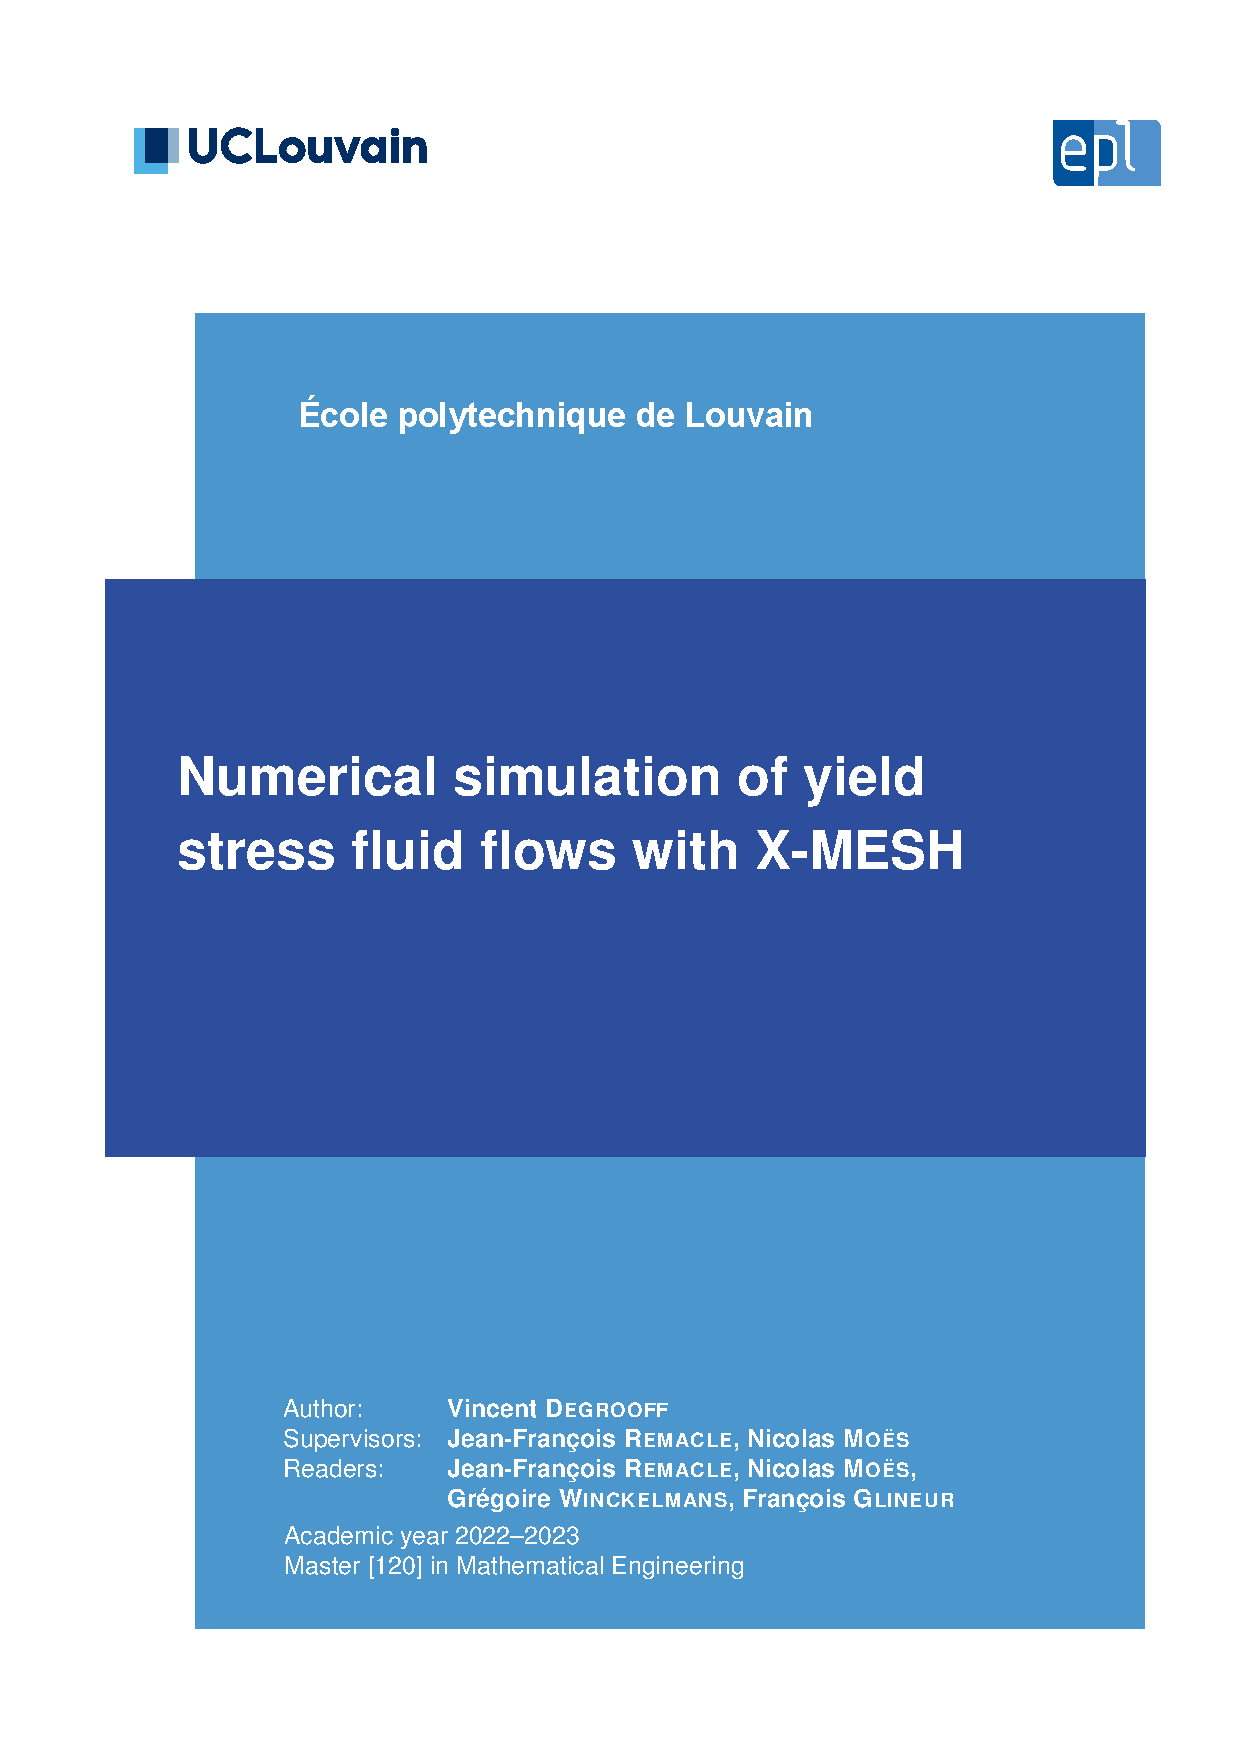
\includepdf[pages=-]{front_page.pdf}
\maketitle

\setcounter{tocdepth}{1}
\tableofcontents

% FOR introduction
%The flow characteristics of such materials are difficult to predict as they involve [...] solid and liquid regions that are generally impossible to locate a priori. CITE Coussot if used so  -->  use X-MESH
% Déboires
%Let us finally get to the crux of this study: the simulation of two-dimensional flows.


% Index i: element
% Index j: node
% Index e: edge
% Index g: Gauss point


\clearpage
\addcontentsline{toc}{chapter}{Introduction}
\chapter*{Introduction}
In the field of fluid mechanics, all fluids are usually divided into two basic categories: Newtonian fluids and non-Newtonian fluids. A fluid is Newtonian when its strain rate, i.e. the change of deformation in the material, is a linear response to viscous stress. By contrast, a fluid is non-Newtonian when its strain rate is not a linear response to viscous stress. Among non-Newtonian fluids, it is possible to distinguish several sub-categories depending on how fluids react to viscous stress.

In this study, we focus on one of these sub-categories: yield stress fluids. These fluids behave like solids when subjected to low stresses, and like liquids otherwise. They therefore present an interface between liquid and solid regions. They encompass some very common substances like blood, hair gel, mayonnaise and cement.

Although these substances are very common and of great importance to the industry, to our knowledge there is no model that precisely locates the solid-liquid interface. The challenge is that it cannot be localized a priori, as its position depends on the stresses, and thus the flow, initially unknown. And yet, a correct localization of this interface provides a substantially better resolution of the physics of the flow.

The aim of this thesis is therefore to couple the flow simulation with an adequate interface tracking on the mesh, i.e. the computational domain discretizing a physical continuum. This thesis is part of the X-MESH project, which aims to track various interfaces that can arise in physics by allowing extreme deformation of meshes. These interfaces can be material, i.e. attached to particles of matter, like the interface between two immiscible fluids, or immaterial like a solidification front or a fire wall crossing a forest. We will see later that we fall into the second category, as yield stress fluid particles can freely move from liquid to solid regions.

The structure of this study is the following. In \cref{chap:chapEq}, we derive the conservation equations along with the constitutive model of the yield stress fluid, to arrive at an energy minimization problem. In \cref{chap:chap1D}, we focus on a flow that is simple enough to be studied in a one-dimensional framework, and we develop a beta version of interface tracking. In \cref{chap:chap2D}, we develop a two-dimensional interface tracking algorithm, which enables us to simulate more complex flows and observe some surprising properties of yield stress fluids.

The code developed for this thesis can be found on the following github repository: \url{github.com/vinzphenix/Bingham_fluid}.

%In the fluid mechanics community, the Newtonian model is so widely used that we often forget that it is a constitutive law, and therefore an approximation. Its assumption is simple, yet accurate for many fluids: the strain rate, the velocity of deformation of its flow, is a linear response to the viscous stress. Its popularity relegates all other fluids to the status of non-Newtonians only, although there are a whole host of them. Here, we will be looking at yield stress fluids, a model that covers substances as common as blood, mayonnaise, hair gel or cement. These fluids are distinguished by their ability to behave like solids when subjected to low stresses.

%We could fool you if we said that the research was carried out because of the importance of these fluids in industry. They may be very present, but what interested us here was the technical aspect of simulating such flows. Indeed, they present an interface between liquid and solid regions, which cannot be localized a priori, as the stresses are initially unknown. Numerical methods, which rely almost exclusively on a discretization of a study domain, therefore generally fail to represent this interface correctly. The aim of this thesis is therefore to couple the flow resolution with an adequate interface tracking.

%To achieve this, we first set the scene in \cref{chap:chapEq}, where we derive the conservation equations along with the constitutive model of the yield stress fluid, to arrive at an energy-minimization problem. Then, in \cref{chap:chap1D}, we focus on a flow that is simple enough to be studied in a one-dimensional framework. This allows us to get our bearings, and to develop a beta version of interface tracking. Finally, in \cref{chap:chap2D}, we tackle the interface capture problem in earnest. This is also an opportunity to observe the surprising properties of yield stress fluid flows.

%More personally, it is an opportunity to put to music the skills I have acquired over the last 5 years as an engineer in applied mathematics, such as numerical methods, optimization, fluid mechanics and programming. The code developed for this thesis can be found on the following github repository: \url{github.com/vinzphenix/Bingham\_fluid}.

\chapter{Governing equations}
\label{chap:chapEq}

\section{General notions of continuum mechanics}
Let $\Omega \in \mathbb{R}^3$ denote the domain of interest and $\Gamma=\partial \Omega$ its boundary. Let $\mathbf{u}$ be the fluid velocity, and $\boldsymbol{\sigma}=-p\mathbf{I}+\boldsymbol{\tau}$ be the stress tensor with its deviatoric contribution $\boldsymbol\tau$.

Let us recall the mass and momentum conservation equations, with the pressure $p$ and body forces $\mathbf{f}$, expressed in an Eulerian reference frame:
\begin{align}
    \nabla \cdot \mathbf{u} &= 0\\
    \rho \left(\pdv{\mathbf{u}}{t} + \left(\mathbf{u} \cdot \nabla\right) \mathbf{u}\right) &= -\nabla p + \nabla \cdot \boldsymbol\tau + \mathbf{f} \label{eq:full_momentum}
\end{align}

%In both yielded and unyielded regions, the stress tensor is continuous (\textcolor{red}{seems obvious, in the yielded zones, but what about the solid part ?}). At the interface, the conservation of mass and momentum read as follows, where $[\![ . ]\!]$ refers to the difference of the fields across the interface and $\mathbf{u^*}$ to the interface velocity:
% \begin{align}
%     [\![ \rho (\mathbf{u^* - \mathbf{u}}) \cdot \mathbf{\hat n} ]\!] &= 0 \label{eq:interface_mass}\\
%     [\![ \rho \mathbf{u} (\mathbf{u^* - \mathbf{u}}) \cdot \mathbf{\hat n} + \mathbf{\hat n} \cdot \sigma ]\!] &= 0 \label{eq:interface_momentum}
% \end{align}

Throughout this study, we consider low Reynolds numbers, i.e. flows that are dominated by viscous forces. We thus neglect the inertia terms on the left of equation \eqref{eq:full_momentum}. 
\begin{empheqboxed}
    \begin{align}
        0 &= -\nabla p + \nabla \cdot \boldsymbol \tau(\uu) + \mathbf{f} &&\text{in} \; \Omega \label{eq:momentum} \\[2pt]
        0 &= \nabla \cdot \uu &&\text{in}\; \Omega \label{eq:mass}\\[6pt]
        \uu &= \mathbf{U} &&\text{on}\; \Gamma_{D} \label{eq:Dirichlet}\\[2pt]
        \boldsymbol \sigma \cdot \nn &= \mathbf{g} &&\text{on}\; \Gamma_{N} \label{eq:Neumann}
    \end{align}
\end{empheqboxed}
The resulting \cref{eq:momentum,eq:mass,eq:Dirichlet,eq:Neumann} are the well known Stokes equations, with the unknown velocity and pressure fields $\uu$ and $p$. $\Gamma_D$ and $\Gamma_N$ are the partitions of the boundary $\partial \Omega$ where Dirichlet and Neumann conditions are applied. $\mathbf{U}$ and $\mathbf{g}$ refer to the velocity and force imposed on the respective partition. $\nn$ is the unitary vector normal to the boundary $\partial \Omega$.
%$\mathbf{U}$ is the velocity imposed on the boundary $\Gamma_{D}$, and $\mathbf{g}$ is the force imposed on the boundary $\Gamma_{N}$. refer to the partitions of $\partial \Omega$ where Dirichlet and Neumann boundary conditions are applied. $\mathbf{U}$ and $\mathbf{g}$ are given beforehand. 

One could also decide to impose only the normal velocity along with the tangential stress, or the tangential velocity along with the normal stress, as will be explained in more detail in \cref{sec:boundary_conditions}.

Before looking for a closure equation for the shear stress tensor, let us first recall the velocity gradient decomposition,
\begin{empheqboxed}
    \begin{align}
        \nabla \mathbf{u} &= \mathbf{D} + \mathbf{W}\\[4pt]
        \mathbf{D} &= \frac{1}{2} \left(\nabla \mathbf{u} + \nabla^T \mathbf{u}\right) = \frac{1}{2} \gam\\[4pt]
        \mathbf{W} &= \frac{1}{2} \left(\nabla \mathbf{u} - \nabla^T \mathbf{u}\right)
    \end{align}
\end{empheqboxed}

%To be exhaustive:
\begin{itemize}[label=---]
    \item $\mathbf{D}$ is the strain rate tensor, whose diagonal elements indicate the stretching of the fluid along the basis vectors and whose off-diagonal elements indicate the shearing of the fluid from one basis vector to another. $\gam$ is the same tensor, scaled by a factor $2$.
    \item $\mathbf{W}$ is the spin tensor indicating the axis around which the flow is locally rotating, as well as the speed of this rotation. It contains the same information as the vorticity vector $\boldsymbol\omega = \nabla \times \vv$.
\end{itemize} 

\section{Constitutive equations of Bingham fluids}

The Newtonian fluid is one of the simplest model of fluid mechanics, as it assumes that the change of deformation of a fluid, or strain rate, is directly proportional to the shear stress it undergoes. This model is highly accurate in describing the behavior of many liquids and gases, such as air, water, gasoline or alcohol, under normal conditions \cite{fox2020fox}. However, it does not characterize inter alia yield stress fluids, such as blood, toothpaste or ketchup, to name a few \cite{Coussot,Geophysical}.

Those non-Newtonian fluids are much better described as \textit{generalized Newtonian} \cite{Geophysical}. This model extends the Newtonian fluid model with a specific nonlinear constitutive law between the stress $\boldsymbol\tau$ and strain rate $\gam$:
\begin{equation}
    \boldsymbol\tau = \mu(\gam, T, \phi) \: \gam
    \label{eq:power-law}
\end{equation}
where $\mu$, $T$ and $\phi$ respectively refer to the fluid viscosity, the temperature and the particle concentration (e.g. polymer chains in dilute solutions). Since the viscosity, a scalar, depends on the tensor $\gam$, then it must depend only on the combinations of components $\gamma_{ij}$ that are not dependent on the coordinate system \cite{bird1987dynamics}. These combinations are the tensor invariants, described below and connected to its eigenvalues $\lambda_i$, as one can find by diagonalizing the matrix $\gam$.
\begin{equation}
    \begin{alignedat}{2}
        I_1(\gam) &\coloneqq \Tr(\gam) &&= \lambda_1 + \lambda_2 + \lambda_3\\
        I_2(\gam) &\coloneqq \frac{1}{2} \left[\big(\Tr(\gam)\big)^2 - \Tr(\gam \cdot \gam)\right] &&= \lambda_1\lambda_2 + \lambda_2\lambda_3 + \lambda_3\lambda_1\\
        I_3(\gam) &\coloneqq \det(\gam) &&= \lambda_1\lambda_2\lambda_3
    \end{alignedat}
\end{equation}

The first invariant is always zero when we deal with incompressible fluids since $\Tr(\gam) = 2 \nabla \cdot \vv$. The third invariant is always neglected because it is also zero for shearing flows in 3 dimensions -- $\vv = u(y)\mathbf{e}_1$ -- precisely those for which the theory was developed. The constitutive law was then later used to model more complex flows, but the absence of $I_3$ has persisted \cite{bird1987dynamics}.

The simplest example of generalized Newtonian fluids are the power-law fluids \cite{bird1987dynamics,Geophysical}, that assume $\mu(\dot\gamma) = K \dot \gamma^{n-1}$, with the \textit{consistency} $K$ and \textit{index} $n$. This can already describe:
\begin{itemize}[label=---, topsep=0pt]
    \setlength{\itemsep}{0pt}
    \item\textit{Shear thinning} fluids with viscosity inversely proportional to strain rate $(n<1)$. For example, Ketchup or blood flow more easily with higher strain rates.
    \item\textit{Shear thickening} or \textit{Dilatant} fluids with viscosity proportional to strain rate $(n>1)$. A typical example called Oobleck, the mixture of cornstarch and water, appears liquid at rest but becomes solid under high deformation because it has become so viscous.
    %that appears liquid at rest, but that becomes viscous enough to walk on it if struck hard enough.
    \item \textit{Newtonian} fluids when $n=1$.
\end{itemize}

However, this model is not sufficient to describe certain fluids under low shear stress. For example, the toothpaste flows like a liquid out of the tube, but stays in its configuration once on the toothbrush, so we can easily put it in our mouth without dropping any on the floor. At low stress, such a fluid is considered to behave as a solid.

The Herschel-Bulkley Model \cite{bird1987dynamics,Geophysical,Coussot} extends the power-law model with a yield stress $\tau_0$ which enables us to simulate yield stress fluids like the toothpaste. When the shear stress tensor norm $\tau < \tau_0$, the fluid behaves as a non-deformable solid ($\gam=\mathbf{0}$) and is called \textit{unyielded}. In these regions, the fluid undergoes rigid-body motion only: either at rest, or in translation, or in rotation, but in any case without deformation.

Above that threshold, the fluid becomes \textit{yielded} and follows the power-law model. The constitutive law of the Herschel-Bulkley Model is represented graphically in \cref{fig:fluid-classification} along with the power-law model, and has the following expression: 
\begin{equation}
    \begin{aligned}
        \dot \gamma_{ij} &= 0 & \text{if} \quad \tau < \tau_0\\
        \tau_{ij} &= \left(K \dot \gamma^{n-1} + \frac{\tau_0}{\dot \gamma}\right) \gamma_{ij} & \text{if} \quad \tau \geq \tau_0\\
    \end{aligned}
    \label{eq:herschel}
\end{equation}
where $\dot \gamma$ and $\tau$ are the square root of the second invariant tensor of $\gam$ and $\boldsymbol\tau$, also equal to their Frobenius norm since they are traceless:
\begin{equation}
    \dot \gamma \coloneqq \sqrt{|I_2(\gam)|} = \sqrt{\frac{1}{2} \, \gam : \gam} = \sqrt{2 \mathbf{D} : \mathbf{D}} \qquad\text{and}\qquad
    \tau \coloneqq \sqrt{|I_2(\boldsymbol\tau)|} = \sqrt{\frac{1}{2} \, \boldsymbol\tau : \boldsymbol\tau}
    \label{eq:tensornorm}
\end{equation}

\begin{figure}[!b]
    \centering
    \includesvg[width=\textwidth]{../figures/fluid_classification.svg}
    \caption{Non-Newtonian fluid models.}
    \label{fig:fluid-classification}
\end{figure}

Common values of $n$ generally lie between $0.3$ and $0.5$, especially for Carbopol gels (e.g. hair gel) and emulsions (e.g. mustard, mayonnaise) \cite{Coussot}. The Bingham model ($n = 1$) is thus very rarely obtained when it is fitted over more than two orders of magnitude of shear rates. The yield stress value $\tau_0$ generally lies in the range [1, 100 Pa] \cite{Coussot}. To give an idea of how common substances fit in this model, several sets of parameters are provided in \cref{tab:parameters}.

Those values are not universal. It is in fact hard to find unanimous parameters values of the Herschel-Bulkley model in the literature, especially for food products because their composition may depend on the brand. For instance, the yield stress of mayonnaise is inversely proportional to its fat content \cite{mayonnaiseFat}. The values may also depend on the test methodology, and on the model for which the experimental data is fitted, which is not always the Herschel-Bulkley model.

\begin{table}[t]
    \centering
    \begin{tabular}[t]{lccc}
        \toprule
        Substance 
        & Yield stress $\tau_0$ $[\mathrm{Pa}]$ 
        & Consistency $K$ $[\mathrm{Pa \, s^n}]$ 
        & Index $n$ $[-]$\\
        \midrule
        Ketchup \cite{ketchup}       & 13 -- 32 & 2--6 & 0.44 -- 0.62 \\[2pt]
        Mayonnaise \cite{mayonnaise1,mayonnaise2} & 75 -- 200 & 10 -- 50 & 0.4 -- 0.65 \\[2pt]
        Molten chocolate at $40^\circ C$ \cite{chocolate} & 8 & 2.4 & 0.88 \\[2pt]
        Hair gel \cite{gel}                     & 60 & 25 & 0.4 \\[2pt]
        \multirow{2}{*}{Toothpaste\cite{toothpaste}}
                                     & $\sim 50$ for children & . & . \\
                                     & $\sim 220$ for adults & . & . \\[2pt]
        Blood \cite{Lee2011}         & $32.5\times 10^{-3}$ & 5.62 & 0.955 \\[2pt]
        \bottomrule
    \end{tabular}
    \caption{Herschel-Bulkley parameters for common substances.}
    \label{tab:parameters}
\end{table}%

The present study will focus on simple yield stress fluids, i.e. those for which the shear stress depends only on the imposed shear rate, and not on time (thixotropic/rheopectic fluids) or shear (elastic behavior of solids) \cite{simpleyield}. Thixotropic fluids have the property that their viscosity \textit{under constant shear} decreases with time. Though less common, rheopectic fluids are the exact opposite because their viscosity increases with 
time. This time dependent viscosity means that those fluids have a memory, more formally called \textit{hysteresis}. Any thixotropic effects will therefore be neglected in this study, since such effects are known to be particularly difficult to model \cite{Coussot,bird1987dynamics}. %This can produce stress-strain rate diagram diagrams with loops, i.e. hysteresis curves, as the.

% INTRODUCTION
Furthermore, only Bingham fluids, i.e. $n=1$, $\tau_0>0$, will be considered hereafter. The equations of this model are indeed simpler to solve than those of the Herschel-Bulkley model in general, but still provide solutions with interfaces that make them interesting to analyze with the X-MESH method. Let us then reformulate model \eqref{eq:herschel} for $n=1$, with $\dot\gamma$ defined in \eqref{eq:tensornorm}:
\begin{empheqboxed}
    \begin{equation}
        \begin{aligned}
            \|\boldsymbol\tau\| &< \tau_0 & \text{if} \quad \gam = \mathbf{0} \\ %\label{eq:tensor_unyielded}
            \boldsymbol{\tau} &= \left(K + \frac{\tau_0}{\dot \gamma}\right) \gam & \text{if} \quad  \gam \neq \mathbf{0} %\label{eq:tensor_yielded}
        \end{aligned}
        \label{eq:constitutive}
    \end{equation}
\end{empheqboxed}

\section{Weak formulation}
\Cref{eq:momentum,eq:mass} are discretized and solved numerically with the finite element method, whose efficiency is well established. It was also the most natural method since it allows interfaces to be represented intrinsically. Before moving on to discretization, however, the system of equations has to be written under its weak form. This is done by multiplying the equations of the strong form by velocity and pressure test functions $\vv \in V$, and $p\in Q$, where:
\begin{align}
    Q &= L^2(\Omega) \coloneqq \left\{q: \Omega \to \mathbb{R} \quad\big\vert\quad \int_\Omega q^2 \dd x < +\infty \right\}\\
    V &= H^1(\Omega)^d \coloneqq \left\{\vv : \Omega \to \mathbb{R}^d \quad\big\vert\quad \int_\Omega \|\vv\|^2 + \|\nabla \vv\|^2 \dd x < +\infty\right\}
\end{align}
%The shear stress tensor $\boldsymbol\tau$ is eventually replaced with its constitutive law \cref{eq:constitutive}.

\begin{equation}
    \begin{aligned}
        0 &= {\color{blue}-\nabla p} + {\color{red} \nabla \cdot \taub(\uu)} + \ff\\
        &= {\color{blue} \int_{\Omega} - \vv \cdot \nabla p \;\dd x} + {\color{red} \int_{\Omega} \vv \cdot (\nabla \cdot \taub) \;\dd x} + \int_{\Omega} \ff \cdot \vv  \;\dd x\\
        &= {\color{blue} \int_{\Omega} p \nabla \cdot \vv - \int_{\Omega} \nabla \cdot (p\vv)} + {\color{red} \int_{\Omega} \nabla \cdot (\taub \cdot \vv) - \int_{\Omega}  \taub (\uu) : \nabla^\top \vv} + \int_{\Omega} \ff \cdot \vv\\
        &= {\color{blue} \int_{\Omega} p \nabla \cdot \vv - \int_{\partial \Omega} p \vv \cdot \nn} + {\color{red} \int_{\partial\Omega} (\taub \cdot \vv) \cdot \nn - \int_{\Omega}  \taub (\uu) : \big(\mathbf{D}(\vv) + \mathbf{\Omega}(\vv)\big)^\top} + \int_{\Omega} \ff \cdot \vv \\
        &= {\color{blue} \int_{\Omega} p \nabla \cdot \vv \;\dd x} - {\color{red} \int_{\Omega}  \taub (\uu) : \mathbf{D}(\vv) \;\dd x} + \int_{\Omega} \ff \cdot \vv \;\dd x + {\color{violet}\int_{\Gamma_N} \mathbf{g} \cdot \vv \; \dd s}\\
        &= {\color{blue} \int_{\Omega} p \nabla \cdot \vv \;\dd x} - {\color{red} \int_{\Omega}  \left( 2K + \frac{\tau_0}{\|\mathbf{D}(\uu)\|} \right) \mathbf{D}(\uu) : \mathbf{D}(\vv) \;\dd x} + \int_{\Omega} \ff \cdot \vv \;\dd x + {\color{violet}\int_{\Gamma_N} \mathbf{g} \cdot \vv \; \dd s}
    \end{aligned}\label{eq:weak_formulation}
\end{equation}
\Cref{eq:weak_formulation} must hold $\forall \; \vv \in H^1(\Omega)^d$ such that $\vv = \mathbf{0} \text{ on } \Gamma_D$. In \cref{eq:weak_formulation}, we initially multiplied \cref{eq:momentum} by a test function $\mathbf{v}$ that is zero on $\Gamma_D$, then and integrated it over $\Omega$. Afterwards, we integrated by parts, used the Divergence theorem, and the property that the double contraction of symmetric and antisymmetric tensors cancels out.

On the other hand, \cref{eq:mass} gets multiplied by a pressure test function $q$.
\begin{equation}
    \begin{aligned}
        \int_{\Omega} q \nabla \cdot \uu &= 0  && \forall q \in L^2(\Omega)
    \end{aligned}
    \label{eq:weak_formulation_p}
\end{equation}


\section{Energy functional}

The velocity field $\uu$ solution of this weak formulation can also be found through an energy functional $\mathcal{J}(\vv)$ \cite{saramito2016complex, Bleyer}. With our hypothesis of low Reynolds number, the viscous forces alone dictate the physics of the problem. We can then assume that viscous dissipation is the only source of internal energy. As in linear elasticity for solids, the infinitesimal work of internal stresses in the deformation is
\begin{equation}
    \begin{aligned}
        W_{\textrm{internal}}(D_{ij}) &= \int_{0}^{D_{ij}} \sigma_{ij} \:\dd D_{ij}'\\
        &= \int -p\delta_{ij} \:\dd D_{ij}' + \int 2K D_{ij}' \:\dd D_{ij}' + {\color{gray} 2} \int \frac{ \: \tau_0 D_{ij}'}{{\color{gray} 2} \sqrt{\frac{1}{2} D_{kl}'D_{kl}'}} \:\dd D_{ij}'\\
        &= -p D_{ii} + K D_{ij} D_{ij} + {\color{gray} 2} \tau_0 \sqrt{\frac{1}{2} D_{ij} D_{ij}}\\
        &= -p \nabla \cdot \uu + 2K \|\mathbf{D}\|^2 + 2\tau_0 \|\mathbf{D}\|\\
        W_{\textrm{internal}}(\uu) &= -p \nabla \cdot \uu + \frac{K}{2} \|\gam(\uu)\|^2 + \tau_0 \|\gam(\uu)\|
    \end{aligned}
    \label{eq:energy_density}
\end{equation}

Note that we managed to eliminate the twofold definition of the constitutive law of Bingham fluids. In fact, the stresses under the yield point $\tau_0$ do not generate any work due to the absence of strain-rate in the non-deformable solid, i.e. $W=\boldsymbol\sigma:\mathbf{D}=\boldsymbol\sigma : \mathbf{0} = 0$.

The total energy of the system $J$ is the work of internal forces diminished by the work of external forces $\int_{\Omega} \ff \cdot \uu + \int_{\Gamma_N} (\boldsymbol \sigma \cdot \nn) \cdot \vv$. We can now reformulate \cref{eq:mass,eq:momentum,eq:Dirichlet,eq:Neumann} as the solution of the optimization problem \eqref{eq:minimize}.
\begin{empheqboxed}
\begin{equation}
    \begin{aligned}
        \uu &= \argmin_{\vv \in \mathcal{V}} \mathcal{J}(\vv)\\[8pt]
        \mathcal{J}(\vv) &= \frac{K}{2}\int_{\Omega} \|\gam(\vv)\|^2 \;\dd x + \tau_0 \int_{\Omega} \|\gam(\vv)\| \;\dd x - \int_{\Omega} \ff\cdot \vv \; \dd x - \int_{\Gamma_N} \mathbf{g} \cdot \vv \;\dd s\\[8pt]
        \mathcal{V} &= \{\vv \;\vert\; \nabla \cdot \vv = 0 \; \text{in} \; \Omega, \: \vv = \mathbf{u}_{D} \;\text{on}\; \Gamma_D \}
    \end{aligned}\label{eq:minimize}
\end{equation}
\end{empheqboxed}

In \cref{eq:energy_density}, we observe that the first term is the incompressibility constraint with its Lagrange multiplier: the pressure $p$, with a minus sign. It is therefore equivalent to set it as a constraint of problem \eqref{eq:minimize}. A scaling analysis shows that the model is intrinsically dependent on just one parameter, the Bingham number $Bn$:
%\begin{equation}
    \begin{gather}
        \vv = U_{\infty}\vv^* \qquad \xx = L \xx^* \qquad \gam = \frac{U}{L} \gam^* \qquad f = \frac{K U_{\infty}}{L^2}f^* \qquad (p,g) = \frac{K U_{\infty}}{L}(p^*,g^*)\\
        Bn = \frac{\tau_0 L}{K U_{\infty}} \qquad \text{yield forces / viscous forces}\\
        \mathcal{J}(\vv^*) = \frac{1}{2}\int_{\Omega} \|\gam^*(\vv^*)\|^2 \;\dd x^* + Bn \, \int_{\Omega} \|\gam^*(\vv^*)\| \;\dd x^* - \int_{\Omega} \ff^*\cdot \vv^* \; \dd x^* - \int_{\Gamma_N} \mathbf{g^*} \cdot \vv^* \;\dd s^*
    \end{gather}
%\end{equation}
% Furthermore, in this study, only homogeneous Neumann boundary conditions will be considered. The boundary integral will therefore be neglected from now on.

We can show that the weak formulation and the energy minimization problem are equivalent. This can be done with a Gâteau derivative of the energy function around its minimum $(\uu, p)$.

\begin{align}
    \mathcal{J}(\uu + \epsilon \vv, p+\epsilon q) &= \int_{\Omega} \frac{K}{2} \|2\mathbf{D}(\uu + \epsilon \vv)\|^2 + \tau_0  \|2\mathbf{D}(\uu + \epsilon \vv)\| \\
    &\qquad - (p + \epsilon q) \nabla \cdot (\uu + \epsilon \vv) - \mathbf{f}\cdot(\uu + \epsilon \vv) \: \dd \xx\\[8pt]
    \|2\mathbf{D}(\uu + \epsilon \vv)\|^2 &= \frac{1}{2} 2\mathbf{D}(\uu + \epsilon \vv) : 2\mathbf{D}(\uu + \epsilon \vv) \nonumber \\
    &= 2 \mathbf{D}(\uu):\mathbf{D}(\uu) + 4\epsilon \mathbf{D}(\uu):\mathbf{D}(\vv) + 2\epsilon^2 \mathbf{D}(\vv):\mathbf{D}(\vv)\\[8pt]
    \left. \dv{\mathcal{J}(\uu + \epsilon \vv, p)}{\epsilon}\right\vert_{\epsilon=0} &= \int_{\Omega} \frac{K}{2}   4\mathbf{D}(\uu):\mathbf{D}(\vv) + \tau_0 \frac{4\mathbf{D}(\uu):\mathbf{D}(\vv)}{2\sqrt{2\mathbf{D}(\uu):\mathbf{D}(\uu)}} - p\nabla\cdot(\vv) - \mathbf{f}\cdot(\vv) \: \dd \xx\nonumber\\
    &= \int_{\Omega} \left(2K + \frac{\tau_0}{\|\mathbf{D}(\uu)\|}\right) \mathbf{D}(\uu):\mathbf{D}(\vv) - p\nabla\cdot \vv - \mathbf{f} \cdot \vv \label{eq:gateau_1} \\[8pt]
    \left. \dv{\mathcal{J}(\uu, p+\epsilon q)}{\epsilon}\right\vert_{\epsilon=0} &= -\int_{\Omega}q \nabla \cdot \uu  \label{eq:gateau_2}
\end{align}

It is clear that $\uu$ is a minimum of $J$ when \eqref{eq:gateau_1} and \eqref{eq:gateau_2} cancel out for every perturbation fields $\vv$ and $q$. Those are precisely the expressions of the weak formulation we derived in \eqref{eq:weak_formulation} and \eqref{eq:weak_formulation_p}.


\chapter{1D solution using conic optimization}
\label{chap:chap1D}

%\section{Introduction}
To start, we will study the well know Poiseuille flow: the fluid is pushed forward by a constant pressure gradient in a channel between two infinitely long plates. This flow is of course a bit boring since it is stationary and fully developed. But it has the merit of being simple to introduce the optimization method in a one-dimensional framework.

We consider $\Omega = [-h/2, h/2]$ that represents a transversal 1D slice of the channel whose width is $h$. We also have that the velocity field reduces to $\mathbf{u} = u(y)\,\ex$, since the flow is $x$ independent and incompressible. The pressure gradient $-\Delta p/\Delta x$ is imposed and considered as a body force $f$. The fluid obviously does not slip at the wall. Furthermore, the symmetry of the problem implies that the shear stress profile satisfies $\tau_{xy}(-y) = -\tau_{xy}(y)$.

%In our 1D case, the interface must have zero velocity $\mathbf{u^*} = \mathbf{0}$, and must be parallel to the flow with $\mathbf{\hat n} = \ey$, both due to the hypothesis of stationary flow. 
%Knowing that, equation \eqref{eq:interface_mass} becomes trivial, and equation \eqref{eq:interface_momentum} enforces continuity of the stress tensor across the interface(s).

\section{Analytic solution}
\label{sec:analytic1D}
We can now solve for $u(y)$. With our hypothesis, the conservation of momentum \eqref{eq:momentum} has boiled down to a scalar equation:
\begin{align}
    0 = f + \pdv{\tau_{xy}}{y} \qquad \implies \qquad \tau_{xy} = -f y \qquad \text{since } \tau_{xy}(0)=0
    \label{eq:tau_xy}
\end{align}

The expression of $\tau_{xy}$ can be obtained from the general expression of the stress tensor in \eqref{eq:constitutive}:
\begin{align}
    \boldsymbol{\tau} &=
    \begin{pmatrix}
        0 & K \partial_y u\\
        K \partial_y u & 0\\
    \end{pmatrix} + \tau_0
    \begin{pmatrix}
        0 & 1\\
        1 & 0\\
    \end{pmatrix} \sign(\partial_y u) \\[6pt] %& \text{if }\quad  \left|\partial_y u\right| > 0
    \implies \tau_{xy} &=
    \begin{cases}
        K \partial_y u - \tau_0  \qquad y > y_0\\[3pt]
        K \partial_y u + \tau_0  \qquad y < -y_0\\
    \end{cases} \label{eq:tau_xy_cases}
\end{align}

The threshold shear-stress is reached at $y=\pm y_0$ when 
\begin{align}
    \tau_{xy}(\pm y_0) = \mp f \, y_0 = \mp \tau_0 \iff y_0 = \frac{\tau_0}{f} \label{eq:threshold}
\end{align}

In view of \eqref{eq:threshold}, the fluid can be totally in the unyielded state when $\frac{\tau_0}{f} \geq \frac{h}{2}$. In that case, its velocity is zero everywhere to satisfy boundary conditions: the fluid is said to be in the \textit{arrested state} \cite{saramito2016complex}.

In the lower zone $[-\frac{h}{2}, -y_0]$, we find the velocity profile $u_3(y)$ by integration equations \eqref{eq:tau_xy} and \eqref{eq:tau_xy_cases}:
\begin{align}
    \int_{-\frac{h}{2}}^y K \pdv{u}{y} + \tau_0 &= \int_{-\frac{h}{2}}^y -f y\\
    u_3(y) &= -\frac{\tau_0}{K} \left(\frac{h}{2}+y\right) + \frac{f}{2K} \, \left(\left(\frac{h}{2}\right)^2 - y^2\right)
\end{align}

The continuity of the velocity field allows us to find the velocity of the plug:
\begin{align}
    u_2 &= u_3(-y_0) = %-\frac{\tau_0}{K} (h+y_0) + \frac{1}{2K} \pdv{p}{x} \, (h^2 - y_0^2)\\
    \frac{f}{8K} \left(h - 2y_0\right)^2
\end{align}

The procedure is very similar for the upper zone $[y_0, h/2]$.

Let us define the non-dimensional coordinate $\eta$, the reference velocity $U_{\infty}$ as the maximum velocity of a classical Poiseuille flow and the Bingham number $Bn$ that relates the yield and viscous stresses.
\begin{align}
    \eta=\frac{2y}{h} \qquad U_{\infty}= \frac{f h^2}{8K} \qquad Bn=\frac{\tau_0 h}{K U_{\infty}}=\frac{8\tau_0}{f h} \qquad \eta_0 = \frac{2y_0}{h} = \frac{Bn}{4}
\end{align}

The velocity profile can then be expressed as follows, in the presence of a yielded region, i.e. when $\eta_0 < 1 \iff Bn < 4$:
\begin{align}
    \frac{u(\eta)}{U_{\infty}} &= -\frac{Bn}{2}(1-\eta) + (1-\eta^2) & \eta_0 < \eta \leq 1\\
    \frac{u(\eta)}{U_{\infty}} &= \left(1 - \frac{Bn}{4} \right)^2 & -\eta_0 \leq \eta \leq \eta_0 \\
    \frac{u(\eta)}{U_{\infty}} &= -\frac{Bn}{2}(1+\eta) + (1-\eta^2) & -1 \leq \eta < -\eta_0
\end{align}

\begin{figure}
    \centering
    \begin{subfigure}[b]{0.41\textwidth}
        \begin{tikzpicture}
  \tikzstyle{ground1}=[fill,pattern=north west lines,draw=none, minimum width=0.75cm,minimum height=0.2cm]
  \tikzstyle{ground2}=[fill,pattern=north east lines,draw=none, minimum width=0.75cm,minimum height=0.2cm]

  \pgfmathsetmacro{\h}{2.25}
  \pgfmathsetmacro{\l}{5.0}
  \pgfmathsetmacro{\b}{1.3}
  \pgfmathsetmacro{\u}{1.5/(1.-\b/4.)^2}
  \pgfmathsetmacro{\xa}{2.75}
  \pgfmathsetmacro{\xb}{-3.5}
  \pgfmathsetmacro{\xc}{0.0}

  \node (wall_up) [ground1, minimum width=2*\l cm, yshift=\h cm, anchor=south] {};
  \draw (wall_up.south east) -- (wall_up.south west);

  \node (wall_down) [ground2, minimum width=2*\l cm, yshift=-\h cm, anchor=north] {};
  \draw (wall_down.north east) -- (wall_down.north west);

  \fill [gray, opacity=0.25] (-\l,-\b*\h/4) rectangle (\l,\b*\h/4);

  \draw (-\l,\b*\h/4) node[black,anchor=east]{} -- (\l,\b*\h/4) ;
  \draw (-\l,-\b*\h/4) node[black,anchor=east]{} -- (\l,-\b*\h/4) ;
  

  % Stress profile (scaled by 0.4)
  \draw ({\xb+0.4*2.0*(\u)/\h}, -\h) -- ({\xb-0.4*2.0*(\u)/\h}, \h);
  \draw[opacity=0.5] (\xb, -\h) -- (\xb, \h);
  \foreach \eta in {-0.75,-0.45,-0.15,0.15,0.45,0.75} {
    \draw[-stealth] (\xb, \h*\eta) -- ({\xb-0.4*2.0*(\u)/\h*\eta}, \h*\eta);
  }
  \node at (\xb, -1.5*\h) {Shear stress};
  \pause

  % Strain profile
  \foreach \eta in {-0.75,-0.45} {
    \draw[-stealth] (\xc, \h*\eta) -- ({\xc+0.4*(\u)/\h*(-\b/2-2*\eta)}, \h*\eta);
  }
  \foreach \eta in {0.45,0.75} {
    \draw[-stealth] (\xc, \h*\eta) -- ({\xc+0.4*(\u)/\h*(\b/2-2*\eta)}, \h*\eta);
  }
  \draw ({\xc+0.4*(\u)/\h*(-\b/2+2)}, -\h) -- (\xc, -\b*\h/4);
  \draw (\xc, +\b*\h/4) -- ({\xc+0.4*(\u)/\h*(\b/2-2)}, +\h);
  \draw[opacity=0.5] (\xc, -\h) -- (\xc, \h);
  % \draw[-stealth] (\xc, \h*0.75) -- ({\xc-0.75*0.75}, \h*0.75);
  % \draw[-stealth] (\xc, \h*0.45) -- ({\xc-0.45}, \h*0.45);
  % %\draw[-stealth] (\xc, \h*0.15) -- ({\xc}, \h*0.15);
  % % \draw[-stealth] (\xc, -\h*0.15) -- ({\xc+0.15}, -\h*0.15);
  % \draw[-stealth] (\xc, -\h*0.45) -- ({\xc+0.45}, -\h*0.45);
  % \draw[-stealth] (\xc, -\h*0.75) -- ({\xc+0.75}, -\h*0.75);
  \node at (\xc, -1.5*\h) {Strain rate};
  \pause

  % Velocity profile
  \draw[opacity=0.5] (\xa+0, -\h) -- (\xa+0, \h);
  \draw ({\xa+\u*(1-\b/4)^2}, -\b*\h/4) -- ({\xa+\u*(1-\b/4)^2}, \b*\h/4);
  \draw  plot[smooth,domain={\b/4}:1] ({\u*((1-\x^2)-\b/2*(1-\x))+\xa}, {\h * \x});
  \draw  plot[smooth,domain={\b/4}:1] ({\u*((1-\x^2)-\b/2*(1-\x))+\xa}, {-\h*\x});
  \draw[-stealth] (\xa, \h*0.75) -- ({\u*((1-(0.75)^2)-\b/2*(1-0.75))+\xa}, \h*0.75);
  \draw[-stealth] (\xa, \h*0.45) -- ({\u*((1-(0.45)^2)-\b/2*(1-0.45))+\xa}, \h*0.45);
  \draw[-stealth] (\xa, \h*0.15) -- ({\xa+\u*(1-\b/4)^2}, \h*0.15);
  \draw[-stealth] (\xa, -\h*0.15) -- ({\xa+\u*(1-\b/4)^2}, -\h*0.15);
  \draw[-stealth] (\xa, -\h*0.45) -- ({\u*((1-(0.45)^2)-\b/2*(1-0.45))+\xa}, -\h*0.45);
  \draw[-stealth] (\xa, -\h*0.75) -- ({\u*((1-(0.75)^2)-\b/2*(1-0.75))+\xa}, -\h*0.75);
  \node at ({\xa+0.5}, -1.5*\h) {Velocity};
  
  \onslide<1->
\end{tikzpicture}

        \vspace{15pt}
    \end{subfigure}
    \begin{subfigure}[b]{0.58\textwidth}
        \includesvg[width=\textwidth]{../figures/poiseuille_bn.svg}
    \end{subfigure}
    \caption{1D problem channel situation, with the velocity and shear-stress profiles.} \label{fig:1D_situation}
\end{figure}


\section{Finite element formulation}

Let us first define the mesh $\Omega=[-h/2, h/2]$ that is made of $n$ elements $\Omega_i=[y_{i-1}, y_i]$, $i=1, \dots, N$, and $N+1$ nodal values $(y_i)$. The velocity profile $u(y)$ is approximated by sum of shape functions $\phi_i$ weighted by their associated nodal value $U_i$. These shape functions have a compact support around their associated node, and satisfy $\phi_j(x_k) = \delta_{jk}$.

\begin{equation}
        u^h(y) = \sum_{j=0}^N U_j \phi_j(y)
\end{equation}

We will consider both linear and quadratic shape functions. They are expressed on a reference element $\hat \Omega = [-1, 1]$ and numbered with local node index $j=1,\dots,n$ in \cref{eq:shape_1D} and \cref{fig:shape_fct_1D}.
\begin{equation}
    \begin{split}
        \phi_1(\eta) &= \frac{1-\eta}{2}\\
        \phi_2(\eta) &= \frac{1+\eta}{2}\\
    \end{split}
    \hspace{40pt}
    \begin{split}
        \phi_1(\eta) &= \frac{1}{2} \, \eta \, (1-\eta)\\
        \phi_2(\eta) &= \frac{1}{2} \, \eta \, (1+\eta)\\
        \phi_2(\eta) &= 1 - \eta^2\\
    \end{split}
    \label{eq:shape_1D}
\end{equation}

\begin{figure}[ht]
    \centering
    \includesvg[width=0.95\textwidth]{../figures/shape_fct_1D.svg}
    \caption{1-dimensional shape functions $\phi$ on the reference element.}
    \label{fig:shape_fct_1D}
\end{figure}


The strain rate tensor with a unidirectional flow $u(y)$ only contains the off-diagonal component,
\begin{equation}
    D_{12}^h(y) = \frac{1}{2} \pdv{u^h}{y} \quad \text{where} \quad \left(\pdv{u^h}{y}\right)_{\Omega_i} = \sum_{j=1}^{n} U_j \dv{\phi_j}{y}
\end{equation}

The minimization function $J$ of \cref{eq:minimize} becomes:
\begin{equation}
\begin{aligned}
    \mathcal{J}(u^h) &= \int_{\Omega} \left[ \frac{K}{2} \left(\pdv{u^h}{y}\right)^2 + \tau_0 \left|\pdv{u^h}{y}\right| - f u^h \right] \dd y\\
    &= \sum_{i=1}^N \int_{\Omega_i} \left[\frac{K}{2}  \left(\pdv{u^h}{y}\right)^2_{\Omega_i} \ + \tau_0 \left|\pdv{u^h}{y}\right|_{\Omega_i} - f u^h\vert_{\Omega_i} \; \right] \dd y\\
    &\approx \sum_{i=1}^N \sum_{g=1}^{ng} \omega_{g} \left[\frac{K}{2}  \left(\pdv{u^h}{y}\right)^2_{y=y_g} \ + \tau_0 \left|\pdv{u^h}{y}\right|_{y=y_g} - f u^h(y_g) \; \right] \frac{\Delta y_i}{2}
\end{aligned}
\end{equation}
where we used Gauss-Legendre quadrature of appropriate order with weights $\omega_g$ and coordinates $y_g$ in the element $\Omega_i$, mapped from coordinates $\eta_g$ in the reference element $[-1,1]$.

In short, one should solve problem \eqref{eq:problem_1D_nonlinear} hereunder
\begin{equation}
    \begin{aligned}
        \textrm{minimize} \qquad & \mathcal{J}(u^h)\\
        \textrm{s.t.} \qquad & u^h(y=-h) = u^h(y=h) = 0
    \end{aligned}\label{eq:problem_1D_nonlinear}
\end{equation}

However, this problem cannot be solved straightforwardly with classical optimization techniques such as gradient descent or Newton's method as it contains a non-differentiable term $|\pdv{u^h}{y}|$. Next section will introduce a suitable method, known as conic optimization.

One could argue that absolute values can be transformed in multiple linear terms in this case. However, this is no longer true as we go to higher dimensions since the tensor norm will become the square root of multiple squared terms. 

\section{Conic optimization in a nutshell}
%CITE NOTES OPTIMIZATION master1
This theory extends linear programming which is restricted to linear cost and linear constraints, by allowing specific nonlinear inequality constraints. For example, $\sqrt{x^2+y^2} \leq z$ is expressed as $(x,y,z) \succeq_{L^3} 0$ or $(x,y,z) \in L^3$, where the Lorentz cone $L^3$ is precisely the set of points $(x,y,z)$ satisfying the nonlinear constraint.

A cone is a subset of a vector space that is closed under linear combinations with positive coefficients. Additional properties can upgrade a cone to a \textit{proper} cone, the only ones we care about in conic optimization. These proper cones $K\subseteq \mathbb{R}^n$ satisfy the following properties:
\begin{enumerate}
    \item $a \succeq_K 0 \implies \lambda a \succeq_K 0 \quad \forall \lambda \in \mathbb{R}^+$ (cone)
    \item $a \succeq_K 0 \text{ and } b \succeq_K 0 \implies a + b \succeq_K 0$ (closed under addition)
    \item $x \succeq_K 0 \text{ and } x \preceq_K 0 \implies x = 0$ (pointed)
    \item $\textrm{int}(K) \neq \emptyset$ (solid)
    \item if $\{x_i\}_{i\to\infty}$ with $x_i \succeq_K 0 \quad \forall i$, then $\lim_{i\to\infty} x_i = \bar x \implies \bar x \succeq_K 0$ (closed)
\end{enumerate}

Cones with such properties will ensure us a global convergence of the Newton's iterations through functions known as \textit{self-concordant barriers}. This is of course very appreciated since Newton's algorithm only converges locally in a general framework.
A function $g:X\to\mathbb{R}$, where $X\subseteq \mathbb{R}^n$ is called self-concordant iff
\begin{itemize}[label=--]
    \item $g \in \mathcal{C}^3$, and
    \item $g$ is convex, and
    \item $\nabla^3 g(x) [h, h, h] \leq 2 \big(\nabla^2 g(x) [h, h]\big)^{3/2} \quad \forall x \in X \quad \forall h \in \mathbb{R}^n$
\end{itemize}
where $\nabla^3 g(x) [h, h, h] = \sum_{i, j, k} \frac{\partial^3 g}{\partial x_i \partial x_j \partial x_k}(x)\: h_i h_j h_k$. With univariate functions $g(x) : \mathbb{R} \to \mathbb{R}$, this last property gets simplified to $|g'''(x)| \leq 2 \big( g''(x) \big)^{3/2}$. Multivariate functions can then be verified to be self-concordant using the univariate test version on $G_{x,h}(t) : \mathbb{R} \to \mathbb{R} : t \mapsto g(x + th) \quad \forall x \in X \quad \forall h \in \mathbb{R}^n$.

Last but not least, self-concordance (s.c.) is preserved through
\begin{itemize}[label=--]
    \item sums: let $f$ and $g$ be s.c. functions, then $h = f+g$ is also a s.c. function.
    \item linear change of variables: let $x \mapsto f(x)$ be a s.c. functions, then $y \mapsto f(A y + b)$ is also a s.c. function.
\end{itemize}

The most common proper cones, with their associated s.c. barrier. are listed in \cref{tab:coefficients}. It may not seem very useful to be limited to such a short list of cones, but a whole zoo of nonlinear constraints can be reformulated to fit in any of these five cones.
\begin{table}
    \centering
    \begin{tabularx}{\textwidth}{@{\extracolsep{\stretch{1}}}*{2}{c}@{}}
        \toprule
        Name & Definition and barrier \\
        \midrule
        Half-space & $\mathbb{R}_+$\\[ 2pt]
         & $g(x) = -\log(x)$ \\[6 pt]
        Lorentz/quadratic cone & $L^{n+1} = \{(x, t) \in \mathbb{R}^n \times \mathbb{R} \quad \vert \quad \|x\|_2 \leq t\}$\\[2 pt]
         & $g(x, t) = -\log(t^2- \|x\|^2)$\\[6 pt]
        Rotated Lorentz cone & $L_R^{n+2} = \{(x, s, t) \in \mathbb{R}^n \times \mathbb{R}_+ \times \mathbb{R}_+ \quad\vert\quad \|x\|_2^2 \leq 2st\}$\\
         & $g(x, s, t) = -\log(2st - \|x\|_2^2)$\\[6 pt]
        Exponential cone & $E = \text{closure} \{(x, y, z) \in \mathbb{R}^3 \quad\vert\quad z \geq y \exp(e/y), y > 0\}$\\[2 pt]
         & $g(x, y, z) = -\log(z - y \exp(e/y)) - \log(y) - \log(z)$\\[6 pt]
        Power cone & $P_{\alpha} = \{(x, y, z) \in \mathbb{R}^3 \quad\vert\quad x^{\alpha} y^{1-\alpha} \geq |z|, x>0, y>0, 0<\alpha<1\}$\\[2 pt]
         & $g(x, y, z) = -\log(x^{2\alpha} y^{2-2\alpha} - z^2) - \log(x) - \log(y)$\\[2 pt]
        \bottomrule
    \end{tabularx}
    \caption{Most frequent proper cones used in conic programming.}
     \label{tab:coefficients}
\end{table}
%In the case of the Lorentz cone $L^3=\{(x,y,z) \vert \sqrt{x^2+y^2} \leq z\}$, the s.c. barrier is $g(x) = -\log(z^2- x^2 - y^2)$. For linear constraints $a^\top x \geq b$, the s.c. barrier is $g(x) = -\log(a^\top x - b)$. Many more cones exists, and there are tables of conic cones with their associated barrier.

Once all the nonlinear constraints have been translated into conic constraints with s.c. barriers $g_i(x)$, the solution is found using an \textit{Interior-point method} that minimizes
\begin{equation}
    f_{\mu} (x) = \frac{c^\top x}{\mu} + \sum_{i} g_i(x)
\end{equation}
where $c$ is the original linear cost and $\mu > 0$ is progressively brought to zero. For each $\mu$, there is an unique solution $x^*_{\mu}$. The set of solutions $x^*_{\mu}$ is called the \textit{central path}. One can eventually retrieve the solution of the original problem since $x^*_{\mu} \to x^*$ as $\mu \to 0$.

Let us take a basic example in 2 dimensions.
\begin{equation*}
\begin{aligned}
    \min_{x,y} \qquad &x\\
    \text{s.t.} \qquad & 2x + y \geq 3 \quad\text{and}\quad 2x - 4y \leq 1 \quad\text{and}\quad x + 5y \leq 10\\
    \implies \qquad & f_{\mu}(x,y) = \frac{x}{\mu} - \log(2x+y-3) - \log(1-2x+4y) - \log(10 - x - 5y)
\end{aligned}
\end{equation*}

\begin{figure}[ht]
    \centering
    \includesvg[width=\textwidth]{../figures/interior_point_example.svg}
    \caption{Solution of the basic example using the interior-point method}
    \label{fig:interior_pt}
\end{figure}

In practice, no one computes the $x^*_{\mu}$ on the \textit{central path} because these points are only used as starting point of the next iteration with a lower $\mu$. Instead, we use an iterative algorithm where we alternate between a Newton step and a decrease of $\mu$ until we reach the required precision. Newton steps keep the current solution close enough to the central path, while the decrease of $\mu$ brings the objective function $f_{\mu}$ to the linear function $c^\top x$. 

For a precision $\epsilon$ s.t. $c^\top x - c^\top x^* < \epsilon$, a solution $x$ is obtained in $\mathcal{O}(\sqrt{\nu} \log \frac{1}{\epsilon})$ iterations with the \textit{short-step algorithm} briefly described here above. $\nu = \sum_{i} \nu_i$, with the barrier parameter $\nu_i$, in a sense related to the \textit{steepness} of the constraint $i$. The initial value x must be close enough to the central path. This can be done with damped Newton steps from any admissible $x \in X$ CITE.

\section{Finite element solution}
\label{sec:fem_1D}
With our recent knowledge in conic programming, we can reformulate problem \eqref{eq:problem_1D_nonlinear} in terms of second order cones only (SOCP).
\begin{empheqboxed}
    \begin{equation}
        \begin{aligned}
            %\min_{s, t, U} \qquad &\sum_{i=1}^n \; \frac{K}{2} s_i \Delta y_i  + \tau_0 t_i \Delta y_i - f \frac{U_{i-1}+U_i}{2} \Delta y_i \\
            \minimize_{U_j, S_{i, g}, T_{i, g}} \qquad &\sum_{i=1}^N \sum_{g=1}^{ng} \omega_{g} \left[\frac{K}{2} \, S_{i, g} + \tau_0 \, T_{i,g} - f u^h(y_g) \; \right] \frac{\Delta y_i}{2}\\
            %\left(\pdv{u^h}{y}\right)^2_{y=y_g}
            %\left|\pdv{u^h}{y}\right|_{y=y_g}
            \textrm{s.t.} \qquad & \left(\pdv{u^h}{y}\right)^2_{y=y_g} \leq S_{i,g} \quad \forall i \:\forall g \qquad \iff \qquad \left[S_{i,g}, \frac{1}{2}, \left(\pdv{u^h}{y}\right)^2_{y=y_g}\right] \in L_R^{3} \quad \forall i \:\forall g\\
            \qquad & \left|\pdv{u^h}{y}\right|_{y=y_g} \leq T_{i,g} \quad \forall i \:\forall g \qquad\;\;\: \iff \qquad \left[ T_{i,g}, \left|\pdv{u^h}{y}\right|_{y=y_g}\right] \in L^{2} \quad \forall i \:\forall g\\
            \qquad & U_0 = U_N = 0
        \end{aligned}
        \label{eq:problem_1D}
    \end{equation}
\end{empheqboxed}

We minimize this problem over the nodal velocities $U$, and the newly added $S$ and $T$ variables. Even if the inequalities may confuse at first glance, they are valid from a modelling standpoint. They are always verified as equalities at the optimum. We can show it by contradiction. Let us assume that $\left(\pdv{u^h}{y}\right)^2 < S_{i,g}$ for a specific index $i,g$ at the optimum. Then the cost can be reduced by decreasing $S_{i,g}$ by $\epsilon > 0$, keeping all other variables unchanged: we are not at the optimum. % fool the solver

At this stage, the finite element solution will be relevant only when the interface is represented on the mesh. Therefore, the arbitrary mesh is manually modified such that two nodes are placed at $y=\pm y_0$. The goal of the next section, is to develop an algorithm that moves the nodes without knowing the interface position beforehand.

The optimization problem was solved with the interior-point solver of the open-source software \texttt{CVXOPT} \cite{cvxopt}. Every simulation presented in this chapter \cref{chap:chap1D} was done with $Bn=2$.

\begin{figure}
    \centering
    \begin{subfigure}[t]{\textwidth}
        \includesvg[width=\textwidth]{../figures/result_1D_P1.svg}
        \vspace*{-12pt}
        \caption{$\mathcal{P}_1$ elements}
        \label{fig:results_1D_P1}
    \end{subfigure}\vspace{6pt}
    \begin{subfigure}[t]{\textwidth}
        \centering
        \includesvg[width=\textwidth]{../figures/result_1D_P2.svg}
        \vspace*{-12pt}
        \caption{$\mathcal{P}_2$ elements}
        \label{fig:results_1D_P2}
    \end{subfigure}\vspace{6pt}
    %\caption{FE solution of the Poiseuille flow with $\mathcal{P}_2$ elements. The unyielded zone is shaded in grey. The error is computed on the whole domain $\Omega$.}
    \caption{FE solution of the Poiseuille flow. The unyielded zone is shaded in grey. The error is shown at the nodes for $u(y)$ and at the reduced integration point for the strain rate and shear.}
\end{figure}


\section{Interface tracking in 1D}

The concept of \textit{front tracking} was initially introduced by James Glimm and co-authors \cite{chern1986front} in the context of hydrodynamics. So I let him define it in his own words \cite{SHE2016383}:
\begin{displayquote}
    Front tracking is the use of surfaces or lower dimensional manifolds as computational degrees of freedom in a numerical algorithm. Its purpose is to improve the resolution of discontinuities or steep gradients in the solution variables or in the laws of physics which describe them.
\end{displayquote}

In our model, the velocity field and even the strain rate field are continuous. In fact, one can infer that on the liquid side of the interface, where $\tau=\tau_0$, the strain rate must also equal to $0$.
\begin{equation}
    \tau_0 = \|\boldsymbol \tau\| \stackrel{\eqref{eq:constitutive}}{=} (K + \tau_0 / \dot \gamma) \|\gam\| = K \dot \gamma + \tau_0 \qquad \implies \qquad \dot \gamma = 0
\end{equation}

The discontinuity is to be found in the derivative of the deformation, e.g. the concavity of the velocity profile in the 1-dimensional case. In fact, $\partial_{yy} u = 0$ in the solid plug as $\partial_y u = 0$ over a whole nonempty interval, while $\partial_{yy} u > 0$ in the liquid region. This is what we observed in \cref{fig:results_1D_P1,fig:results_1D_P2}.

\subsection{Reconstructed strain}

We will therefore make this continuity of the strain rate field our primary objective. Sadly, $\mathcal{P}_1$-elements for the velocity only provide piecewise constant strains, which are of course discontinuous. The idea is thus to reconstruct a continuous strain rate field as a linear approximation of the finite element solution at the Gauss points. This approximation is one-sided at each interface as we should only take the information from the yielded regions.

\begin{algorithm}[!b]
    \caption{Interface tracking algorithm in 1 dimension.}
    \label{alg:tacking_1d}
    optimalMesh $\gets$ false\;
    $\mathcal{M} \gets $ initial mesh with nodes $y_i$\;
    \While{\textsf{not optimalMesh}}{
        Minimize the energy functional $\mathcal{J}$ with $\mathcal{M}$ and retrieve the solutions $U_j, T_{i,g}$\;
        $\mathcal{I} \gets$ set of current interfaces (node shared between yielded and unyielded elements)\;
        \tcp{Stop if $\mathcal{I} = \emptyset$: the mesh should be finer to have unyielded elements}
        %\If{$\mathcal{I} = \emptyset$}{
            %    break \tcp*{Mesh should be finer to have unyielded elements}
            %}
        optimalMesh $\gets$ true\;
        \ForEach {$k \in \mathcal{I}$}{
            $\ell_k \gets$ one-sided linear approximation function of the strain rate close to $y_k$\;
            \If{$\ell_k(y_k) \not\approx 0$} {
                optimalMesh $\gets$ false \tcp*{since $\partial_y u$ is not continuous at the interface}
                $y_k\gets \text{root} (\ell_k(y))$ \tcp*{update $\mathcal{M}$ using the linear approximation}
            }
        }
    }
    \Return $U_j$ 
\end{algorithm}

The choice of Gauss points as abscissae of the linear approximation may seem trivial in this 1-dimensional model case, but the topic was seriously investigated for general geometries. Barlow showed that reduced integration points are superconvergent points, i.e. at which the stress is an order of magnitude more accurate than in any other point within the element \cite{Barlow}. Later on, Zienkiewicz and Zhu developed an error estimator by extrapolating values at the integration points \cite{Zienkiewicz}.

The procedure is described in \cref{alg:tacking_1d} and illustrated in \cref{fig:tracking_1D_P1_steps,fig:tracking_1D_P2_steps}. The strain rate field $\partial_y u$ is shown at each iteration with with its corresponding mesh. The complete overview of the solution is provided for the first and last iterations, for both $\mathcal{P}_1$ and $\mathcal{P}_2$ elements, in \cref{fig:tracking_1D_P1,fig:tracking_1D_P2}.



%Initially, with a random mesh, it is almost certain that the interface (a point) is not represented on the mesh with a node. We can however still compute the solution with the finite element code described in \cref{sec:fem_1D}. The nodes will be moved progressively until the continuity of the strain field is ensured.

%%%%%%%%%%%%%%%%%%%%%%  1D tracking P1  -  start  %%%%%%%%%%%%%%%%%%%%%%
\begin{figure}[hb]
    \centering
    \begin{subfigure}[t]{\textwidth}
        \includesvg[width=\textwidth]{../figures/res_P1_iteration_01.svg}
        %\caption{From first to second iteration.}
    \end{subfigure}
    \begin{subfigure}[t]{\textwidth}
        \includesvg[width=\textwidth]{../figures/res_P1_iteration_02.svg}
        %\caption{From second to third iteration.}
    \end{subfigure}
    \caption{Strain rate field and its reconstruction during the interface tracking algorithm. First to second iteration above, and second to third iteration below. Mesh with 5 $\mathcal{P}_1$-elements.}
    \label{fig:tracking_1D_P1_steps}
\end{figure}

\begin{figure}[ht]
    \centering
    \begin{subfigure}[t]{\textwidth}
        \includesvg[width=\textwidth]{../figures/res_P1_first.svg}
        \caption{Initial mesh.}
        \label{fig:tracking_1D_P1_a}
    \end{subfigure}
    \begin{subfigure}[t]{\textwidth}
        \includesvg[width=\textwidth]{../figures/res_P1_last.svg}
        \caption{Final mesh.}
        \label{fig:tracking_1D_P1_b}
    \end{subfigure}
    \caption{Finite element solution of the Poiseuille flow at the start, and after convergence of the algorithm. $\mathcal{P}_1$ elements.}
    \label{fig:tracking_1D_P1}
\end{figure}
%%%%%%%%%%%%%%%%%%%%%%  1D tracking P1  -  end  %%%%%%%%%%%%%%%%%%%%%%

\FloatBarrier
Although the initial velocity profile was far from correct in \cref{fig:tracking_1D_P1_a}, two iterations were enough to bring the nodes to the interface, and provide an accurate numerical solution with errors around $10^{-6}$ in \cref{fig:tracking_1D_P1_b}.

Surprisingly the convergence is faster for $\mathcal{P}_1$-elements (piecewise constant strain rate) than for $\mathcal{P}_2$-elements (piecewise linear strain rate). This can be easily explained by a flaw in \cref{alg:tacking_1d}: the reconstruction is made over all the Gauss points of elements near the current interface. However, one of these Gauss point can be inside the unyielded region, as can be seen in \cref{fig:tracking_1D_P2_steps}. In that case, the reconstruction is deteriorated because it uses information from the wrong side, leading to a slower convergence.

%%%%%%%%%%%%%%%%%%%%%%  1D tracking P2  -  start  %%%%%%%%%%%%%%%%%%%%%%
\begin{figure}[hb]
    \centering
    \begin{subfigure}[t]{\textwidth}
        \includesvg[width=\textwidth]{../figures/res_P2_iteration_01.svg}
        \label{subfig:tracking_1D_P2_step_1}
        %\caption{From first to second iteration.}
    \end{subfigure}
    \begin{subfigure}[t]{\textwidth}
        \includesvg[width=\textwidth]{../figures/res_P2_iteration_02.svg}
        %\caption{From second to third iteration.}
    \end{subfigure}
    \caption{Strain rate field and its reconstruction during the interface tracking algorithm. First to second iteration above, and second to third iteration below. $\mathcal{P}_1$ elements.}
    \label{fig:tracking_1D_P2_steps}
\end{figure}

\begin{figure}[ht]
    \centering
    \begin{subfigure}[t]{\textwidth}
        \includesvg[width=\textwidth]{../figures/res_P2_first.svg}
        \caption{Initial mesh.}
    \end{subfigure}
    \begin{subfigure}[t]{\textwidth}
        \includesvg[width=\textwidth]{../figures/res_P2_last.svg}
        \caption{Final mesh.}
    \end{subfigure}
    \caption{Finite element solution of the Poiseuille flow at the start, and after convergence of the algorithm. $\mathcal{P}_1$ elements.}
    \label{fig:tracking_1D_P2}
\end{figure}
%%%%%%%%%%%%%%%%%%%%%%  1D tracking P2  -  end  %%%%%%%%%%%%%%%%%%%%%%



\FloatBarrier
\subsection{Energy-based tracking}
An alternative approach was considered for the interface tracking. It consists in minimizing the functional not only over the nodal values, but also over the position of the nodes. Two difficulties then arose. The first one is that the optimization problem becomes non-convex, because of the body force term $fu^h(y_g)$.
\begin{equation}
    \minimize_{U_j, y_i} \sum_{i} \sum_{g} -f \sum_{j=1}^{n} U_{j} \phi_j(y_g) \frac{\Delta y_i}{2}
\end{equation}
where the product $U_j (y_{i}-y_{i-1})$ is obviously not convex in the variables $U_j, y_i, y_{i-1}$ since $U_j$ can be positive or negative. This issue could be overcome by first solving the optimization problem with the velocities as variables, and then fix the velocities while minimizing over the nodal positions. This problem is in fact convex because the three terms of \eqref{eq:problem_1D} are convex in $y_i$:
\begin{align}
    \left(\pdv{u^h}{y}\right)^2 \Delta y_{i} = \left(\sum_j U_j\pdv{\phi}{\eta} \frac{2}{\Delta y_i}\right)^2 \Delta y_{i} &\qquad \text{convex when } \Delta y_i > 0\\
    \left|\pdv{u^h}{y}\right| \Delta y_{i} = \left|\sum_j U_j\pdv{\phi}{\eta} \pdv{\eta}{y}\right| \Delta y_{i} = 2\left|\sum_j U_j\pdv{\phi}{\eta} \right| &\qquad \text{convex because constant in } y_i\\
    -f\sum_j U_j \phi_j \Delta y_i &\qquad \text{convex because linear in } y_i
\end{align}

The second difficulty is even greater: the optimum of this problem (fixing the nodal values or not) is not a mesh with nodes placed at the analytical interface: with $\mathcal{P}_1$ elements, the energy functional can be better minimized by \textit{wrongly} placing the nodes. An example is shown in \cref{fig:sensibility_exact,fig:sensibility_exact} with a mesh of only four nodes.

\begin{figure}[!b]
    \centering
    \includesvg[width=\textwidth]{../figures/sensibility_1D_exact.svg}
    \caption{Nodes at the interface: $\mathcal{J}(u^h) = \mathcal{J}(u^*) + 1.302\times 10^{-3}$.}
    \label{fig:sensibility_exact}
\end{figure}
\begin{figure}[!t]
    \centering
    \includesvg[width=\textwidth]{../figures/sensibility_1D_bad.svg}
    \caption{Optimal nodes: $\mathcal{J}(u^h) = \mathcal{J}(u^*) + 5.787\times 10^{-4}$.}
    \label{fig:sensibility_bad}
\end{figure}

\pagebreak
With $\mathcal{P}_2$, something even stranger happened: a numerical solution $u^h$ claimed to minimize the functional better than the analytical solution $u^*$. This is of course impossible because $u^*$ is the minimum of $\mathcal{J}$ over all fields $u \in H^1(\Omega)$, which includes piecewise quadratic fields (and many more). This nonsense is due to the discrete integration rule, that is unable to exactly integrate the absolute value in the functional: $\mathcal{J} = \dots + \int_{\Omega}\tau_0 \|\gam(\vv^h)\|$. The quadrature succeeds in decreasing the energy with a negative contribution from the integral of a norm, as shown in \cref{fig:sensibility_quad}.

Increasing the number of Gauss points helps, but it comes with the prohibitive cost of adding two variables per element to the optimization problem: $T_{i,g}$ and $S_{i,g}$. A cleverer improvement would be to place an integration point at the boundary of each element, with the Simpson's rule for example.

\begin{figure}[!b]
    \centering
    \includesvg[width=\textwidth]{../figures/sensibility_1D_quadrature.svg}
    \caption{Quadrature: $\mathcal{J}(u^h) = \mathcal{J}^* - 2.36\times 10^{-4}$. Exact integration: $\mathcal{J}(u^h) = \mathcal{J}^* + 2.498\times 10^{-3}$.}
    \label{fig:sensibility_quad}
\end{figure}

% With $\mathcal{P}_2$ elements, this energy-based approach would provide the optimal piecewise quadratic velocity field over all possible meshes. Since, by chance, the analytical solution is quadratic, it would also be the solution of the finite element problem. Hence, the minimization would give the exact velocity field and the correct mesh with nodes at the interface. In that case, it would be impossible to further decrease the cost as the exact solution is optimal over all velocity fields in $H^1(\Omega)$. The approach is however not suitable in general where the exact velocity field is not necessarily part of the finite element space.



\chapter{2D problem}
\label{chap:chap2D}

\section{Finite element formulation}
It is well known that velocity-pressure fields discretized with $\mathcal{P}_1$--$\mathcal{P}_0$ and $\mathcal{P}_1$--$\mathcal{P}_1$ elements do not provide stable discretizations of the Stokes equations, or equivalently of the incompressible linear elasticity equations. A first option is to enrich the velocity space with a bubble function: this is the MINI element \cite{ministable}. A second option is to use Taylor-Hood elements, i.e. $\mathcal{P}_k$--$\mathcal{P}_{k-1}$ for $2 \leq k$. This element was implemented in the code for $k=2$, along with the MINI element. The simulations presented here were done with Taylor-Hood elements unless otherwise specified.

The shape functions $\phi_j$ are represented graphically in \cref{fig:shape_functions_2d}. Again, the finite element approximation velocity field $\vv^h$ is a sum of shape functions attached to each node $j$, weighted by the nodal values $\mathbf{V}_j$:
\begin{align}
    \vv^h(x, y) &= \sum_{j} \mathbf{V}_j \: \phi_j(x, y)
\end{align}

\begin{figure}[t]
    \centering
    \begin{subfigure}[t]{0.495\textwidth}
        \includesvg[width=\textwidth]{../figures/shape_fcts_2d_P1.svg}
        \caption{Lagrange $\mathcal{P}_1$}
    \end{subfigure}
    \begin{subfigure}[t]{0.495\textwidth}
        \includesvg[width=\textwidth]{../figures/shape_fcts_2d_bubble.svg}
        \caption{Bubble enriched Lagrange $\mathcal{P}_1$}
    \end{subfigure}
    \begin{subfigure}[b]{\textwidth}
        \includesvg[width=\textwidth]{../figures/shape_fcts_2d_P2.svg}
        \caption{Lagrange $\mathcal{P}_2$}
    \end{subfigure}
    \caption{Shape functions used for the pressure and velocity fields in 2-dimensions.}
    \label{fig:shape_functions_2d}
\end{figure} 

To express the deformation norm $\|\gam\|$ needed in the functional, we need the velocity gradient:
\begin{align}
    \nabla \vv &= 
    \begin{bmatrix}
        \pdv{u}{x} & \pdv{u}{y}\\
        \pdv{v}{x} & \pdv{v}{y}\\
    \end{bmatrix}\\
    \implies \quad \|\gam(u, v)\|_{\text{Cart}}^2 &= 2 \left(\pdv{u}{x}\right)^2 + \left(\pdv{u}{y} + \pdv{v}{x}\right)^2 + 2\left(\pdv{v}{y}\right)^2
\end{align}

Each of these partial derivatives is also computed as a sum of shape functions derivatives. These spatial derivatives in the physical domain $(x,y)$ are themselves computed from derivatives in the parametric domain $(\xi, \eta)$ through the Jacobian of the transformation.
\begin{align}
    \pdv{u^h_m}{x_n} &= \sum_j U_j \pdv{\phi_j}{x_n} \qquad m=1,2 \quad n=1,2\\
    \left(\nabla_\xx \: \phi\right)_{\text{Cart}} &= \nabla_{\boldsymbol\xi} \phi \; \cdot \dv{\boldsymbol \xi}{\mathbf{x}}\\
    \dv{\boldsymbol \xi}{\mathbf{x}} &= \left(\dv{\mathbf{x}}{\boldsymbol \xi}\right)^{-1} = 
    \begin{bmatrix}
        \pdv{x}{\xi} & \pdv{x}{\eta}\\
        \pdv{y}{\xi} & \pdv{y}{\eta}\\
    \end{bmatrix}^{-1}
\end{align}

The functional of the approximate field $\vv^h$ is recalled below, along with the \textit{weak} incompressibility constraint, where $\psi_l$ denotes the pressure linear shape function, attached to every primary node $l$.
\begin{align}
    \mathcal{J}(u^h, v^h) &= \int_{\Omega} \frac{K}{2} \|\gam(u^h, v^h)\|^2 + \tau_0 \|\gam(u^h, v^h)\| - \mathbf{f} \cdot \vv^h \; \dd x\\
    0 &= \int_{\Omega} \psi_l \; \nabla \cdot \vv^h \qquad \forall \quad \psi_l \label{eq:strong_div}
\end{align}

It is also possible to impose the incompressibility constraint in a \textit{strong} way, i.e. locally at each integration point\cite{Bleyer}. Both options \eqref{eq:weak_div} and \eqref{eq:strong_div} were implemented in the code.
\begin{equation}
    \pdv{u^h}{x} + \pdv{v^h}{y} = 0 \qquad \forall i \; \forall g \label{eq:weak_div}
\end{equation}

\pagebreak
The minimization problem can for Cartesian coordinate systems is given hereunder:% while cylindrical and polar coordinates are detailed in \cref{appendix:curvilinear}.
% \begin{empheqboxed}
%     \begin{equation}
%         \begin{aligned}
%             \minimize_{\mathbf{V}_j, S_{i,g}, T_{i,g}} &\qquad \sum_{i}\sum_{g} \omega_g \left[\frac{K}{2} S_{i,g} + \tau_0 T_{i,g} - \mathbf{f} \cdot \vv^h \vert_{\xx_g} \right] \det \left(\dv{\mathbf{x}}{\boldsymbol \xi}\right)_{i,g}\\
%             &\qquad - \sum_{e}\sum_{g} \tilde \omega_g \,\mathbf{g}\cdot \vv^h\vert_{\xx_g} \frac{\ell_{\text{e}}}{2}\\
%             \textrm{s.t.} &\qquad \left(S_{i,g}, \frac{1}{2}, \sqrt{2}\pdv{u^h}{x}, \sqrt{2}\pdv{v^h}{y}, \pdv{u^h}{y}+\pdv{v^h}{x}\right) \in L_R^5 && \forall i, g\\
%             &\qquad \left(T_{i,g}, \sqrt{2}\pdv{u^h}{x}, \sqrt{2}\pdv{v^h}{y}, \pdv{u^h}{y}+\pdv{v^h}{x}\right) \in L^4 && \forall i, g\\
%             &\qquad 0 = \sum_i \sum_g \omega_g \psi_l \vert_{\xx_g} \left(\pdv{u^h}{x} + \pdv{v^h}{y}\right) && \forall\; l\\
%             &\qquad \mathbf{V}_{j} = \mathbf{u}_{D} && \forall\; \mathbf{V}_{j} \in \Gamma_D
%         \end{aligned}
%     \end{equation}
% \end{empheqboxed}
\begin{empheqboxed}
    \begin{equation}
        \begin{alignedat}{3}
            \minimize_{\mathbf{V}_j, S_{i,g}, T_{i,g}} &\qquad \sum_{i}\sum_{g} \omega_g \left[\frac{K}{2} S_{i,g} + \tau_0 T_{i,g} - \mathbf{f} \cdot \vv^h \vert_{\xx_g} \right] \det \left(\dv{\mathbf{x}}{\boldsymbol \xi}\right)_{i,g}
            - && \: \sum_{e}\sum_{g} \tilde \omega_g \,\mathbf{g}\cdot \vv^h\vert_{\tilde \xx_g} \frac{\ell_{\text{e}}}{2}\\
            \textrm{s.t.} &\qquad \left(S_{i,g}, \frac{1}{2}, \sqrt{2}\pdv{u^h}{x}, \sqrt{2}\pdv{v^h}{y}, \pdv{u^h}{y}+\pdv{v^h}{x}\right) \in L_R^5 && \forall i, g\\
            &\qquad \left(T_{i,g}, \sqrt{2}\pdv{u^h}{x}, \sqrt{2}\pdv{v^h}{y}, \pdv{u^h}{y}+\pdv{v^h}{x}\right) \in L^4 && \forall i, g\\
            &\qquad 0 = \sum_i \sum_g \omega_g \psi_l \vert_{\xx_g} \left(\pdv{u^h}{x} + \pdv{v^h}{y}\right) && \forall\; l\\
            &\qquad \mathbf{V}_{j} = \mathbf{U} && \forall\; \mathbf{V}_{j} \in \Gamma_D
        \end{alignedat}
        \label{eq:functional2D}
    \end{equation}
\end{empheqboxed}
where $\tilde \omega_g$, $\tilde \xx_g$ are the integration weights and positions on the edges, while $\ell_e$ indicates its length.

For this larger scale problem, I switched from \texttt{CVXOPT} \cite{cvxopt} to the \texttt{MOSEK} interior-point solver \cite{mosek} that handles sparse matrices more efficiently, and performs better overall as explained in \cref{tab:solvers}.
\begin{table}[h]
    \centering
    \begin{tabular}[t]{cccc}
        \toprule
         & \texttt{conelp} from \texttt{CVXOPT} \quad & \quad  \texttt{MOSEK} through \texttt{CVXOPT} API \quad & \quad \texttt{MOSEK API}\\
        \midrule
        Nodes & 52 & 350 & 2325\\
        Elements & 60 & 544 & 4202\\
        \midrule
        Optimization variables & 1834 & 15708 & 115643\\
        Linear constraints & 642 & 5566 & 16584\\
        Cones & 360 & 3264 & 25213\\
        \bottomrule
    \end{tabular}
    \caption{Size of the optimization problem \eqref{eq:functional2D} that different solvers are able to solve within $5$ seconds, presolve included for \texttt{MOSEK} (it removes redundant constraints, linear dependencies, \dots).}
    \label{tab:solvers}
\end{table}%

% For example, their in-house solver \texttt{conelp} took $5$ seconds to solve the optimization problem \eqref{eq:functional2D} on a very coarse mesh with only $50$ nodes. Computation time was greatly reduced when I accessed the \texttt{MOSEK} solver from the \texttt{CVXOPT} API: in $5$ seconds, it could solve \eqref{eq:functional2D} over $

Also note that the pressure field can be obtained as the dual variables associated to the incompressibility constraints: either at every primary node in the \textit{weak} case, or at every integration point in the \textit{strong} case.

\section{Boundary conditions}
\label{sec:boundary_conditions}
Boundary conditions should never be overlooked, especially when there are an inflow and outflow in the simulation, as for the Poiseuille flow.

No-slip walls are easily handled, with homogeneous Dirichlet boundary conditions. However, the situation is not as simple at the inflow and outflow. We can list the three most obvious choices:
\begin{enumerate}
    \item Impose the velocity profile at the inflow (Dirichlet)
    \item Impose the pressure at the inflow and at the outflow (Neumann)
    \item Impose the pressure gradient over the domain $\Omega$ (Body force)
\end{enumerate}

However, care must be taken because we are only providing the normal force on the boundary, due to the pressure gradient, but not the tangential force due to the shear stress that is not known yet. If we prescribe only the normal component of the traction $\mathbf{g}=(\nn\cdot\mathbf{\sigma}\cdot\nn)\nn$, we also need to prescribe the tangential component of the velocity $\vv\cdot\tgt$, as can be derived from the weak formulation \cref{eq:weak_formulation} \cite{Bangerth}.

Each description must then be completed in order to obtain a correct physical flow.
\begin{enumerate}[topsep=0pt]
    \setlength{\itemsep}{0pt}
    \item At the inflow, impose the velocity profile with $\vv \cdot \nn = v_n$ and $\vv \cdot \tgt = v_t = 0$. At the outflow, set zero tangential velocity $v_t = 0$, along with a normal force $\mathbf{g} = (-p + \nn\cdot\boldsymbol\tau\cdot\nn)\,\nn = -p_{\text{out}}\nn$. It is not very suitable for Bingham fluids because it requires the knowledge of the velocity profile beforehand.
    \item Impose the normal boundary force at the inflow and outflow, made up of the pressure and normal shear stress: $\mathbf{g} \cdot \nn = -p_{\text{in/out}}$. Also set $v_t=0$ at the two boundaries.
    \item Set the pressure gradient as body force $\mathbf{f} = -\partial_x p$. It still requires to specify the normal shear stress and tangential velocity: $\mathbf{g} = 0 \,\nn$, and $v_t=0$.
\end{enumerate}

If one forgets to cancel the tangential velocity at the outflow, the problem becomes equivalent to impose zero tangential shear stress at the outflow, which is of course not the situation of a Poiseuille flow where $\tau_{12} = K\partial_y u \neq 0$. 

%\pagebreak
I ran a first set of simulations with the correct setup, imposing $v_t=0$, and a second one with the incorrect setup where the condition $v_t=0$ was intentionally forgotten, both without yield stress ($\tau_0=0$). These two situations are compared in \cref{fig:bc_issue_good,fig:bc_issue_bad}. When no condition is applied on the tangential outflow velocity,the finite element solution gives a very high pressure gradient near the outflow corners in order to achieve zero tangential shear force. Also note that the streamlines are curved at the outflow, towards the corners.

One can also wonder if the choice of boundary condition (1-2-3), or the choice of incompressibility condition (weak-strong) influences quality of the solution. In the case of a flow in a channel of 2 meters long and 1 meter wide, the exact energy functional is $-1/12$. The deviation of the numerical functional from the exact functional is given in \cref{tab:setups_compare} for different setups.

% \begin{figure}[t]
%     \centering
%     \begin{subfigure}[t]{0.97\textwidth}
%         \includesvg[width=\textwidth,]{../figures/bc_good.svg}
%         %\caption{From first to second iteration.}
%     \end{subfigure}
%     \begin{subfigure}[t]{0.97\textwidth}
%         \includesvg[width=\textwidth,]{../figures/bc_bad.svg}
%         %\caption{From first to second iteration.}
%     \end{subfigure}
%     \caption{Comparison of the pressure field, streamlines and boundary forces of the correct (top) and incorrect (bottom) flows.}
%     \label{fig:bc_issue}
% \end{figure}
\begin{figure}[H]
    \centering
    \includesvg[width=\textwidth,]{../figures/bc_good.svg}
    \caption{Pressure field, streamlines and boundary forces of the correct flow.}
    \label{fig:bc_issue_good}
\end{figure}
\begin{figure}[H]
    \centering
    \includesvg[width=\textwidth,]{../figures/bc_bad.svg}
    \caption{Pressure field, streamlines and boundary forces of the incorrect flow. Inspired from \cite{stokesBC}.}
    \label{fig:bc_issue_bad}
\end{figure}


\begin{table}[H]
    \centering
    \begin{tabular}[t]{cccc}
        \toprule
         & & Correct setup & Incorrect setup\\
         & & $v_t=0$ & $v_t$ free\\
        Incompressibility & Dirichlet/Neumann & & \\
         & Body force & & \\
        \midrule
        \multirow{2}{*}{Weak} & Dirichlet (1) & $6.095 \times 10^{-10}$ &  $-2.077 \times 10^{-3}$\\
         & Neumann (2) & $2.201 \times 10^{-9}$ &  $-2.130 \times 10^{-3}$\\
         & Body force (3) & $1.858 \times 10^{-11}$ & $-2.130 \times 10^{-3}$\\[4pt]
        \multirow{2}{*}{Strong} & Dirichlet (1) & $7.603 \times 10^{-10}$ &  $-2.037 \times 10^{-3}$\\
         & Neumann (2) & $8.898 \times 10^{-10}$ &  $-2.088 \times 10^{-3}$\\
         & Body Force (3) & $5.483 \times 10^{-10}$ & $-2.088 \times 10^{-3}$\\
        \bottomrule
    \end{tabular}
    \caption{Deviation from the analytical functional: $\mathcal{J}(u^h) - \mathcal{J}(u)$.}
    \label{tab:setups_compare}
\end{table}%


\section{Streamlines computation}
A streamline is a line that is tangential to the instantaneous velocity field. In our case, the streamlines are constant over time as the problem is stationary. They also identical to the pathlines and streaklines.

They can be computed as the path traced out by particles evolving through the flow field, starting from a set of positions $\{\xx^{(i)}\}_{i=1}^n$:
\begin{equation}
    \dv{\xx^{(i)}}{t} = \vv(\xx^{(i)}(t)) \qquad i=1, \dots, n
\end{equation}

There is, however, a more elegant and useful method: computing the level sets of the streamfunction $\boldsymbol{\psi} = \psi(x,y)\,\mathbf{e}_3$. This function is defined for incompressible flow as $\nabla \times \boldsymbol\psi = \vv$, which always ensures the incompressibility constraint. A difference in $\psi$ between two points $A,B\in \Omega$ also indicates the net flux across any curve connecting $A$ and $B$.
\begin{equation}
    \begin{aligned}
        \psi(B) - \psi(A) &= \int_{A}^B \dd \psi = \int_{A}^B \dv{\psi}{x} \dd x + \dv{\psi}{y} \dd y = \int_{A}^B -v \dd x + u \dd y\\
        &= \int_{A}^B (u, v)\cdot (\dd y, -\dd x) = \int_{A}^B \vv \cdot \nn \;\dd\ell
    \end{aligned}
\end{equation}

The level sets of the streamfunction are therefore curves through which the flux is zero, in other words, they are streamlines. Streamlines generated with this method (evenly distributed level sets between $\psi_{\min}$ and $psi_{\max}$), offer a significant advantage over the first method: the flux between any two streamlines is the same everywhere.

Using some vector calculus, one can obtain a relation between the vorticity $\omega$ and the streamfunction $\psi$:
\begin{equation}
    \omega \,\mathbf{e}_3 = \nabla \times \vv = \nabla \times \nabla \times \boldsymbol\psi = \nabla (\nabla \cdot \boldsymbol\psi) - \nabla \cdot \nabla \boldsymbol\psi = - \nabla^2 \psi \,\mathbf{e}_3
\end{equation}

This is the classical Poisson equation, that is easily solved with finite elements, once expressed under its weak formulation. The streamfunction is also discretized with $\mathcal{P}_2$ elements.
\begin{empheqboxed}
    \begin{equation}
        \begin{aligned}
            \psi^h(x,y) &= \sum_{j} \Psi_j \phi_j(x,y) && \text{discretization}\\
            \pdv[2]{\psi}{x} + \pdv[2]{\psi}{y} &= -\omega = -\pdv{v}{x} + \pdv{u}{y} && \text{strong form}\\
            \int_{\Omega} \nabla \psi^h \cdot \nabla \phi_j \;\dd x &= \int_{\Omega} \omega^h \:\phi_j\; \dd x - \int_{\partial \Omega} \phi_j \: \vv^h \cdot \tgt \;\dd \ell \quad \forall \phi_j\qquad && \text{weak form}
        \end{aligned}
    \end{equation}
\end{empheqboxed}
The boundary term $\phi_j \:\vv^h\cdot \tgt$ was deduced from $\phi_j (\nabla \psi^h) \cdot \nn $, so that it can be computed immediately from the velocity field, as $\psi$ is the unknown we are looking for. Since Neumann boundary conditions are used everywhere, the solution $\psi^h$ is defined up to a constant. This can be resolved by imposing $\Psi_j=0$ at for an arbitrary node $j$.

\section{Interface tracking in 2D}
As in the 1D case, we want to the mesh to be topologically correct: the nodes should be placed along the interface between solid and liquid behavior. This will be done in three steps:
\begin{enumerate}
    \item Solve the finite element problem by minimizing the functional $\mathcal{J}$.
    \item Estimate the interface position based on the strain rate field $\gam(\vv^h)$.
    \item Move the nodes of the mesh towards the interface estimation.
\end{enumerate}

The first challenge is that we want to find an interface that is not the root of a scalar field. In such a case, the interface would have been unambiguously located. Unfortunately, in our case, the interface is instead the boundary of the zero level set of $\|\gam(\vv^h)\|$, the latter being a surface of nonzero measure. The idea is therefore to generate a virtual field $\varphi: X \subseteq \Omega \to \mathbb{R}$ whose zero level set would be the interface. It will be done with a predictor–corrector method:
\begin{itemize}
    \item Predict an interface as the boundary of a set of elements having zero deformation at every reduced integration point, i.e. $\{i \;\vert\; T_{i,g} = 0 \;\; \forall\, g\}$.
    \item Construct a virtual field $\varphi$ based on the positive values of strain rate norm $\|\gam(\vv^h)\|$ near the predicted interface. This virtual field will be constructed with local linear approximations of $\|\gam(\vv^h)\|$, in the same idea as in the 1D case. The corrector will be the zero level set of the virtual field: $\{\xx \; \vert\; \varphi(\xx) = 0\}$.
\end{itemize}

In practice, the norm will never be exactly zero, or close to machine epsilon, as we use an interior-point algorithm. Therefore, yielded and unyielded regions will be distinguished with a tolerance parameter $\epsilon$. This $\epsilon$ was tuned to $10^{-4}$, as it provided the best results given that $T_{i,g} \sim 10^{-8}$ inside the unyielded regions, and tends to increases near the interface, even when the mesh is topologically correct.

The procedure described above is detailed in \cref{alg:tacking_2d} and illustrated below for a Poiseuille flow on a mesh with $\sim 2000$ nodes.

\begin{algorithm}[H]
    \caption{Interface tracking algorithm in 2-dimensions.}
    \label{alg:tacking_2d}
    $\mathcal{M} \gets $ initial triangle mesh\;
    \For{i = 1, 2, 3, \dots} {
    %\While{\textsf{not optimalMesh}}{
        \tcp{Step 1}
        Minimize the energy functional $\mathcal{J}$ on the mesh $\mathcal{M}$ and retrieve the solutions $U_j, T_{i,g}$\;
        \tcp{Step 2: Reconstruct a strain rate scalar field with negative values}
        $\mathcal{I} \gets$ set of unyielded elements, i.e. elements $i$ where the strain rate norm $T_{i,g} < \epsilon \; \forall g$\;
        $\mathcal{B} \gets$ set of nodes on the boundary of the connected components of $\mathcal{I}$\;
        \ForEach {$j \in \mathcal{B}$}{
            $\mathcal{N}_j \gets$ set of nodes $n$ close to $j$, i.e. $\text{dist}(n, j) \leq 2$ in the graph\;
            $\mathcal{S}_j \gets$ support of $\mathcal{N}_j$, i.e. elements whose all nodes $\in \mathcal{N}_j$\;
            $\ell_j \gets$ linear approx of $\|\gam(\vv)\|$ on $\mathcal{S}_j$, based on the local $T_{i,g} > \epsilon, \quad \forall i \in \mathcal{S}_j \:\forall g$\;
            $R_n^{(j)} \gets \ell_j(\xx_n) \quad \forall \: n \in \mathcal{N}_j$ \tcp*{evaluate $\ell_j$ on the local support, and store it}
        }
        $\mathcal{N} \gets \cup_{j\in\mathcal{B}} \; \mathcal{N}_j$ \tcp*{compute the union the interface nodes neighbours}
        \ForEach {$n \in \mathcal{N}$}{
            $R_n \gets$ average of the reconstructed values $R_n^{(j)} \; \forall j : n\in \mathcal{N}_j$\;
        }
        $R \gets$ reconstructed strain rate field ($\mathcal{P}_1$), based on nodal values $R_n \; \forall n \in \mathcal{N}$\;
        \tcp{Step 3: move the nodes where the reconstructerd field cancels out}
        $\mathcal{E} \gets$ edges with origin \texttt{org} and destination \texttt{dst} such that $\sign(R_{\text{org}})\neq \sign(R_{\text{dst}})$\;
        $\mathcal{C} \gets \cup_{e\in\mathcal{E}} \big(\text{ adjacent node of }e\text{ closest to the root of }R \text{ along } e\big)$\;
        \ForEach {$c \in \mathcal{C}$}{
            $e\gets$ adjacent edge of $c$, belonging to $\mathcal{E}$, that has the maximal gradient of $R$\;
            $\tilde \xx_{c} \gets$ root of $R$ along $e$\;
        }
        Update the mesh $\mathcal{M}$ with the new positions $\xx_c \gets \tilde \xx_c \: \forall c \in \mathcal{C}$\;
        \tcp{Stop to iterate when every node displacement is smaller than a tolerance}
    }
    \Return $\mathcal{M}$, $U_j$, $T_{i,g}$
\end{algorithm}

\vfill
\begin{figure}[H]
    \centering
    \begin{subfigure}[t]{0.48\textwidth}
        \includesvg[width=\textwidth,]{../figures/rec_2.svg}
        \caption{Zoom on the upper interface of the Poiseuille flow. Gauss point are represented, in color when above the threshold, in grey scale otherwise. The analytical interface is represented as a red line. The predicted unyielded zone is filled in blue grey.}
    \end{subfigure}\hfill
    \begin{subfigure}[t]{0.48\textwidth}
        \includesvg[width=\textwidth,]{../figures/rec_3.svg}
        \caption{Iso-contours of the linear approximation of the strain rate field around one of the nodes of the predicted interface. The reconstruction is only based on the values of the colored Gauss points}
        \label{fig:build_approx}
    \end{subfigure}\vspace{20pt}
    \begin{subfigure}[t]{0.48\textwidth}
        \includesvg[width=\textwidth,]{../figures/rec_4.svg}
        \caption{Evaluation of this linear approximation at every node of the support.}
        \label{fig:eval_approx}
    \end{subfigure}\hfill
    \begin{subfigure}[t]{0.48\textwidth}
        \includesvg[width=\textwidth,]{../figures/rec_7.svg}
        \caption{Level sets of the virtual field. The node displacements are shown as black lines, moving towards the zero level set, not far from the analytical interface, in red.}
        \label{fig:targets}
    \end{subfigure}
    \caption{Description of the 2D interface tracking algorithm. The steps \ref{fig:build_approx} and \ref{fig:eval_approx} are repeated for every node on the predicted interface (the boundary of the blue grey region). After the mesh update \ref{fig:targets}, the finite element problem is solved again, and we repeat the process.}
    \label{fig:rec2d_a}
\end{figure}
\vfill

\begin{figure}[H]
    \centering
    \begin{subfigure}[t]{\textwidth}
        \includesvg[width=\textwidth]{../figures/rect_init.svg}
        \caption{Initial mesh.}
    \end{subfigure}
    \begin{subfigure}[t]{\textwidth}
        \includesvg[width=\textwidth]{../figures/rect_last.svg}
        \caption{Mesh after $7$ iterations: every estimated node displacement was smaller than $10^{-4}$.}
    \end{subfigure}
    \caption{Unyielded elements before and after the interface tracking algorithm. The exact interface is shown in red for comparison. The velocity profile is also shown at the inflow and outflow. This was done on a coarser mesh, with only $\sim 250$ nodes for better visualization.}
\end{figure}

We could also have shown how the velocity and strain rate errors radically decrease once the mesh matches the interface. But it would start a bit repetitive, as the graphs are no different from \cref{fig:results_1D_P2}. Furthermore, we want to study other, slightly more interesting flows.

\section{Narrowing channel flow}
In this situation, we consider a channel whose width narrows from $h_1$ to $h_2$, either suddenly or gradually. A pressure gradient is imposed through Neumann boundary conditions, while the inflow and outflow velocities are forced to be horizontal.

Regardless of the Bingham model, the velocity must increase from the widest to the narrowest section in order to satisfy mass conservation. We can thus expect a slower Poiseuille near the inflow, and a faster Poiseuille near the outflow, with a transition region in between. We can also expect the flow profile to be not only scaled as for Newtonian fluid, but to be qualitatively different as the Bingham number are different in both regions. Using $U_1$ and $U_2$ as mean inflow and outflow velocities, we find that
\begin{equation}
    \begin{aligned}
        U_1 h_1 &= U_2 h_2 &&\text{mass conservation}\\
        Bn_{1} = \frac{\tau_0 h_1}{K U_1} &= \frac{\tau_0 h_2}{K U_2} \frac{h_1^2}{h_2^2} = Bn_{2} \left(\frac{h_1}{h_2}\right)^2
    \end{aligned}
\end{equation}

As $h_1>h_2$, we find $Bn_1>Bn_2$, which is no surprise as the flow upstream is more likely to be unyielded, as the velocity, and thus shear force, are smaller. We can also imagine a situation where $Bn_1>Bn_{\text{crit}}>Bn_2$, where the downstream flow could have been partially liquid, while the upstream flow is beyond the critical Bingham, totally unyielded, and therefore preventing any flow. In fact, $\dot\gamma=0$ enforces uniform motion in translation, or rotation, and the no-slip condition reduces it to $\vv=0$ throughout the solid region.

The results of a simulation are shown in \cref{fig:smoothNeck}, with parameters $K=1$, $\tau_0=0.1$, $h_1=2h_2=1$. We observe that the solid plug we had found in the Poiseuille flow is discontinued in the narrowing region. This is confirmed with the velocity profile in \cref{fig:smoothNeckV}, that is not flat when the channel narrows. 

Furthemore, the width of the solid plugs can be estimated from the analysis we did in \cref{sec:analytic1D}. 
\begin{equation}
    y_0 = \frac{\tau_0}{-\partial_x p} \approx 
    \begin{cases}
        &\frac{0.1}{0.25 / (0.6)} = 0.24\\
        &\frac{0.1}{2 /(3.5-2.25)} = 0.0625\\
    \end{cases}
    \approx
    \begin{cases}
        0.2175 \qquad \text{measured at the inflow}\\
        0.0675  \qquad \text{measured at the outflow}\\
    \end{cases}    
\end{equation}

We also notice on \cref{fig:smoothNeckS} that the left unyielded region has corners. This is in fact a fairly common situation, which will be repeated in subsequent cases.

The type of transition between the smallest and largest width does not significantly modify the flow. With a sudden decrease (\cref{fig:sharpNeck}), two dead zones have nevertheless appeared before the channel narrows. These would typically be recirculation zones with a Newtonian fluid. The deformation is also higher near the corner, though not shown in \cref{fig:sharpNeckS} to keep a meaningful scale. 

\begin{figure}
    \centering
    \begin{subfigure}[t]{\textwidth}
        \includesvg[width=\textwidth]{../figures/neck_smooth_profiles.svg}
        \caption{Velocity profiles.}
        \label{fig:smoothNeckV}
    \end{subfigure}
    \begin{subfigure}[t]{\textwidth}
        %\includesvg[width=\textwidth]{../figures/neck_strain.svg}
        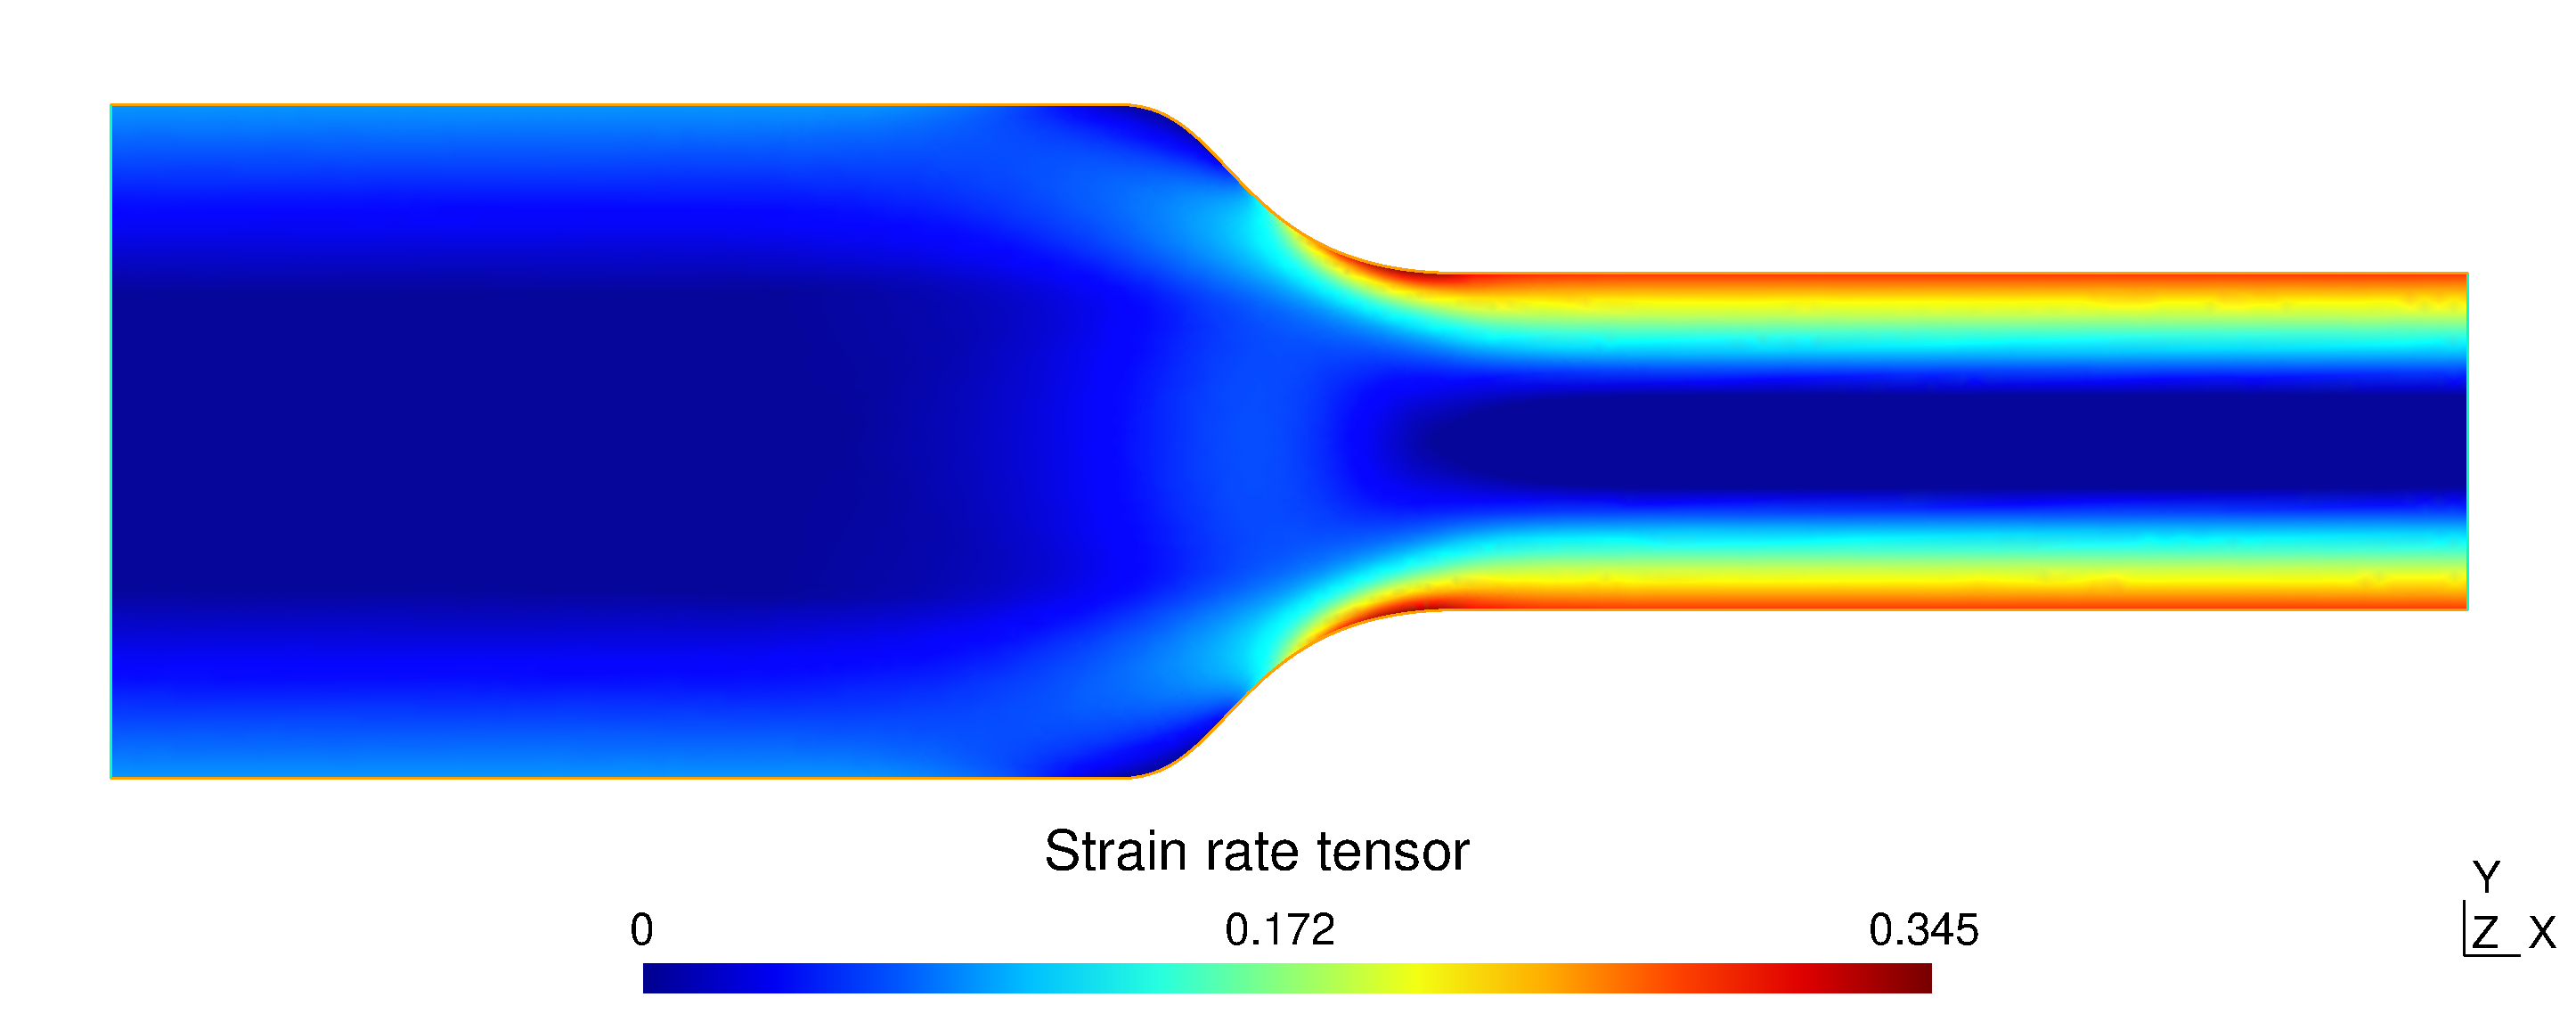
\includegraphics[width=\textwidth]{../figures/neck_smooth_strain.pdf}
        \caption{Strain rate norm.}
        \label{fig:smoothNeckS}
    \end{subfigure}
    \begin{subfigure}[t]{\textwidth}
        \includesvg[width=\textwidth]{../figures/neck_smooth_pressure.svg}
        \caption{Pressure field and streamlines.}
        \label{fig:smoothNeckP}
    \end{subfigure}
    \caption{Visualization of the flow in a smoothly narrowing channel. The unyielded regions are shown in blue grey. Simulation made over a mesh with $12\,000$ elements.}
    \label{fig:smoothNeck}
\end{figure}

\begin{figure}
    \centering
    \begin{subfigure}[t]{\textwidth}
        \includesvg[width=\textwidth]{../figures/neck_sharp_profiles.svg}
        \caption{Velocity profiles.}
        \label{fig:sharpNeckV}
    \end{subfigure}
    \begin{subfigure}[t]{\textwidth}
        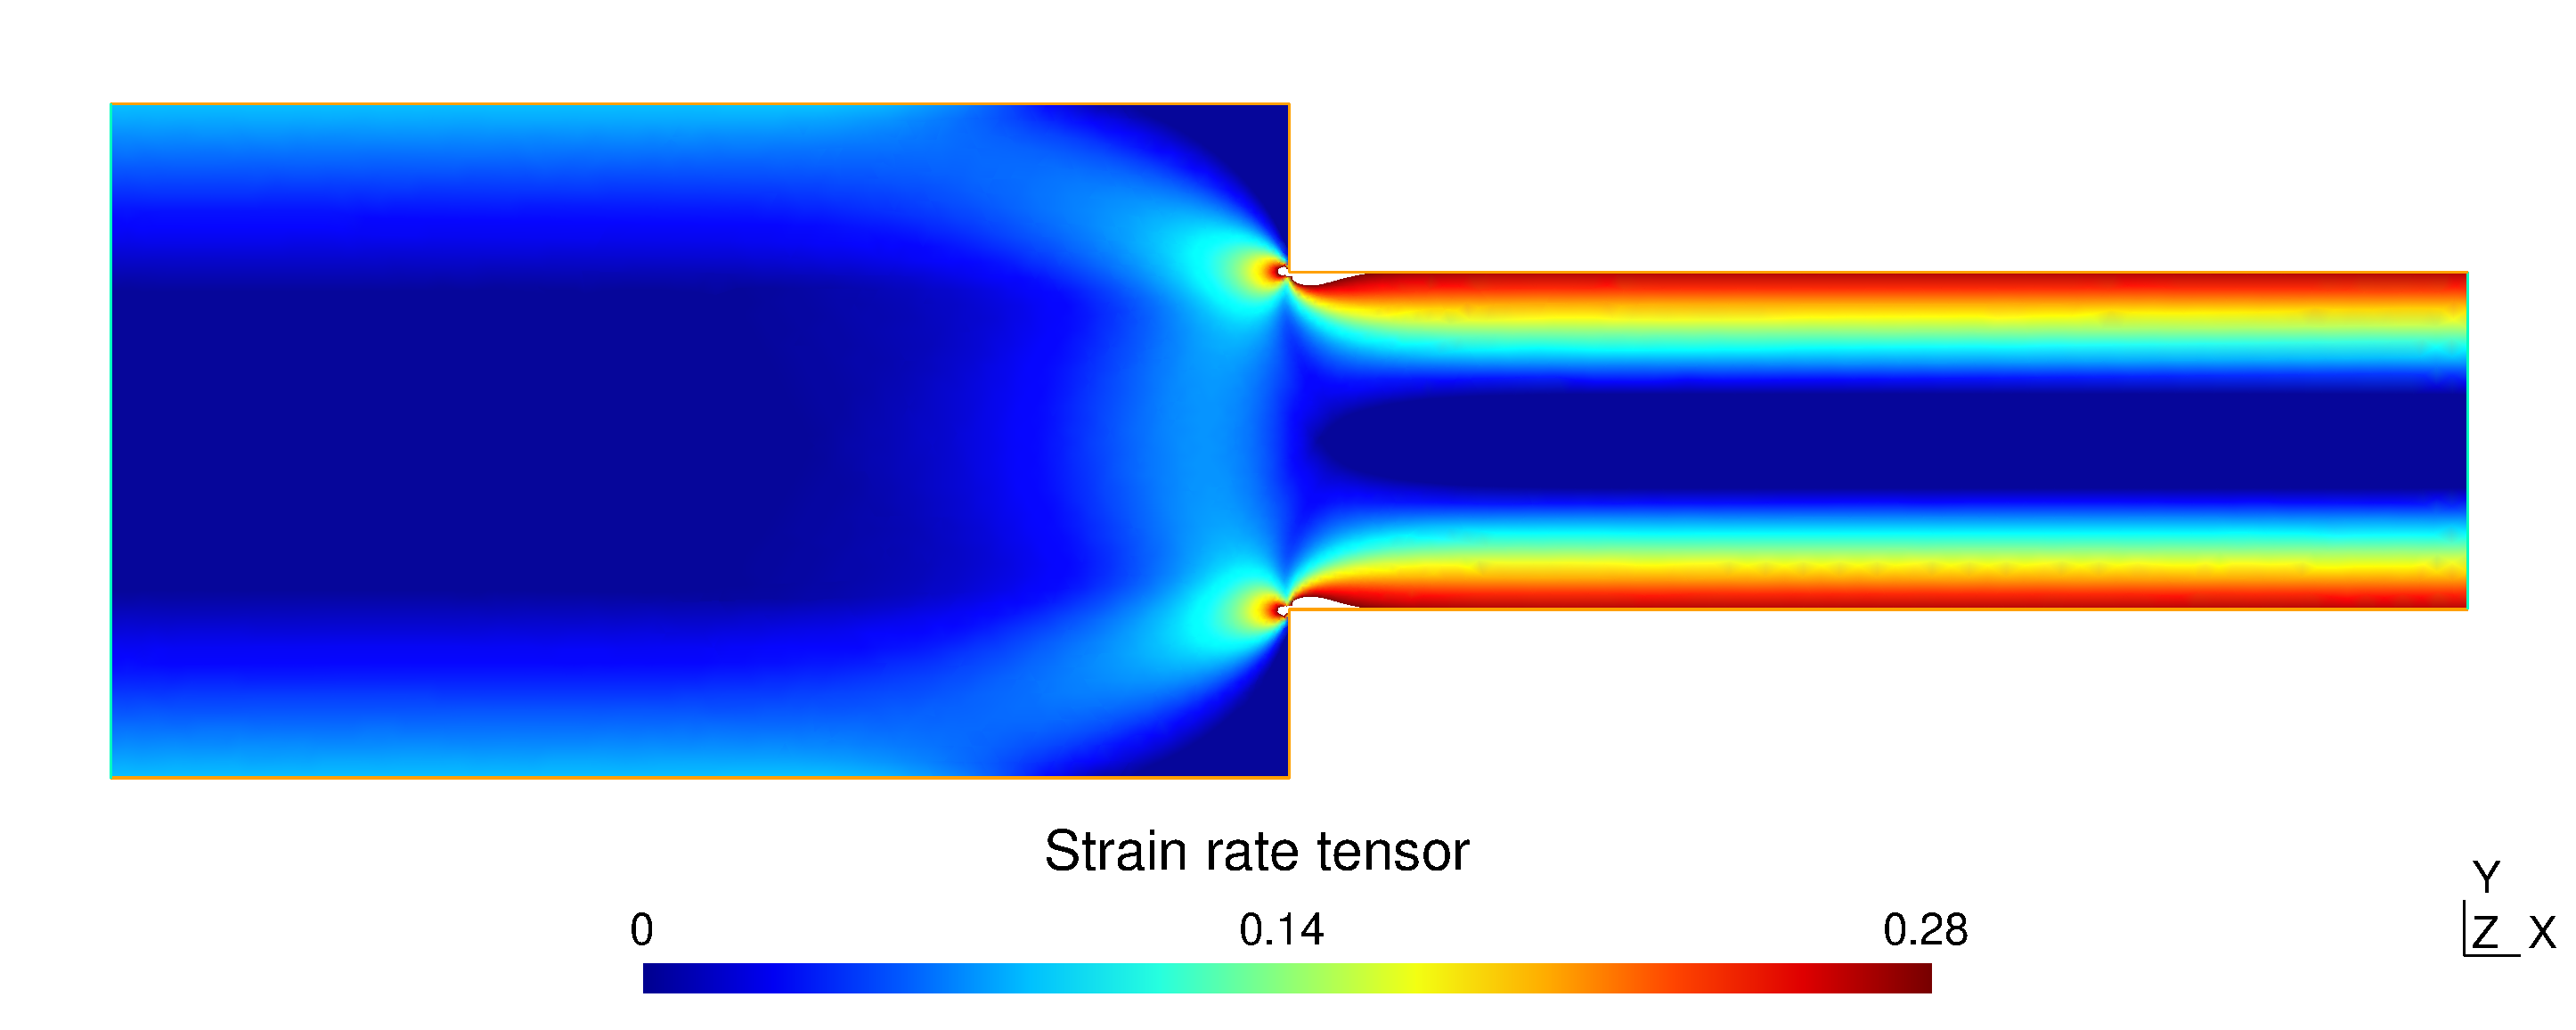
\includegraphics[width=\textwidth]{../figures/neck_sharp_strain.pdf}
        \caption{Strain rate norm.}
        \label{fig:sharpNeckS}
    \end{subfigure}
    \begin{subfigure}[t]{\textwidth}
        \includesvg[width=\textwidth]{../figures/neck_sharp_pressure.svg}
        \caption{Pressure field and streamlines.}
        \label{fig:sharpNeckP}
    \end{subfigure}
    \caption{Visualization of the flow in a forward facing step. Simulation made over a mesh with $14\,000$ elements, denser near the inside corners.}
    \label{fig:sharpNeck}
\end{figure}


\section{Curved channel flow}
In this section, we will finally discover a flow with a rigid rotating zone. To achieve this, we will simulate a flow in a pipe that changes direction along a circular arc of $180^\circ$ after a straight section. Only the upper part of the pipe has been meshed, since the situation is symmetrical.

The features of the flow will be similar to the straight Poiseuille flow: a plug region in the center of the channel, surrounded by two liquid zones near the walls. There is one notable difference, however: the velocity field is not uniform in the solid plug of the turn, it follows a rigid body rotation $\vv(\xx) = \mathbf{W} \times (\xx - \xx_{\text{center}})$.

\begin{figure}[!b]
    \centering
    \begin{subfigure}[t]{\textwidth}
        \includesvg[width=\textwidth]{../figures/pipe_vorticity.svg}
        \caption{Iso-contours of the vorticity. Dashed lines indicate the location of the profiles of \cref{fig:pipeProfiles}.}
        \label{fig:pipeVorticity}
    \end{subfigure}
    \begin{subfigure}[t]{\textwidth}
        \includesvg[width=\textwidth]{../figures/pipe_strain.svg}
        \caption{Average strain rate per element, with a logarithmic scale.}
        \label{fig:pipeStrain}
    \end{subfigure}
    \caption{Visualization of the flow in a in a curved channel. Mesh with $20\,000$ elements, denser near the boundaries, and near the transition from unyielded to yielded. $K=1$, $\tau_0=0.2$, $\text{width}=1$.}
    \label{fig:pipe}
\end{figure}

It can be easily demonstrated that zero deformation implies a constant spin:
\begin{equation}
    \Big[ \gam = \mathbf{0} \quad\text{in}\quad \Omega_s \subseteq \Omega  \;\text{ s.t.}\; \textrm{vol}(\Omega_s) > 0 \Big] \implies \Big[ \nabla \boldsymbol\omega = \mathbf{0} \quad\text{in}\quad \Omega_s\Big]
    \label{eq:constantSpin}
\end{equation}

Hence, in order to modify the vorticity from the staight section plug to the rotating plug, there must be a transition with nonzero deformation, as observed in \cref{fig:pipeStrain}. This deformation is however two orders of magnitude smaller than the one observed near the walls. Furthemore, there seems to be a filament connecting the unyielded regions, with deformations going as low as $10^{-7}$. This does not contradict \cref{eq:constantSpin}, as our curve with vorticity gradient and zero strain rate has zero measure in $\mathbb{R}^2$.

In general, the numerical values of deformation in the solid region typically increase the closer we get to the interface: $\sim 10^{-10}$ deeply inside it and $\sim 10^{-7}$ at the interface. Since the filament exhibits deformations of this order ($\sim 10^{-7}$), and is accompanied by a pressure jump, we can legitimately assume that it is the physical solution, and not an artefact of the interior-point solver.

\begin{figure}[!b]
    \centering
    \begin{subfigure}[t]{\textwidth}
        \includesvg[width=\textwidth]{../figures/pipe_filament_1.svg}
        \caption{Gauss points with deformation $T_{i,g} < 10^{-4} = \epsilon$ (the yield tolerance we set before).}
        \label{fig:pipeFilament1}
    \end{subfigure}\vspace{10pt}
    \begin{subfigure}[t]{\textwidth}
        \includesvg[width=\textwidth]{../figures/pipe_filament_2.svg}
        \caption{Gauss points with deformation $T_{i,g} < 10^{-8}$.}
        \label{fig:pipeFilament2}
    \end{subfigure}
    \caption{Zoom in transition region, on the filament with zero strain rate. Note the streamlines (white curves) going through it, and the discontinuous pressure field (filled iso-contours). The mesh was strongly refined near the filament, with elements $100$ times smaller than the average.}
    \label{fig:pipeFilament}
\end{figure}

\begin{figure}[t]
    \centering
    \includesvg[width=\textwidth]{../figures/pipe_profiles.svg}
    \caption{Slice of different fields in two unyielded regions and in the yielded transition zone.}
    \label{fig:pipeProfiles}
\end{figure}

\Cref{fig:pipeProfiles} illustrates the main features we observed previously:
\begin{itemize}
    \item A velocity profile flat in the straight channel, and inclined towards the outer radius to respect the solid body motion where $\|\vv\| \propto \xx-\xx_{\text{center}}$.
    \item A strain rate profile that is zero over a whole interval at the inflow and outflow. In the transition region however, the strain rate is only zero locally.
    \item The vorticity being constant, either zero for the inflow solid plug or strictly negative for the outflow solid plug.
\end{itemize}

We can derive \cref{eq:pipeCheck} to perform a sanity check of the outflow profile:
\begin{equation}
    \gam=\mathbf{0} \implies 
    \left\{\begin{aligned}
        &\pdv{v}{x} + \pdv{u}{y} = 0\\
        &\pdv{v}{x} - \pdv{u}{y} = \omega_0\\
    \end{aligned}\right\}
    \implies \pdv{v}{x} = -\pdv{u}{y} = \frac{\omega_0}{2}
    \label{eq:pipeCheck}
\end{equation}
\begin{equation}
    2\,\left.\pdv{v}{x}\right\vert_{\text{solid}} \approx 2\,\frac{-0.033 - (-0.024)}{0.6-0.15} = -0.04 \approx \omega\vert_{\text{solid}}
\end{equation}


An analytical solution also exists for the rotating flow of yield stress fluids \cite{circularProfile}. It provides velocity profiles similar to the outflow profile of \cref{fig:pipeProfiles}. The present model could be further validated by precisely quantifying the difference between the numerical and analytical solutions.

\pagebreak
\section{Lid-driven cavity}

The lid-driven cavity is a well known benchmark problem for viscous incompressible fluid flow \cite{FEMfluid}. The geometry and boundary conditions are detailled in \cref{fig:cavitySetup}, along with a modified version of the benchmark inspired from \cite{hoffmann}, that will be studied in a second step.

\begin{figure}[htb]
    \centering
    \begin{tikzpicture}
        \pgfmathsetmacro{\x}{4.}
        \pgfmathsetmacro{\l}{2.5}
        \tikzstyle{groundDw}=[fill,pattern=north east lines,draw=none, minimum width=0.75cm,minimum height=0.2cm]
        \tikzstyle{groundLf}=[fill,pattern=north east lines,draw=none, minimum width=0.2cm,minimum height=0.75cm]
        
        %%%%%%%%%%%%%%%%%%%%%%%%%%%%%%%%%%%%%%%%
        \draw[dashed, line width=1mm, red!60] (-\x-\l,\l) -- (-\x+\l,\l);

        \node at (-\x, 0) (wall_down) [groundDw, minimum width=2*\l cm, yshift=-\l cm,anchor=north] {};
        \draw[line width=1mm, blue!80] (-\x-\l,-\l) -- (-\x+\l,-\l);
        
        \node at (-\x, 0.) (midL) [groundLf, minimum height=2.1*\l cm, xshift=-\l cm, yshift=-0.05*\l cm, anchor=east] {};
        \draw[line width=1mm, blue!80] (-\x-\l,-\l) -- (-\x-\l,+\l);
        
        \node at (-\x, 0.) (midR) [groundLf, minimum height=2.1*\l cm, xshift=+\l cm, yshift=-0.05*\l cm, anchor=west] {};
        \draw[line width=1mm, blue!80] (-\x+\l,-\l) -- (-\x+\l,+\l);
        
        \node at (-\x-\l, \l) (topL) [groundDw, minimum width=0.3*\l cm, xshift=-0.1*\l cm, yshift=-0.05*\l cm, anchor=east] {};
        \node at (-\x+\l, \l) (topR) [groundDw, minimum width=0.3*\l cm, xshift=0.1*\l cm, yshift=-0.05*\l cm, anchor=west] {};
        
        \draw[ultra thick, red!60, ->] (-\x-1,\l*1.1) -- (-\x+1,\l*1.1);
        \draw[ultra thick, ->] (-\x,\l*0.6) arc (90:-180:1);
        
        \node [
            opacity=0.2, shading=axis, rectangle, shading angle=180,
            left color=gray,  right color=gray!20!white,
            minimum width=2*\l cm,  minimum height=2*\l cm
            ] (box) at (-\x, 0.){};
            
        %%%%%%%%%%%%%%%%%%%%%
        \draw[dashed, line width=1mm, red!60] (\x-\l,\l) -- (\x+\l,\l);

        \node at (\x, 0) (wall_down) [groundDw, minimum width=2*\l cm, yshift=-\l cm,anchor=north] {};
        \draw[line width=1mm, blue!80] (\x-\l,-\l) -- (\x+\l,-\l);

        \node at (\x, 0.) (midL) [groundLf, minimum height=(7./6.+0.1)*\l cm, xshift=-\l cm, yshift=1./6.*\l cm, anchor=north east] {};
        \draw[line width=1mm, blue!80] (\x-\l,-\l) -- (\x-\l,+\l/6);

        \node at (\x, 0.) (midR) [groundLf, minimum height=7./6.*\l cm, xshift=+\l cm, yshift=-1./6.*\l cm, anchor=south west] {};
        \draw[line width=1mm, blue!80] (+\x+\l,-\l/6) -- (+\x+\l,+\l);

        \node at (\x-\l, \l) (topL) [groundDw, minimum width=0.4*\l cm, xshift=-0*\l cm, yshift=-0.05*\l cm, anchor=east] {};
        \node at (\x+\l, \l) (topR) [groundDw, minimum width=0.3*\l cm, xshift=0.1*\l cm, yshift=-0.05*\l cm, anchor=west] {};
        
        \draw[ultra thick, red!60, ->] (\x-1,\l*1.1) -- (\x+1,\l*1.1);
        \draw[ultra thick, ->] (\x,\l*0.6) arc (90:-180:1);
        \draw[ultra thick, ->, Green!100] (\x-1.1*\l,0.45*\l) -- (\x-0.8*\l,0.45*\l);
        \draw[ultra thick, ->, Green!100] (\x-1.1*\l,0.65*\l) -- (\x-0.8*\l,0.65*\l);
        \draw[ultra thick, ->, Green!100] (\x+0.8*\l,-0.45*\l) -- (\x+1.1*\l,-0.45*\l);
        \draw[ultra thick, ->, Green!100] (\x+0.8*\l,-0.65*\l) -- (\x+1.1*\l,-0.65*\l);

        \node [
            opacity=0.2, shading=axis, rectangle, shading angle=180,
            left color=gray,  right color=gray!20!white,
            minimum width=2*\l cm,  minimum height=2*\l cm
            ] (box) at (\x, 0.){};
            
        %%%%%%%%%%%%%%%%%%%%%%%%%%%%%%%%%%%%%%%%

        \node (label) at (0., 1.35*\l) [minimum width=3cm, color=red!60]{
            $
            \begin{aligned}
                \vv \cdot \nn &= 0\\
                \vv \cdot \tgt &= -1
            \end{aligned}
            $
        };

        \node (label) at (0., 0.35*\l) [minimum width=3cm, color=Green!100]{
            $
            \begin{aligned}
                \mathbf{g} &= -p\nn \\
                \vv \cdot \tgt &= 0
            \end{aligned}
            $
        };

        \node (label) at (0., -0.55*\l) [minimum width=3cm, color=blue!80]{
            $\vv = \mathbf{0}$
        };
    
    \end{tikzpicture}
    \vspace{6pt}
    \caption{Description of the lid-driven cavity geometry. On the left, the classical setup with no-slip walls in {\color{blue!80} blue} and the upper surface with imposed velocity in {\color{red!60} red}. On the right, the modified setup with inflow/outflow in {\color{Green} green}, where $p=0$. The normal $\nn$ is pointing outwards, and the tangent vector $\tgt$ is oriented anti-clockwise.}
    \label{fig:cavitySetup}
\end{figure}


% \begin{subfigure}[b]{0.45\textwidth}
%     \begin{tikzpicture}
%         \draw (-6,0.75) node[black,anchor=east]{$y=y_0$};
%     \end{tikzpicture}
%     \caption{caption}
%     \label{fig:4b}
% \end{subfigure}


\subsection{Original geometry -- closed cavity}

With a Newtonian fluid, the strain rate cancels at a position slightly below the stagnation point along the center vertical line, and in the two lower corners as shown in \cref{fig:cavity0}. As soon as the Bingham number becomes positive, these three points become surfaces. The two unyielded regions in the corners merge for $Bn\in[1,1.5]$. There, the velocity must be zero to satisfy the no-slip boundary conditions. In the central region however, the fluid follows a solid body rotation, clearly visible in \cref{fig:cavity100} with the circular streamlines.

Higher $Bn$ leads to larger unyielded regions: this has already been observed many times in the literature \cite{Bleyer,Syrakos,Treskatis}. Specifically, the velocity profiles obtained by the present method, by Bleyer et al. \cite{Bleyer} and by Syrakos et al. \cite{Syrakos} are compared in \cref{fig:compareCavity}. 

The mesh used for the simulations contains $12\,000$ elements, denser closer to the upper boundary and the upper corners. The simulation with $Bn=500$ was however done on a finer mesh with $9\,000$ elements, refined inside the the yielded region because the interface tracking did not orginally succeeded. We will come back to the robustness of the algorithm in more detail in \cref{sec:failures}.

Again, there appears to be curves with small deformation emerging from the corners of unyielded region. 

We can also note that the rotating behavior is verified with the velocity profile of \cref{fig:profilesCavity}. Using relation \eqref{eq:pipeCheck} that we derived previously, it comes with no surprise that $\partial_y u$ is constant in the solid rotating region.

\pagebreak

\vfill
\begin{figure}[t]
    \centering
    \begin{subfigure}[t]{0.495\textwidth}
        %\includesvg[width=\textwidth]{../figures/cavity_0.svg}
        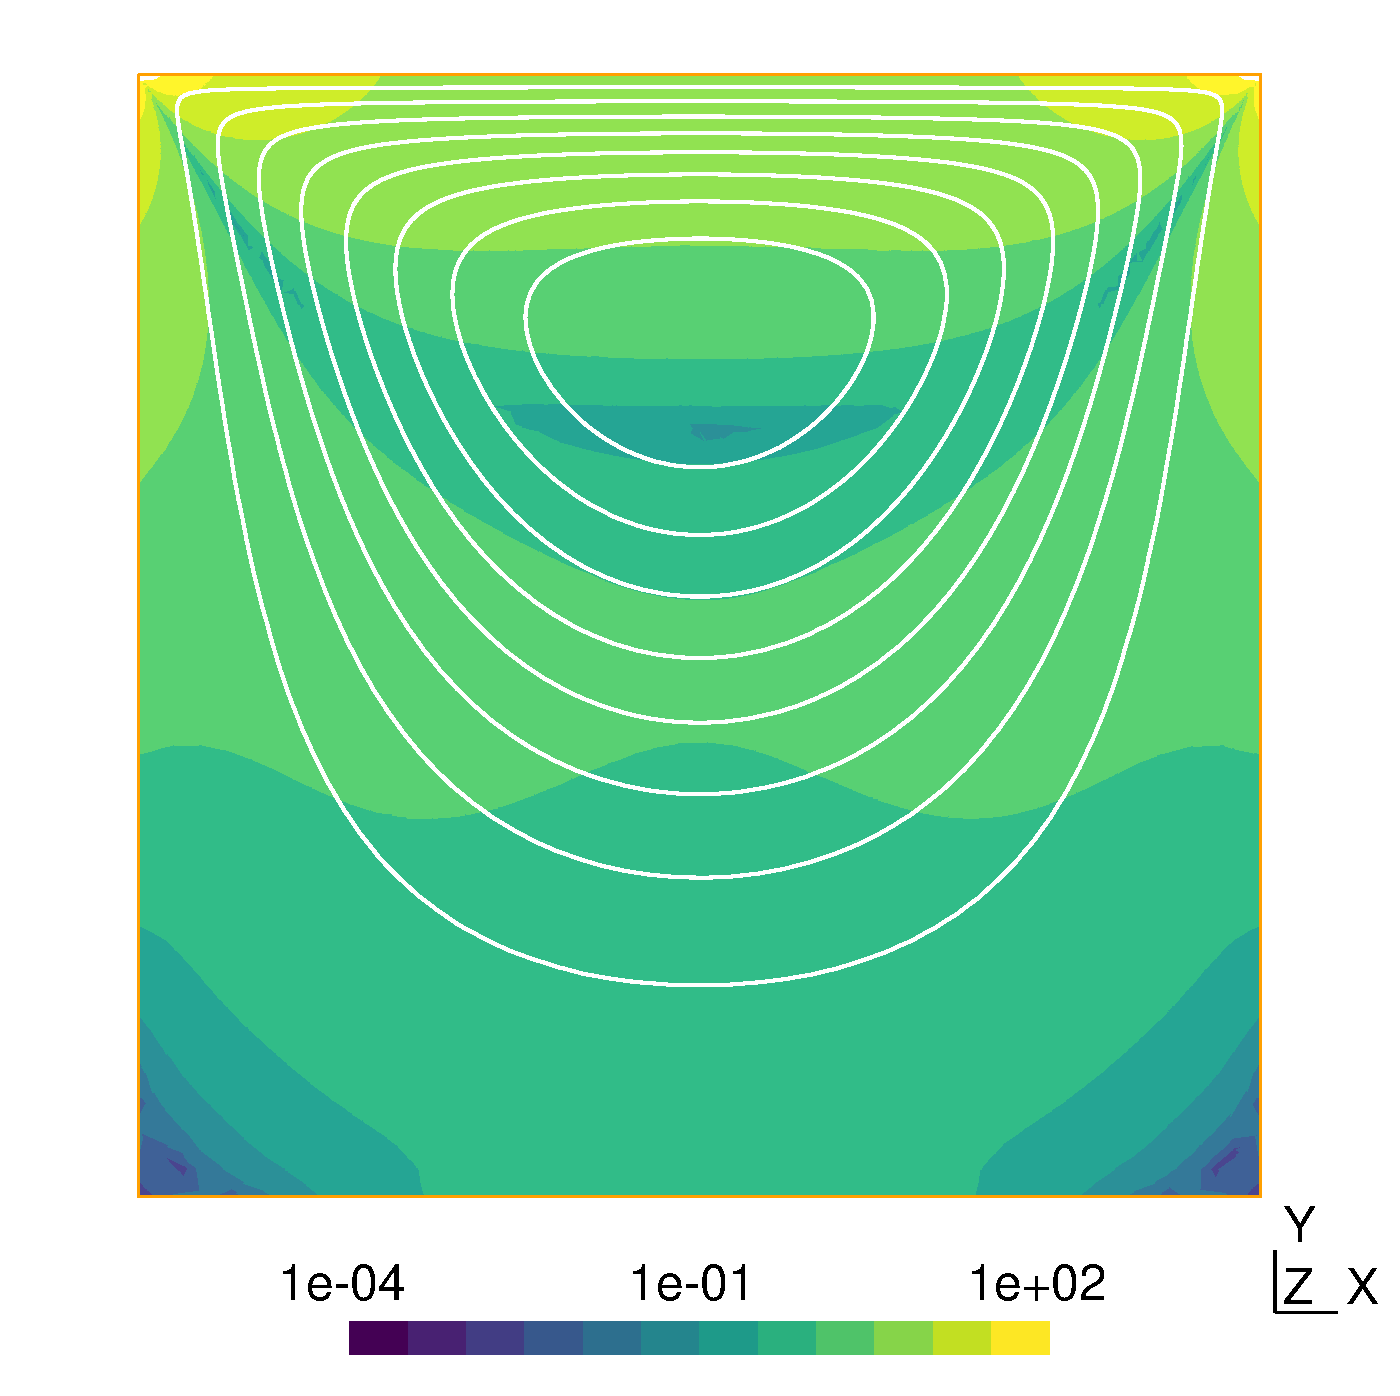
\includegraphics[width=\textwidth]{../figures/cavity_0.pdf}
        \caption{$Bn=0$ (Newtonian fluid)}
        \label{fig:cavity0}
    \end{subfigure}
    \begin{subfigure}[t]{0.495\textwidth}
        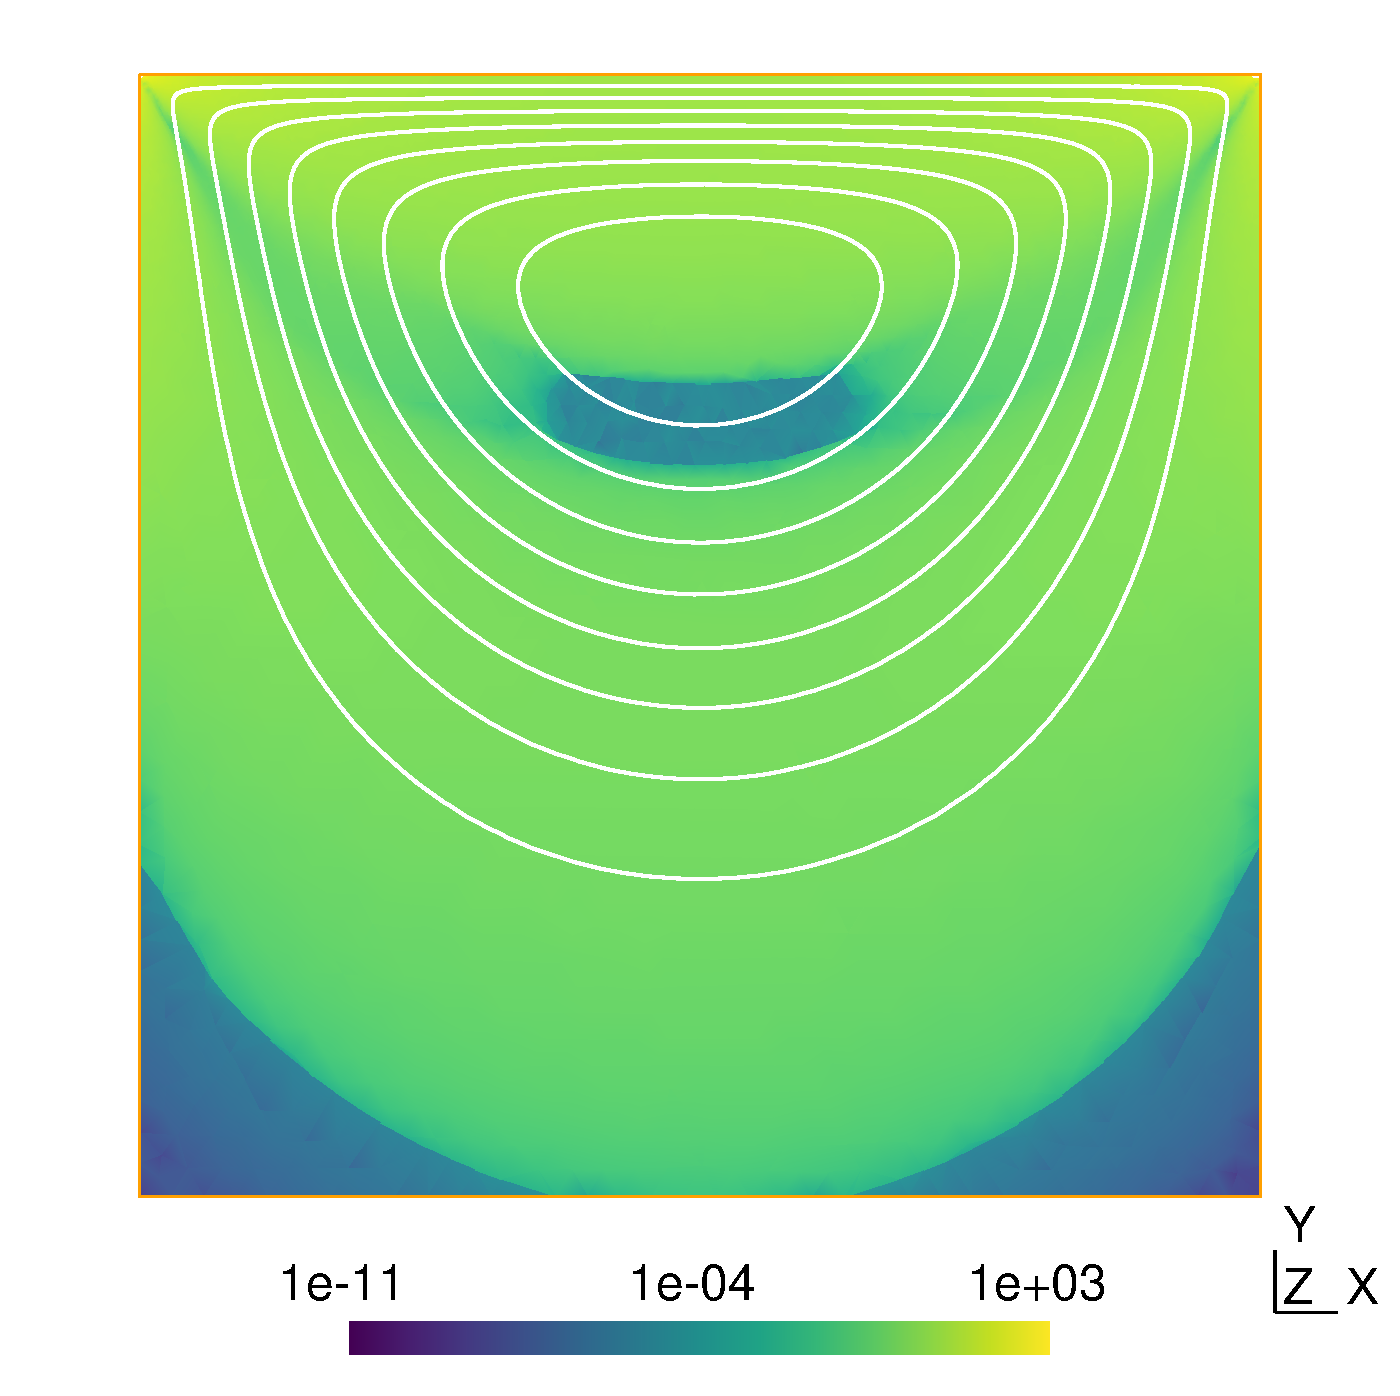
\includegraphics[width=\textwidth]{../figures/cavity_1.pdf}
        \caption{$Bn=1$.}
        \label{fig:cavity1}
    \end{subfigure}
    \begin{subfigure}[t]{0.495\textwidth}
        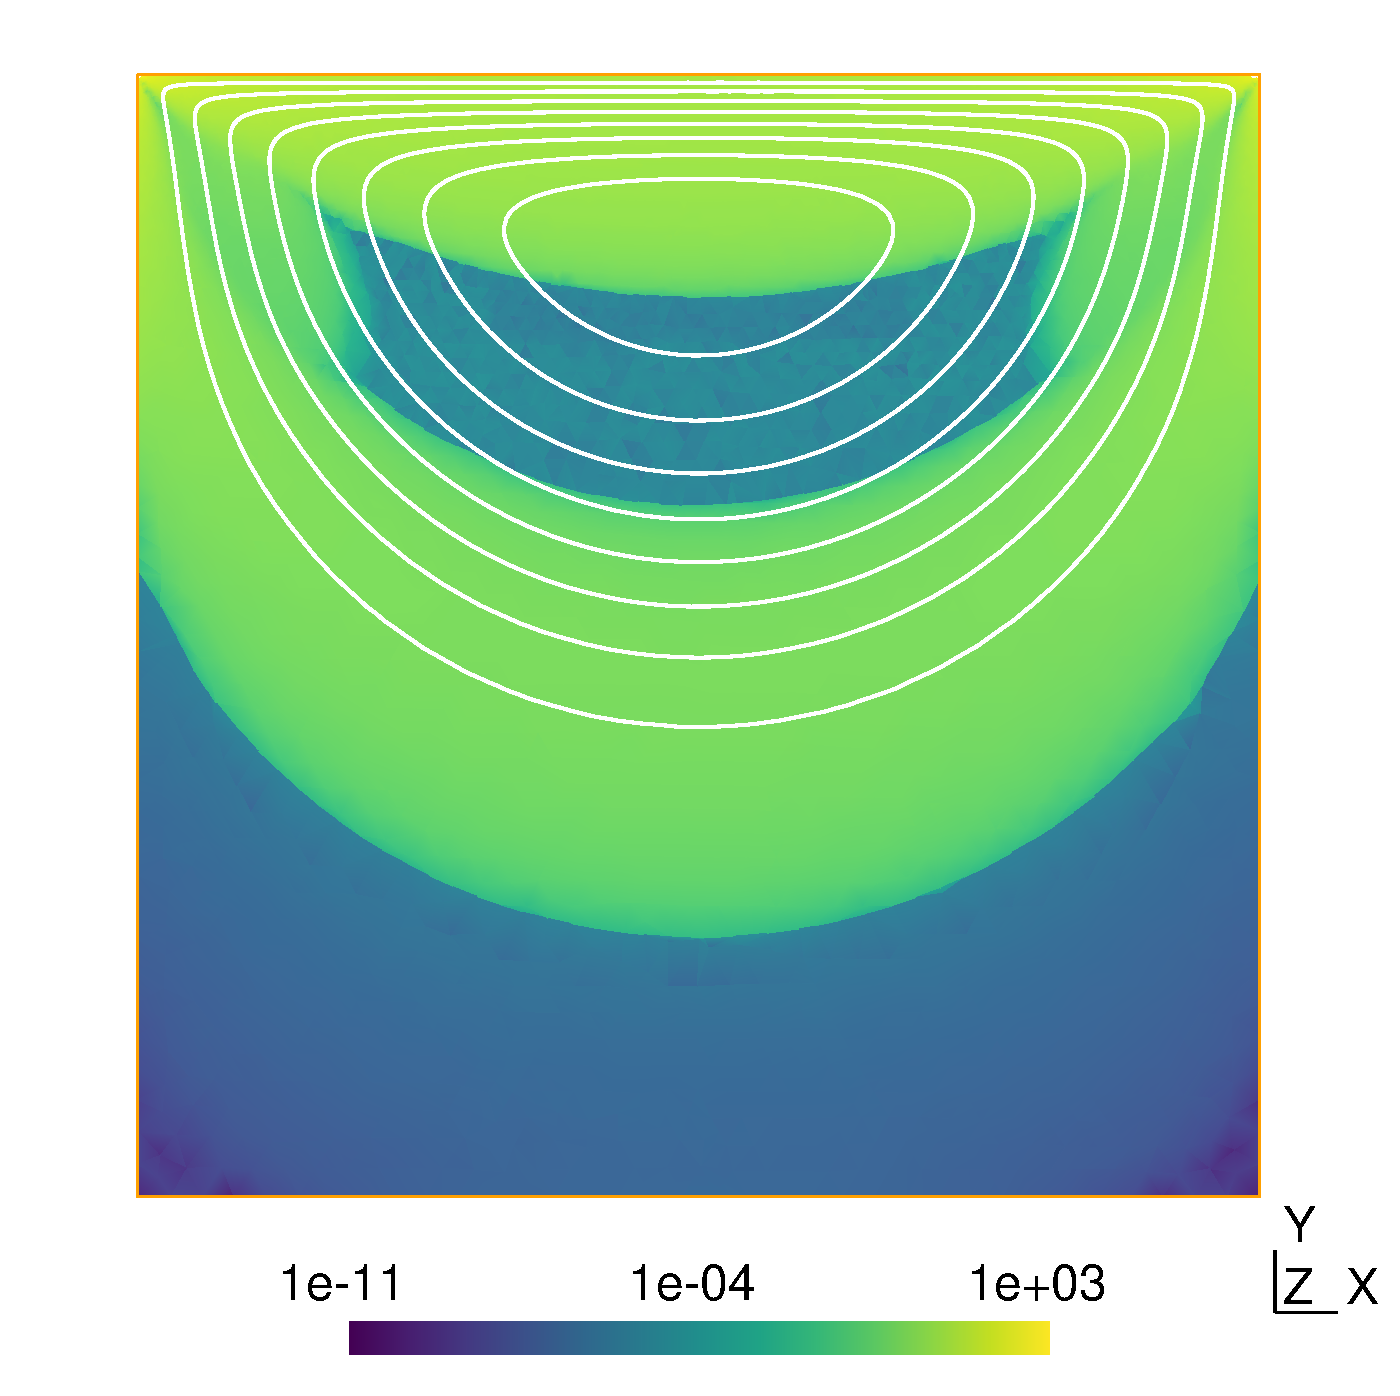
\includegraphics[width=\textwidth]{../figures/cavity_5.pdf}
        \caption{$Bn=5$}
        \label{fig:cavity5}
    \end{subfigure}
    \begin{subfigure}[t]{0.495\textwidth}
        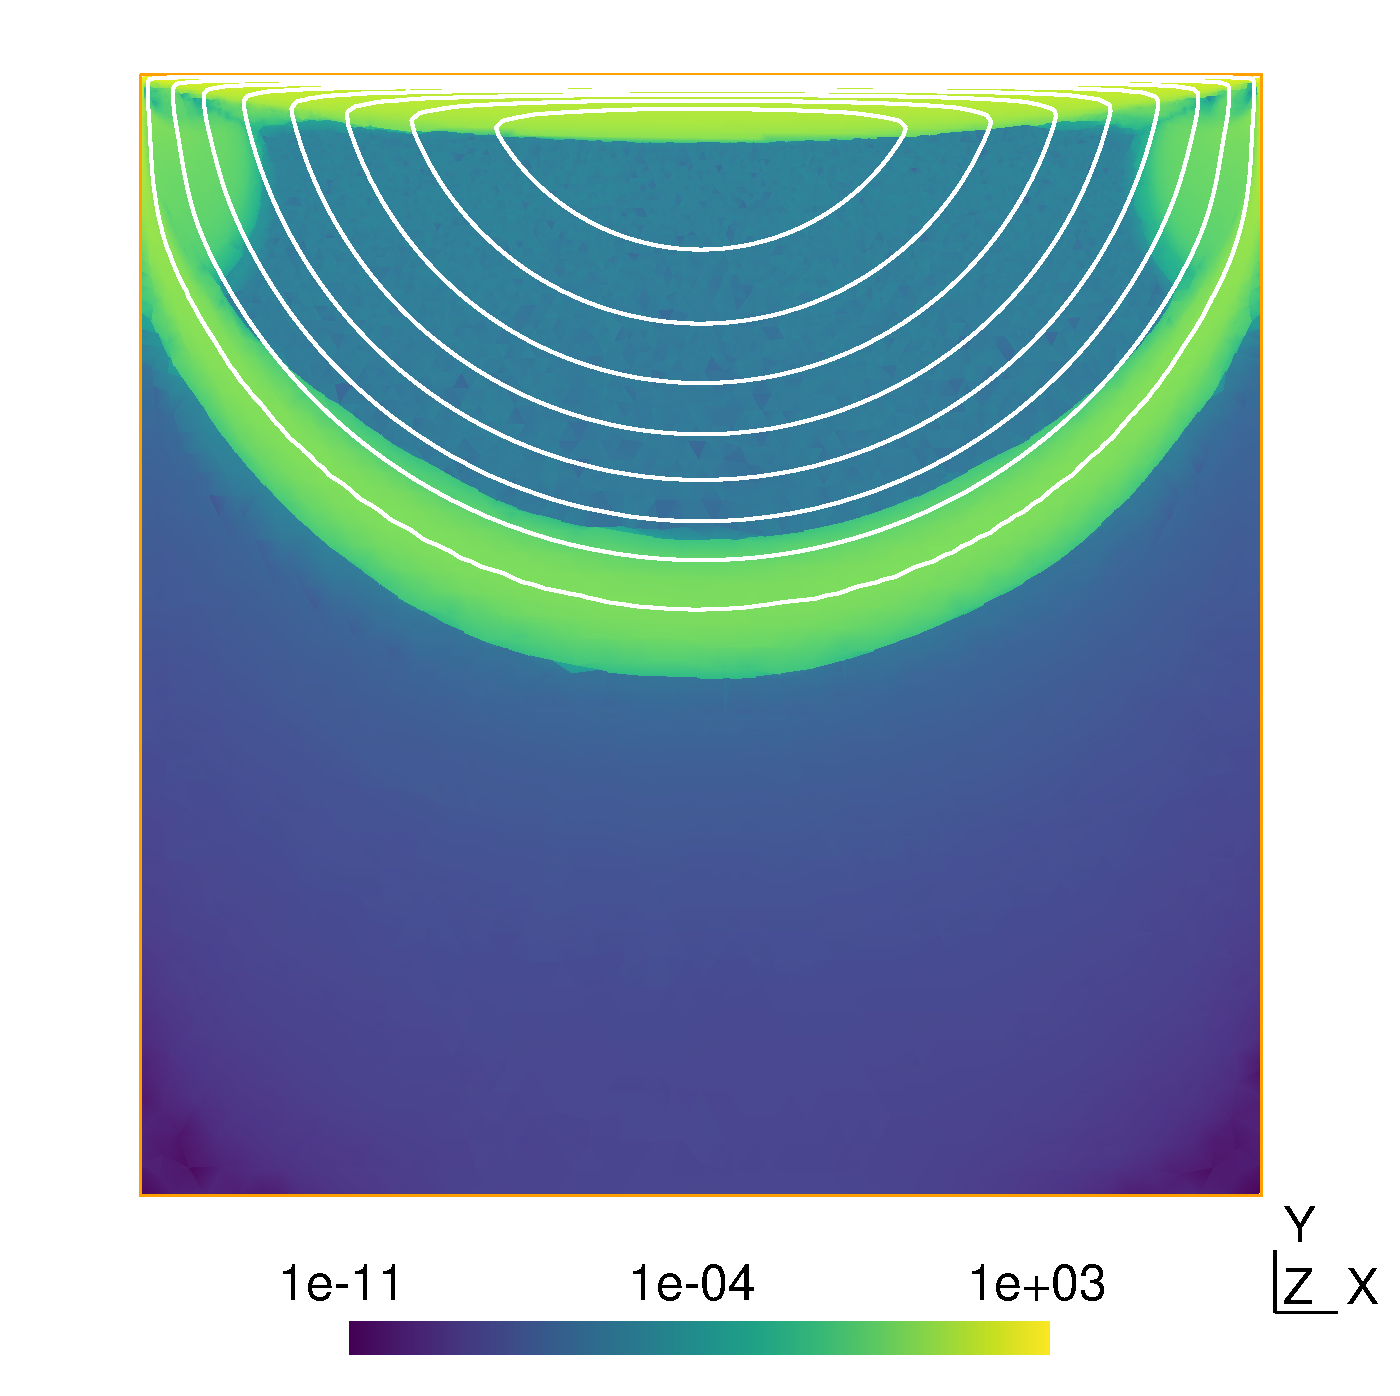
\includegraphics[width=\textwidth]{../figures/cavity_100.pdf}
        \caption{$Bn=100$}
        \label{fig:cavity100}
    \end{subfigure}
    \caption{Streamlines in white, and colormap of the strain rate norm using a logarithmic scale.}
    \label{fig:cavity}
\end{figure} 
\vfill

\pagebreak
\vfill
\begin{figure}[t]
    \centering
    \begin{subfigure}[t]{\textwidth}
        \centering
        \includesvg[width=0.9\textwidth]{../figures/profile_cavity.svg}
        \caption{Velocity profile and its derivative.}
        \label{fig:profilesCavity}
    \end{subfigure}\vspace{15pt}
    \begin{subfigure}[t]{\textwidth}
        \centering
        \includesvg[width=0.80\textwidth]{../figures/profile_papers_cavity.svg}
        \caption{Comparison with the litterature.}
        \label{fig:compareCavity}
    \end{subfigure}\vspace{15pt}
    \caption{Horizontal velocity profile along the center vertical line.}
\end{figure}
\vfill
\pagebreak

\FloatBarrier
\subsection{Modified geometry -- open cavity}

\begin{figure}[h]
    \centering
    \begin{subfigure}[t]{0.495\textwidth}
        %\includesvg[width=\textwidth]{../figures/cavity_0.svg}
        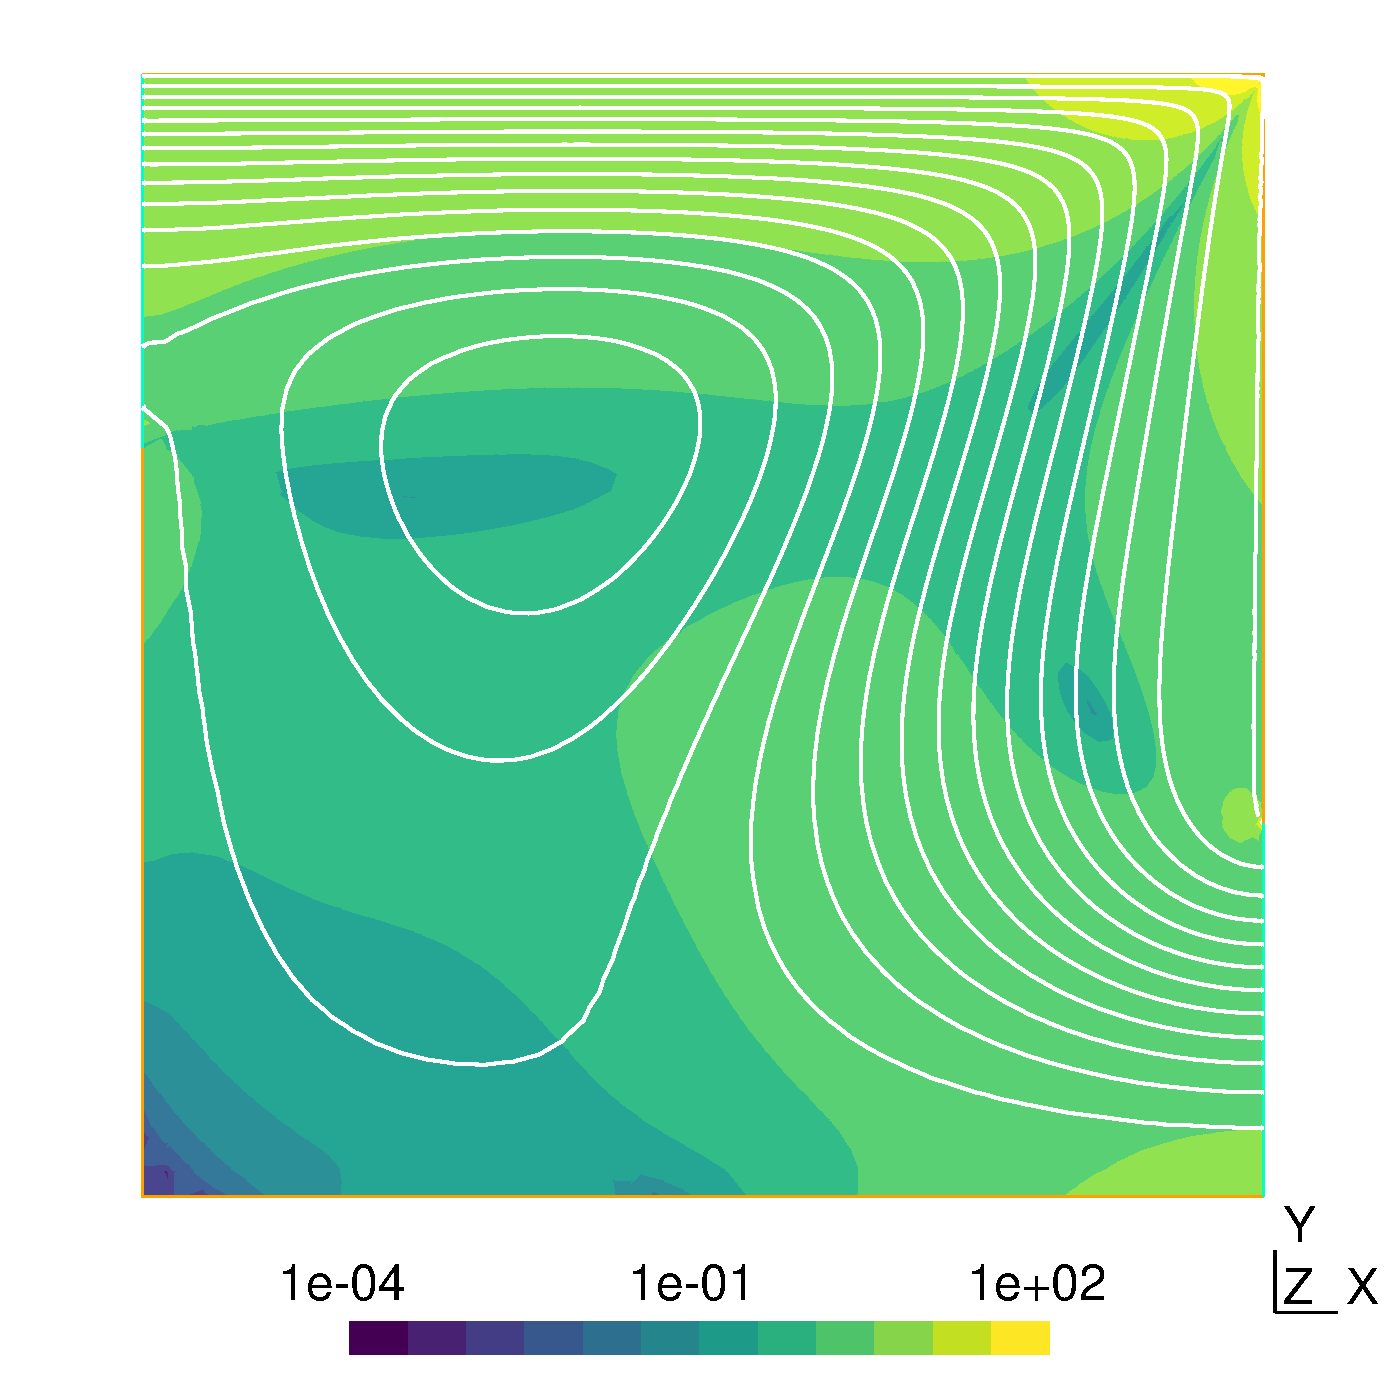
\includegraphics[width=\textwidth]{../figures/opencavity_0.pdf}
        \caption{$Bn=0$ (Newtonian fluid)}
        \label{fig:opencavity0}
    \end{subfigure}
    \begin{subfigure}[t]{0.495\textwidth}
        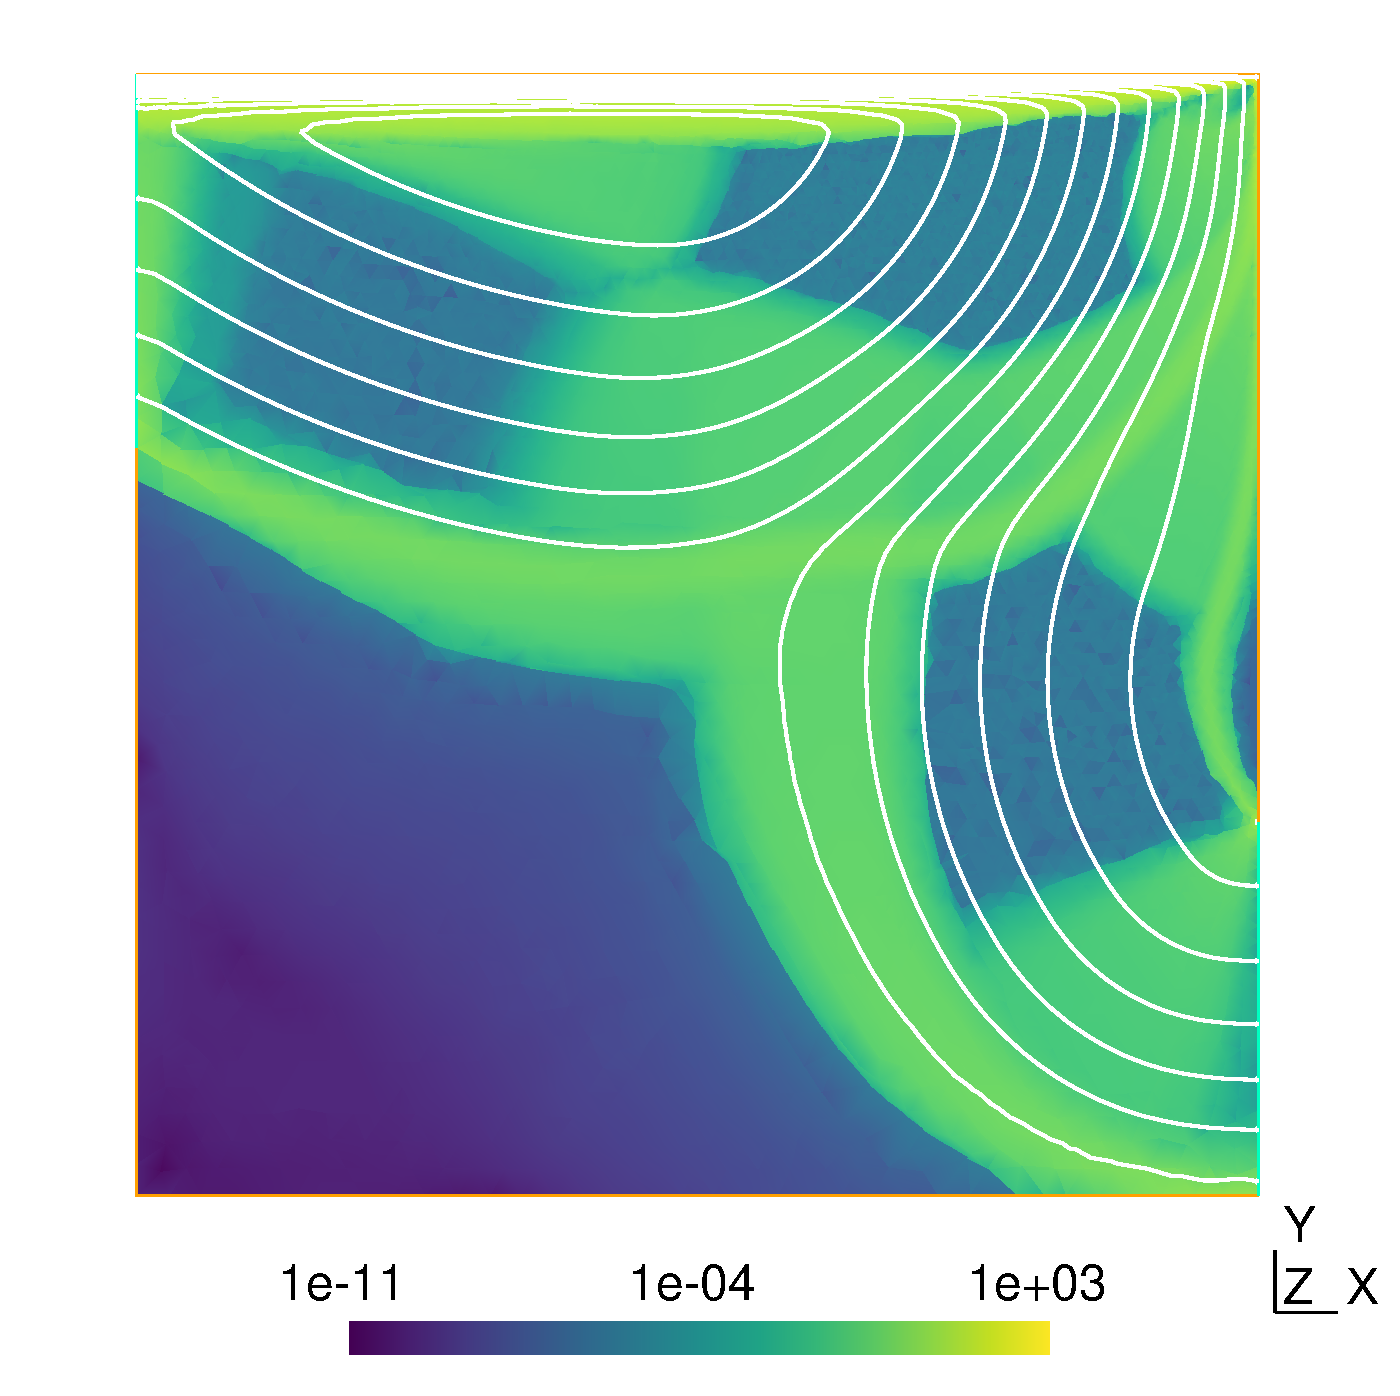
\includegraphics[width=\textwidth]{../figures/opencavity_100.pdf}
        \caption{$Bn=100$.}
        \label{fig:opencavity100}
    \end{subfigure}
    \caption{Streamlines in white, and colormap of the strain rate norm using a logarithmic scale. The mesh is made up of $14\,000$ elements, and is refined along the top and right boundaries.}
    \label{fig:opencavity}
\end{figure} 

In this exotic lid-driven cavity, there are open boundaries on the left and on the right of the cavity where no pressure difference is imposed. In the Newtonian case (\cref{fig:opencavity0}), we can also observe that the left boundary is both an inflow and an outflow, as a streamline goes around the stagnation point and goes back. 

There are 5 unyielded regions in \cref{fig:opencavity100}: a large one with no flow, 3 medium-sized ones, and a small one close to the outflow and stuck to the wall. The 4 largest seem to emerge once again from the roots of the strain rate of the Newtonian fluid flow. The pattern is broken, however, as the last, smallest region emerges from nowhere.

Finally, we observe that the two solid regions above are connected by a curve of low strain rate. It once again comes with a pressure discontinuity.

\section{Flow past an obstacle}

In our first physics lessons, we learned the usefull approximation that the drag force experienced by an object moving through a fluid is either proportional to its speed, or to the square of its speed, depending on the Reynolds number.

For a low Reynolds Newtonian fluid flow, the drag can even be exactly computed with Stokes' equations. After a few calculations, the expression of the drag force around a sphere of radius $a$ boils down to $6\pi K U_{\infty} a$ \cite{stokesSphere,stokesExpansion}: this law was already derived back in 1851 by Stokes himself. However, a dimensional analysis shows that there is always a distance $r \gtrsim a / Re$ where the convective term start to dominate \cite{lamb1945hydrodynamics,stokesExpansion}. 

For three dimensional flow, the approximation $Re\ll 1$ is of no major consequence, but in 2D, the story is quite different. There exists in fact no solution to the Stokes problem for a an unbounded flow around a disk that respects both boundary conditions far away ($\vv=U_{\infty}\mathbf{e}_1$) and around the sphere ($\vv=0$): this is the Stokes' paradox. Progress can however be made with an asymptotic expansion of the convective term of the Navier-Stokes equations \cite{stokesExpansion}.

To summarize, the flow we are considering here is bounded with slip-walls and does not attempt to reproduce an unbounded flow that is impossible to simulate because of Stokes' paradox.

\begin{figure}[ht]
    \centering
    \begin{tikzpicture}
        \tikzstyle{ground1}=[fill,pattern=north west lines,draw=none, minimum width=0.75cm,minimum height=0.2cm]
        \tikzstyle{ground2}=[fill,pattern=north east lines,draw=none, minimum width=0.75cm,minimum height=0.2cm]

        \node (wall_up) [ground1, minimum width=10cm, yshift=2cm, anchor=south] {};
        % \node[anchor=east] (wall_up_left) at (-6, 2) {}
        \draw[line width=1mm, blue!80] (wall_up.south east) -- (wall_up.south west);
        %\draw[gray, thick] (-6,2) node[black,anchor=east]{$y=H$} -- (6,2) ;

        \node (wall_down) [ground2, minimum width=10cm, yshift=-2cm, anchor=north] {};
        % \node[anchor=east] (wall_down_left) at (-6, -2) {}
        \draw[line width=1mm, blue!80] (wall_down.north east) -- (wall_down.north west);
        %\draw[gray, thick] (-6,-2) node[black,anchor=east]{$y=-H$} -- (6,-2) ;

        % \filldraw [color=black, fill=gray!30!white] (0., 0.) circle (1);
        \filldraw [color=black, fill=gray!30!white] (-0.5, -1.) rectangle (0.5,1);

        \draw[<->] (-3.0,-1.75) -- (-3.0,1.75) node [midway, right] {$H=5 h$};
        \draw[<->] (0.65,-0.95) -- (0.65,0.95) node [midway, right] {$h$};
        \draw[<->] (-0.45,1.15) -- (0.45,1.15) node [midway, above] {$h/2$};
        \draw[<->] (-4.75,-1.8) -- (4.75,-1.8) node [midway, above] {$L=10h$};

        \draw[dashed, line width=1mm, Green!100] (wall_down.north east) -- (wall_up.south east);
        \draw[dashed, line width=1mm, Red!60] (wall_down.north west) -- (wall_up.south west);

        \draw[ultra thick, ->, Red!60] (-5.5,+1.) -- (-4.5, +1.);
        \draw[ultra thick, ->, Red!60] (-5.5,+0.) -- (-4.5, +0.);
        \draw[ultra thick, ->, Red!60] (-5.5,-1.) -- (-4.5, -1.);
        \draw[ultra thick, ->, Green!100] (+4.5,+1.) -- (+5.5, +1.);
        \draw[ultra thick, ->, Green!100] (+4.5,+0.) -- (+5.5, +0.);
        \draw[ultra thick, ->, Green!100] (+4.5,-1.) -- (+5.5, -1.);

        \node (label) at (-6.5, 0.) [minimum width=3cm, color=red!60]{
            $
            \begin{aligned}
                \vv \cdot \nn &= -1\\
                \vv \cdot \tgt &= 0
            \end{aligned}
            $
        };

        \node (label) at (2.85, 1.15) [minimum width=3cm, color=blue!80]{
            $
            \begin{aligned}
                \vv\cdot \nn &= \mathbf{0}\\
                \mathbf{g} &= 0 \tgt
            \end{aligned}
            $
        };

        \node (label) at (6.5, 0.) [minimum width=3cm, color=Green!100]{
            $
            \begin{aligned}
                \mathbf{g} &= 0\nn\\
                \vv \cdot \tgt &= 0
            \end{aligned}
            $
        };

    \end{tikzpicture}
    \vspace{6pt}
    \caption{Flow around a cylinder. The inflow velocity is uniform. The outflow pressure is uniform and set to $0$. The lateral boundaries are slip-walls.}
    \label{fig:cylinderSetup}
\end{figure}

Furthermore, the disk was replaced by a square because it generates bigger "Bingham features", and therefore easier to visualize, cf. \cref{fig:cylinderSetup}. These features are specific rigid zones around the obstacle, observed by \cite{adaptiveCylinder,simulationCylinder}, and simulated here in \cref{fig:cylinder}:
\begin{itemize}
    \item A dead zone upstream and downstream, where the velocity profile is uniform.
    \item A deformation zone around the rectangle, allowing the particles to change direction and bypass the obstacle.
    \item Two \textit{pikes}, or \textit{caps}, stuck to the obstacle, pointing in the direction of the flow.
    \item Two rigid zones, called \textit{almonds} where the fluid is in solid rotation. They are lying inside the deformation zone.
\end{itemize}

In order to capture the pikes and almonds, the mesh was refined near the rectangle, and the vertical center line. The mesh size grows from $l \sim h/40$ around the obstacle, to $l \sim h/3$ in the far field (outside of \cref{fig:cylinder}). The observation is comparable to previous situations:
\begin{itemize}
    \item The unyielded zones grow in size as the Bingham number increases.
    \item Some unyielded zones are connected through valleys of low deformation, that come with a pressure discontinuity.
\end{itemize}

The interface tracking is illustrated in \cref{fig:cylinderTracking} for $Bn=\frac{\tau_0 h}{K U_{\infty}}=10$. We can see that the algorithm struggles to capture the kinks of the interfaces when the mesh is not fine enough. 

\begin{figure}
    \centering
    \begin{subfigure}[t]{0.495\textwidth}
        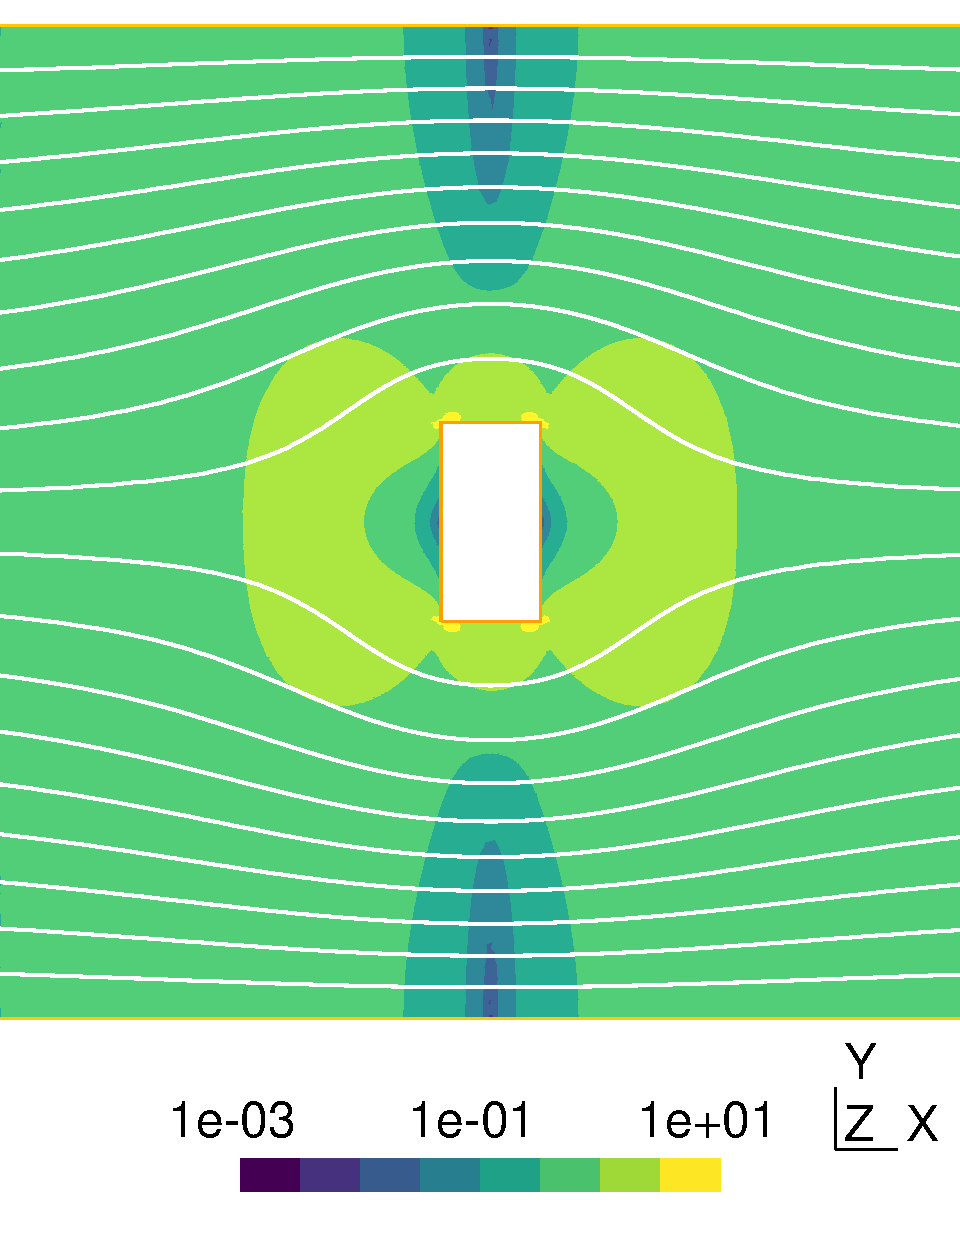
\includegraphics[width=\textwidth]{../figures/cylinder_0.pdf}
        %\caption{$Bn=0$}
        \label{fig:cylinder0}
    \end{subfigure}
    \begin{subfigure}[t]{0.495\textwidth}
        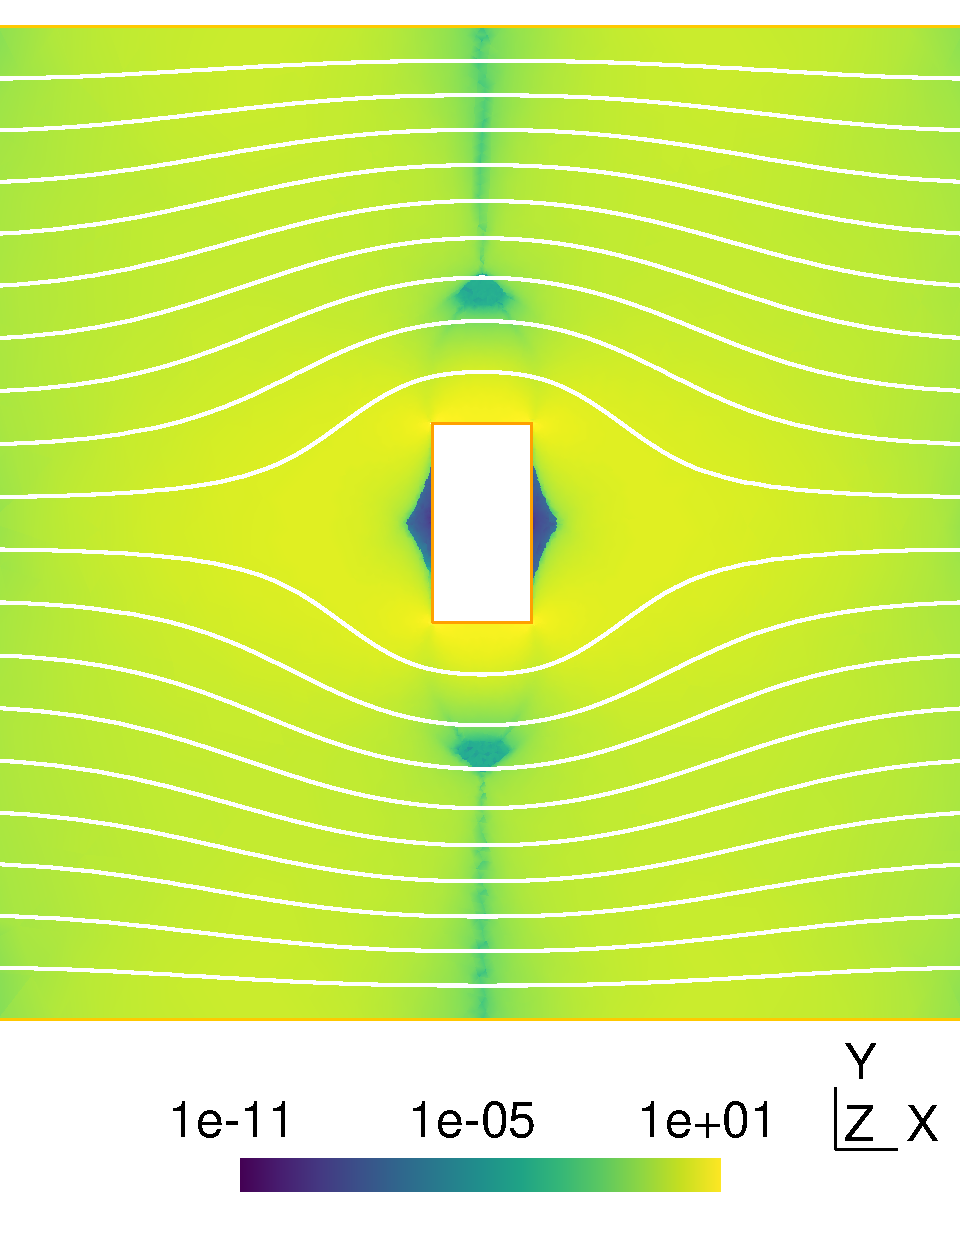
\includegraphics[width=\textwidth]{../figures/cylinder_1.pdf}
        %\caption{$Bn=1$}
        \label{fig:cylinder1}
    \end{subfigure}
    \begin{subfigure}[t]{0.495\textwidth}
        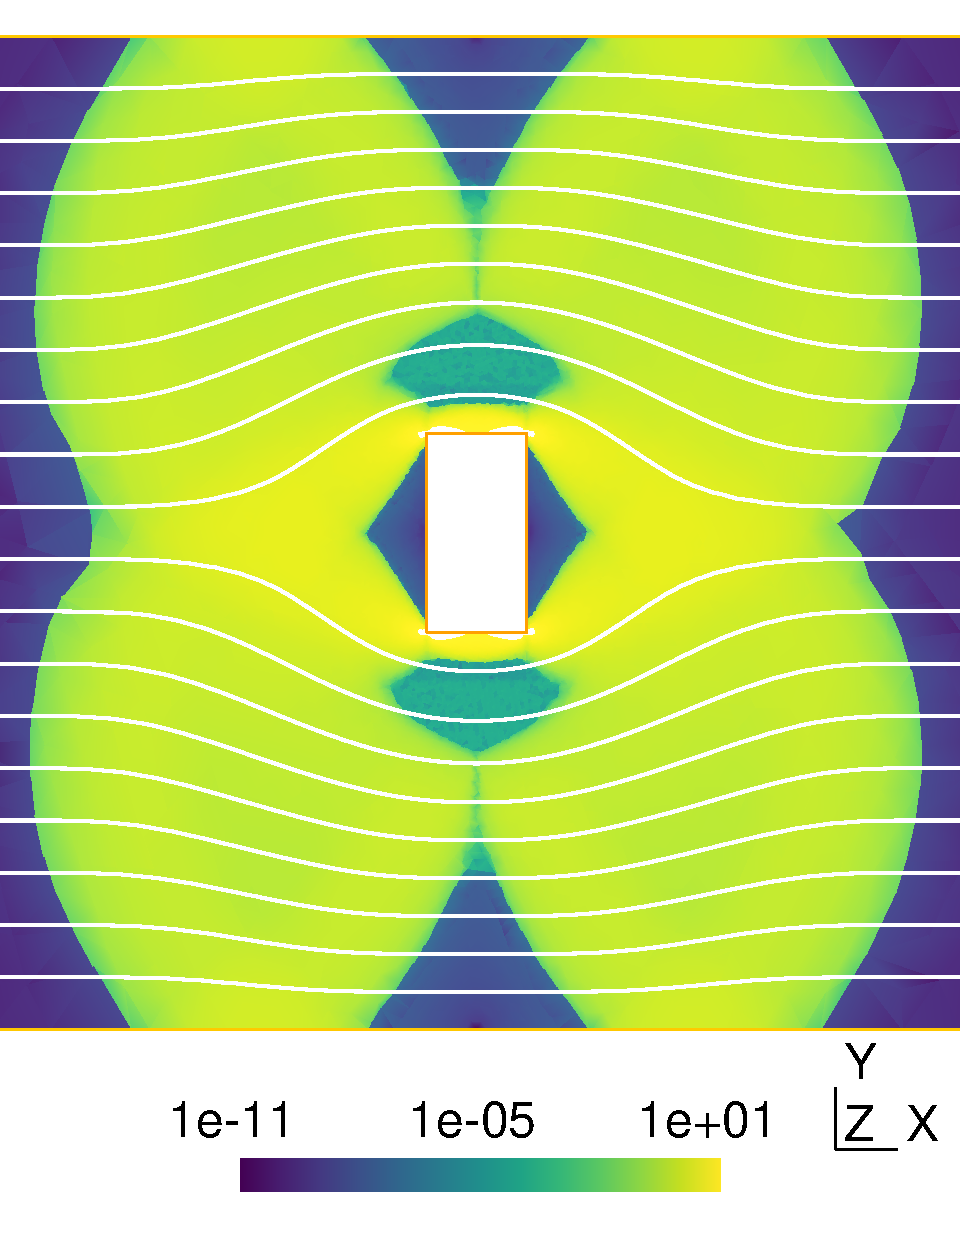
\includegraphics[width=\textwidth]{../figures/cylinder_10.pdf}
        %\caption{$Bn=10$}
        \label{fig:cylinder10}
    \end{subfigure}
    \begin{subfigure}[t]{0.495\textwidth}
        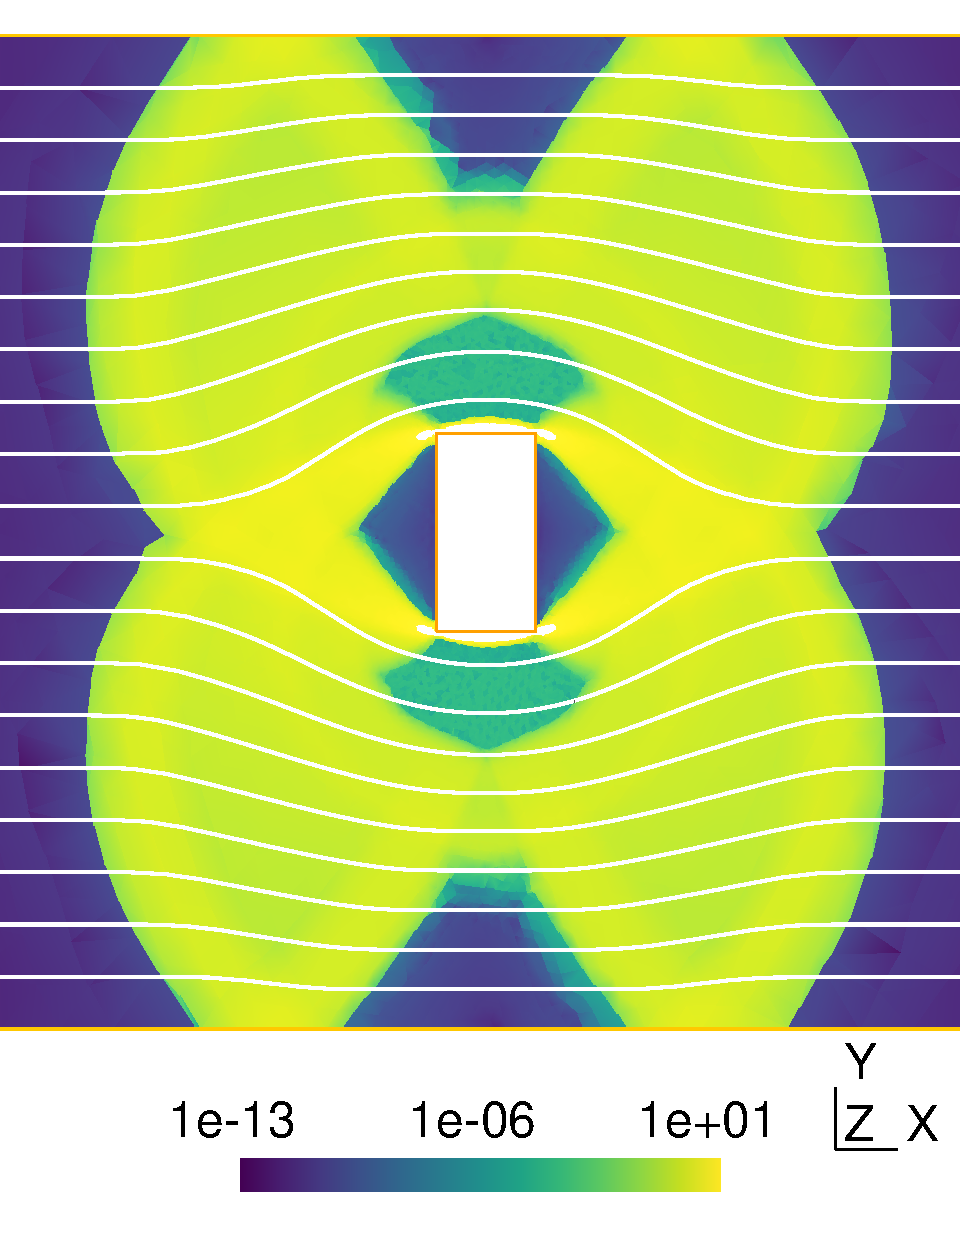
\includegraphics[width=\textwidth]{../figures/cylinder_100.pdf}
        %\caption{$Bn=100$}
        \label{fig:cylinder100}
    \end{subfigure}
    \caption{Strain rate tensor norm in log-scale, near the obstacle, for $Bn=0,1,10,100$.}
    \label{fig:cylinder}
\end{figure}

\begin{figure}
    \centering
    \begin{subfigure}[t]{\textwidth}
        \centering
        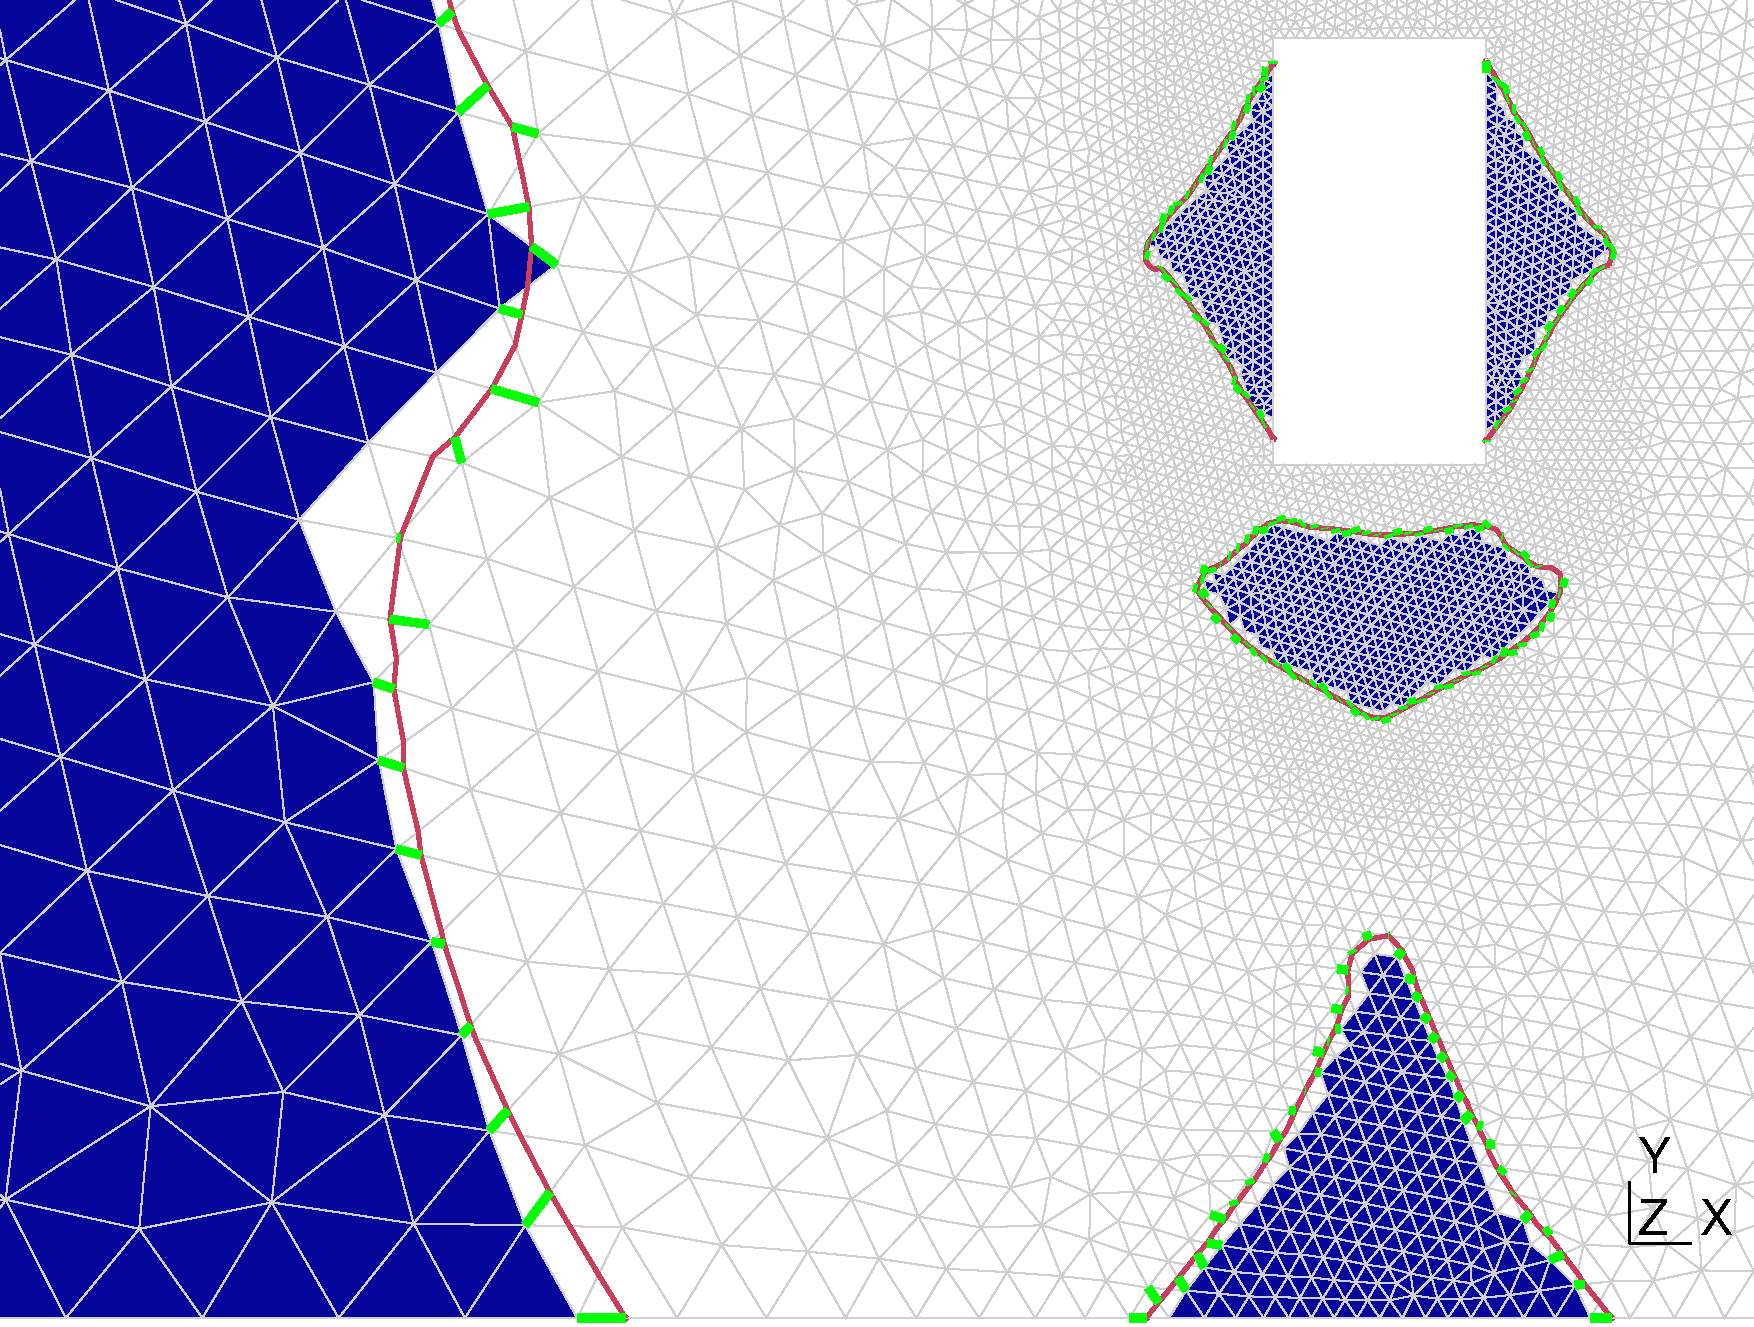
\includegraphics[width=0.85\textwidth]{../figures/cylinder_mesh.pdf}
    \end{subfigure}\vspace{6pt}
    \begin{subfigure}[t]{\textwidth}
        \centering
        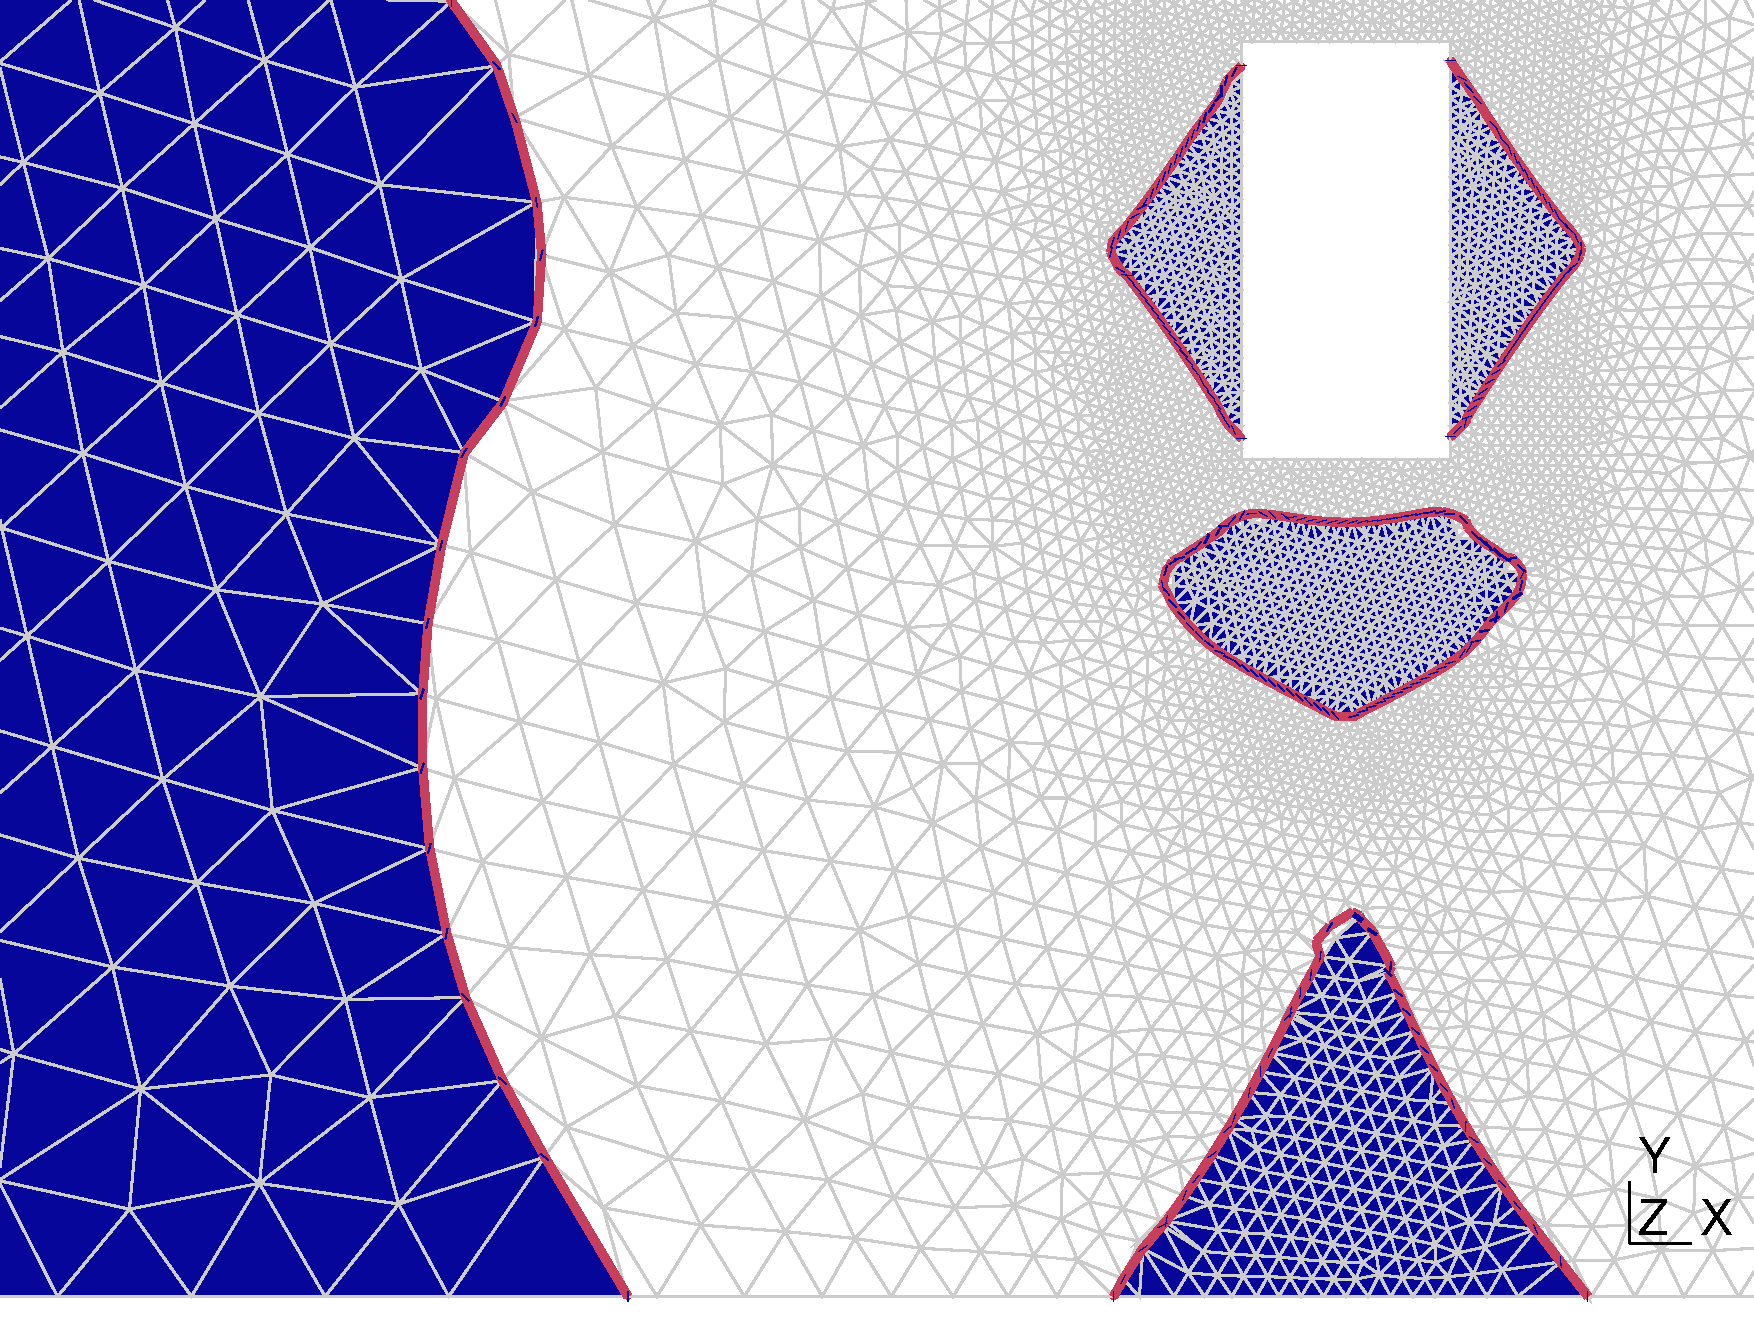
\includegraphics[width=0.85\textwidth]{../figures/cylinder_mesh_2.pdf}
    \end{subfigure}
    \caption{First and last step of the interface tracking. Predictor is colored blue, and the zero level set of the corrector is the red line. The node displacements are shown in green.}
    \label{fig:cylinderTracking}
\end{figure}

\section{Failures of the interface tracking}
\label{sec:failures}
The algorithm provides convincing results for different flows in various geometries, as shown in the previous sections. However, it is not yet sufficiently robust. A few examples will demonstrate this.

\subsection{Zero measure elements}
Some elements may end up with an area close to zero. In this case, the symmetrical velocity gradient $\gam$ becomes inconsistent, with a norm much higher than its neighbors. The \textit{caps}, triangles with two angles $\to 0$, seem to pose the most problems. Less troublesome, but still problematic, are the \textit{needles}, with one angle $\to 0$. 

An example is given in \cref{fig:failureCap}, in the simulation of a flow around a cylinder. Linear approximations in the vicinity of such triangles are unphysical, and so is the resulting interface corrector. The problem has been corrected, with relative success, by discarding the values of $\dot \gamma$ over those elements, by fixing a threshold.

In the simplest Poiseuille flow situation, a similar situation can unfortunately arise. By iterating the algorithm more than necessary, we obtain elements with negative aera. This makes the optimization problem \eqref{eq:functional2D} non-convex, and thus impossible to solve by the interior-point algorithm.

\begin{figure}
    \centering
    \begin{subfigure}[t]{0.55\textwidth}
        \centering
        \includesvg[width=0.90\textwidth]{../figures/negative_1.svg}
        \caption{Upper interface of the solid plug of a Poiseuille flow. The triangle with negative Jacobian is colored red. The numerical values indicate the average of $\dot\gamma$ over each element. The node displacements (upwards) are magnified 100 times.}
    \end{subfigure}\vspace{6pt}
    \begin{subfigure}[t]{0.55\textwidth}
        \centering
        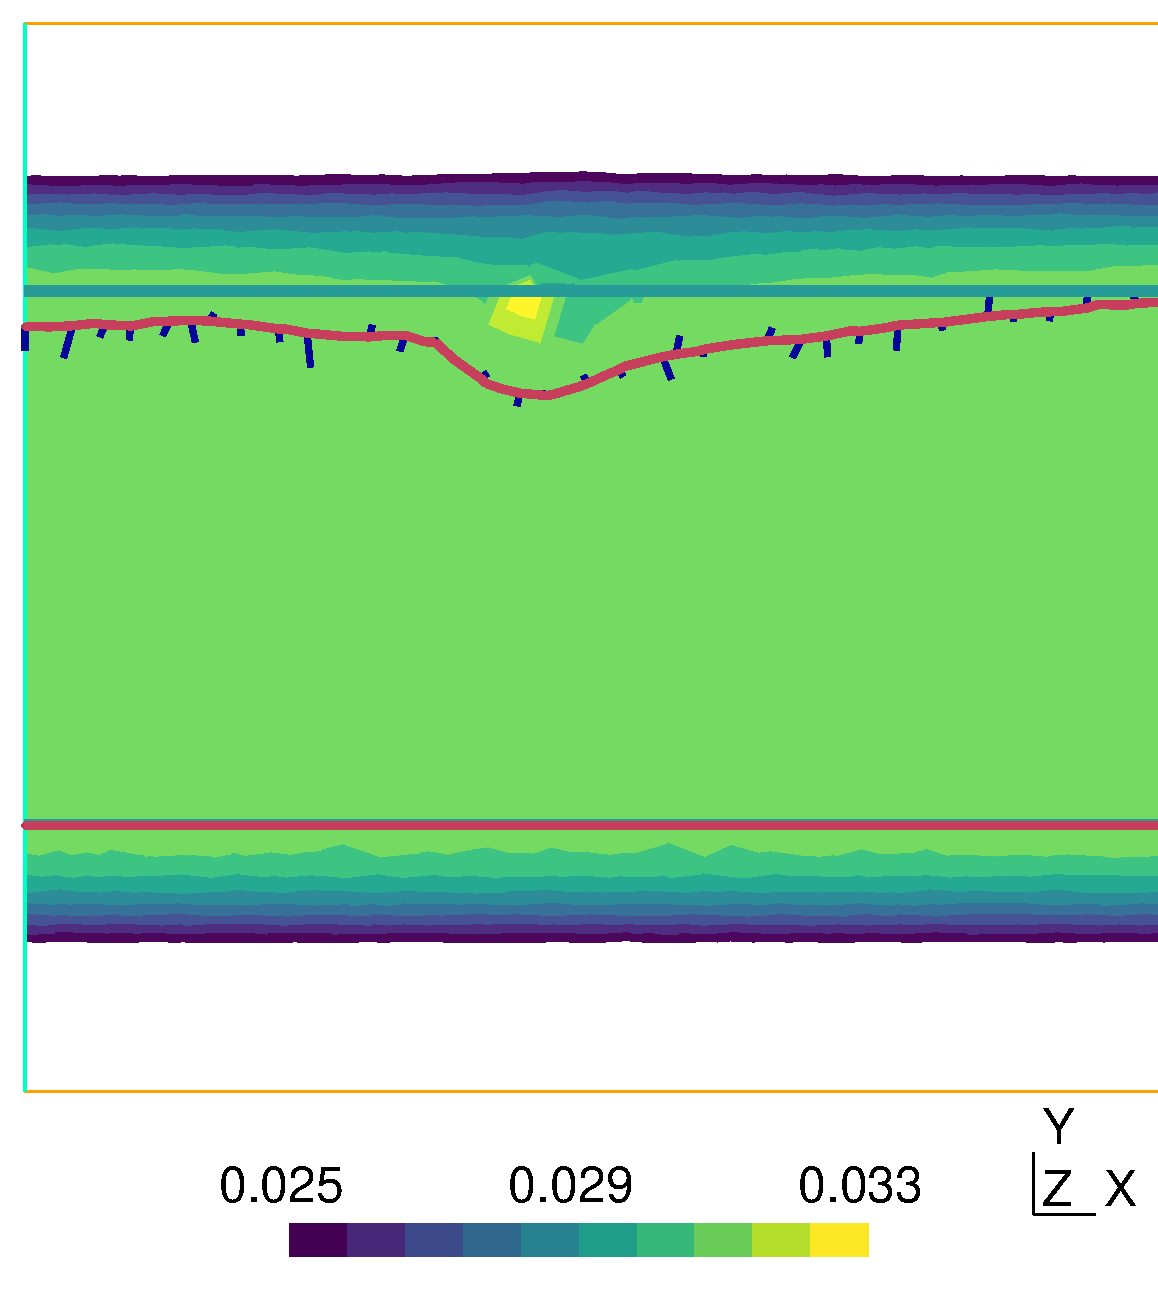
\includegraphics[width=0.90\textwidth]{../figures/negative_2.pdf}
        \caption{Colormap of the velocity field $\|\vv\|$ after the next iteration. The finite element solution is deteriorated, along with the next interface corrector.}
    \end{subfigure}\vspace{6pt}
    \caption{Impact of a negative Jacobian on the solution accuracy.}
    \label{fig:failureNegative}
\end{figure}

\begin{figure}
    \centering
    \begin{subfigure}[t]{0.495\textwidth}
        \includesvg[width=\textwidth]{../figures/issue_1.svg}
        \caption{Colormap of the strain rate tensor norm.}
    \end{subfigure}
    \begin{subfigure}[t]{0.495\textwidth}
        \includesvg[width=\textwidth]{../figures/issue_2.svg}
        \caption{Strain rate norm $T_{i,g}$ at the Gauss points.}
    \end{subfigure}\vspace{6pt}
    \begin{subfigure}[t]{0.495\textwidth}
        \includesvg[width=\textwidth]{../figures/issue_3.svg}
        \caption{Outliers in a very small elements.}
    \end{subfigure}
    \begin{subfigure}[t]{0.495\textwidth}
        \includesvg[width=\textwidth]{../figures/issue_4.svg}
        \caption{Inconsistent linear approximation.}
    \end{subfigure}\vspace{6pt}
    \caption{Bad estimation of the interface due to deformation anomalies in degenerate triangles.}
    \label{fig:failureCap}
\end{figure}

\subsection{Deformations $\dot\gamma$ of totally different scales}
%This second issue concerns the very idea of the method rather than its implementation. 
Based on a $C^2$ discontinuity, the algorithm searches for the tangent plane to $\dot \gamma$ from the yielded side. However, the slope of this plane can cover several orders of magnitude at different locations of the interface, and in a non continuous way.

Let's start with flow in a curved channel. The deformation varies significantly radially, and much less in the tengential direction. Near corners, the linear approximation has no chance of being accurate. This is detailled in \cref{fig:failureCorner}. The average of those different linear approximation generates a bulge instead the desired sharp corner.

A second illustration is provided with the lid-driven cavity flow. For the occasion, a new simulation was carried out, with a mesh size $250$ times smaller than the height of the cavity near the corners. \Cref{fig:failureRoot} shows that $\dot \gamma$ does not vary at all with the same intensity at different positions around the solid region. Along the black circles, the strong variations allow us to easily determine the interface: $5$ to $6$ orders of magnitude spanned over a short distance. However, along the white lines, the situation is less clear-cut as the change is smoother: only three $3$ orders of magnitude over a comparable distance. More importantly, linear approximations in this zone generate a virtual field $\varphi$ positive everywhere on its support. This issue could perphaps be resolved by extending the support.

\begin{figure}
    \centering
    \begin{subfigure}[t]{0.495\textwidth}
        %\includesvg[width=\textwidth]{../figures/corner_5.svg}
        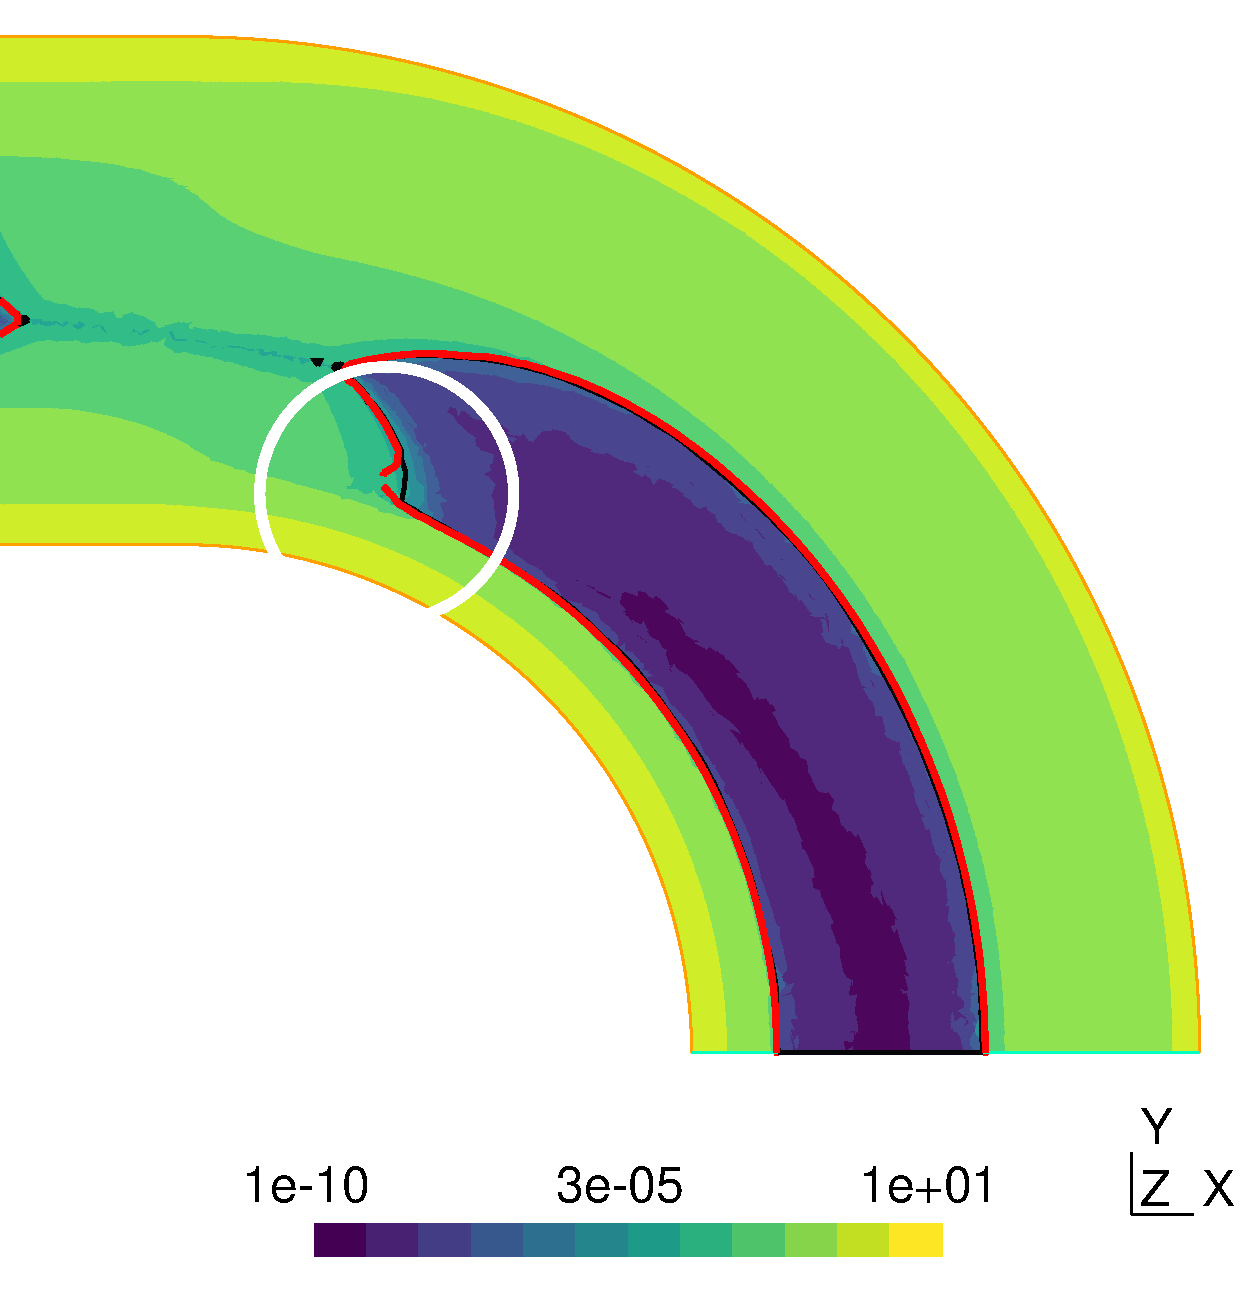
\includegraphics[width=\textwidth]{../figures/corner_5.pdf}
        \caption{Colormap of the strain rate tensor norm. The relevant corner is circle in white.}
    \end{subfigure}
    \begin{subfigure}[t]{0.495\textwidth}
        \includesvg[width=\textwidth]{../figures/corner_4.svg}
        \caption{Colormap of the virtual field, whose zero level set (red) is the interface corrector.}
    \end{subfigure}\vspace{6pt}
    \begin{subfigure}[t]{0.325\textwidth}
        \includesvg[width=\textwidth]{../figures/corner_1.svg}
    \end{subfigure}
    \begin{subfigure}[t]{0.325\textwidth}
        \includesvg[width=\textwidth]{../figures/corner_2.svg}
    \end{subfigure}
    \begin{subfigure}[t]{0.325\textwidth}
        \includesvg[width=\textwidth]{../figures/corner_3.svg}
    \end{subfigure}\vspace{6pt}
    \caption{Misestimation of the interface near sharp corners. The interface predictor and corrector are the black and red curves. The lower figures show the linear approximation on three neighbouring patches. Note the difference in scale for each patch.}
    \label{fig:failureCorner}
\end{figure}


\begin{figure}
    \centering
    \begin{subfigure}[t]{0.495\textwidth}
        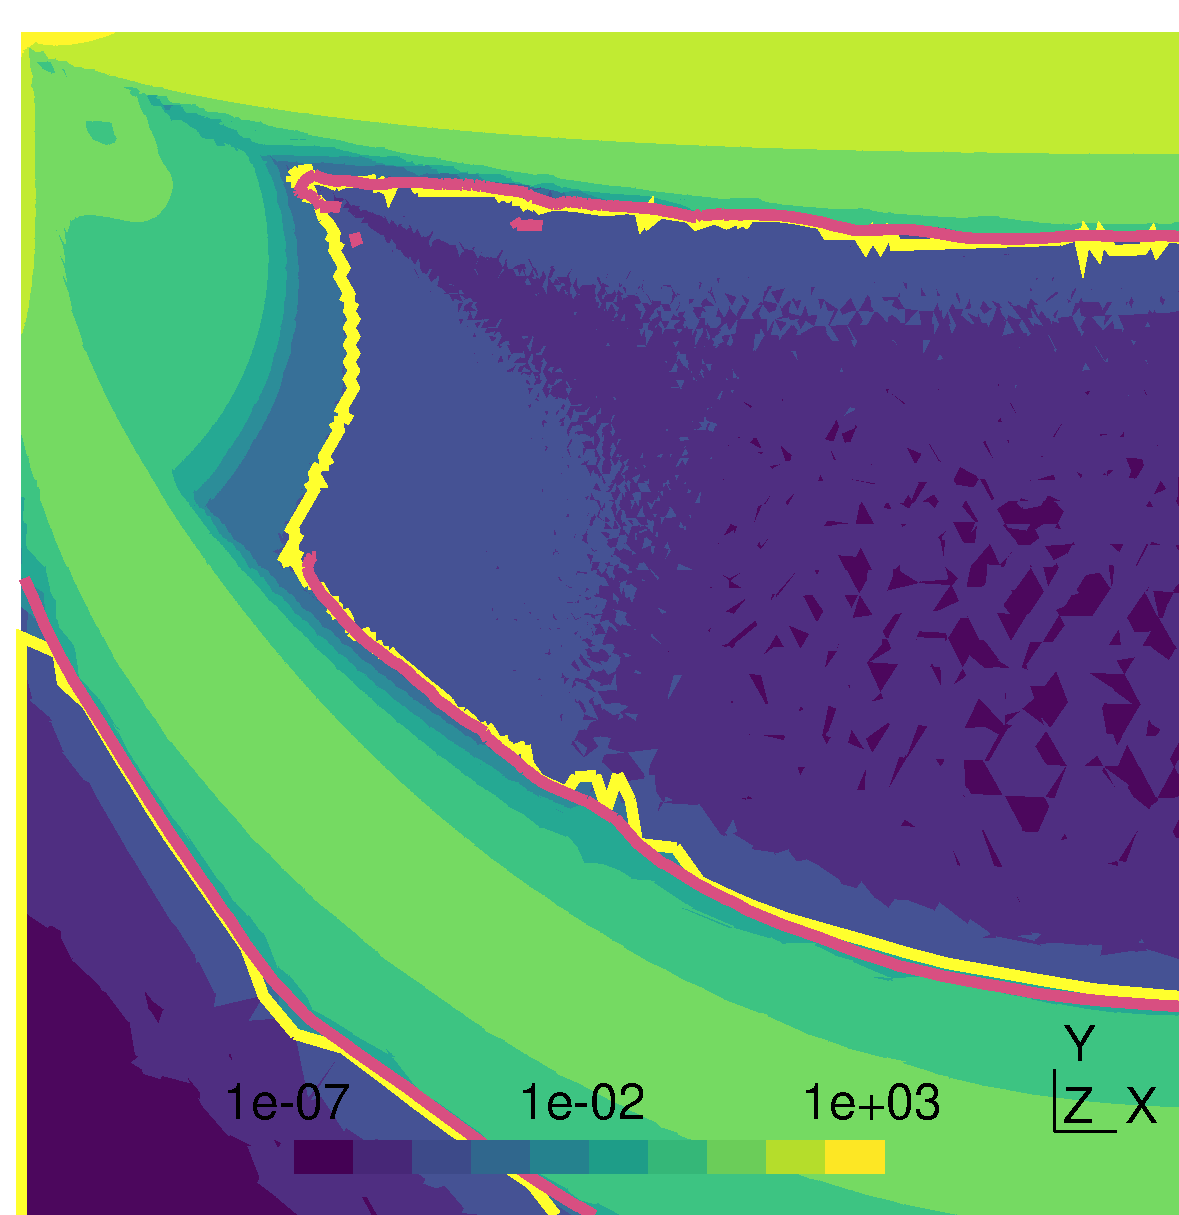
\includegraphics[width=\textwidth]{../figures/correction_1.pdf}
        \caption{Predictor in yellow, corrector in red.}
    \end{subfigure}
    \begin{subfigure}[t]{0.495\textwidth}
        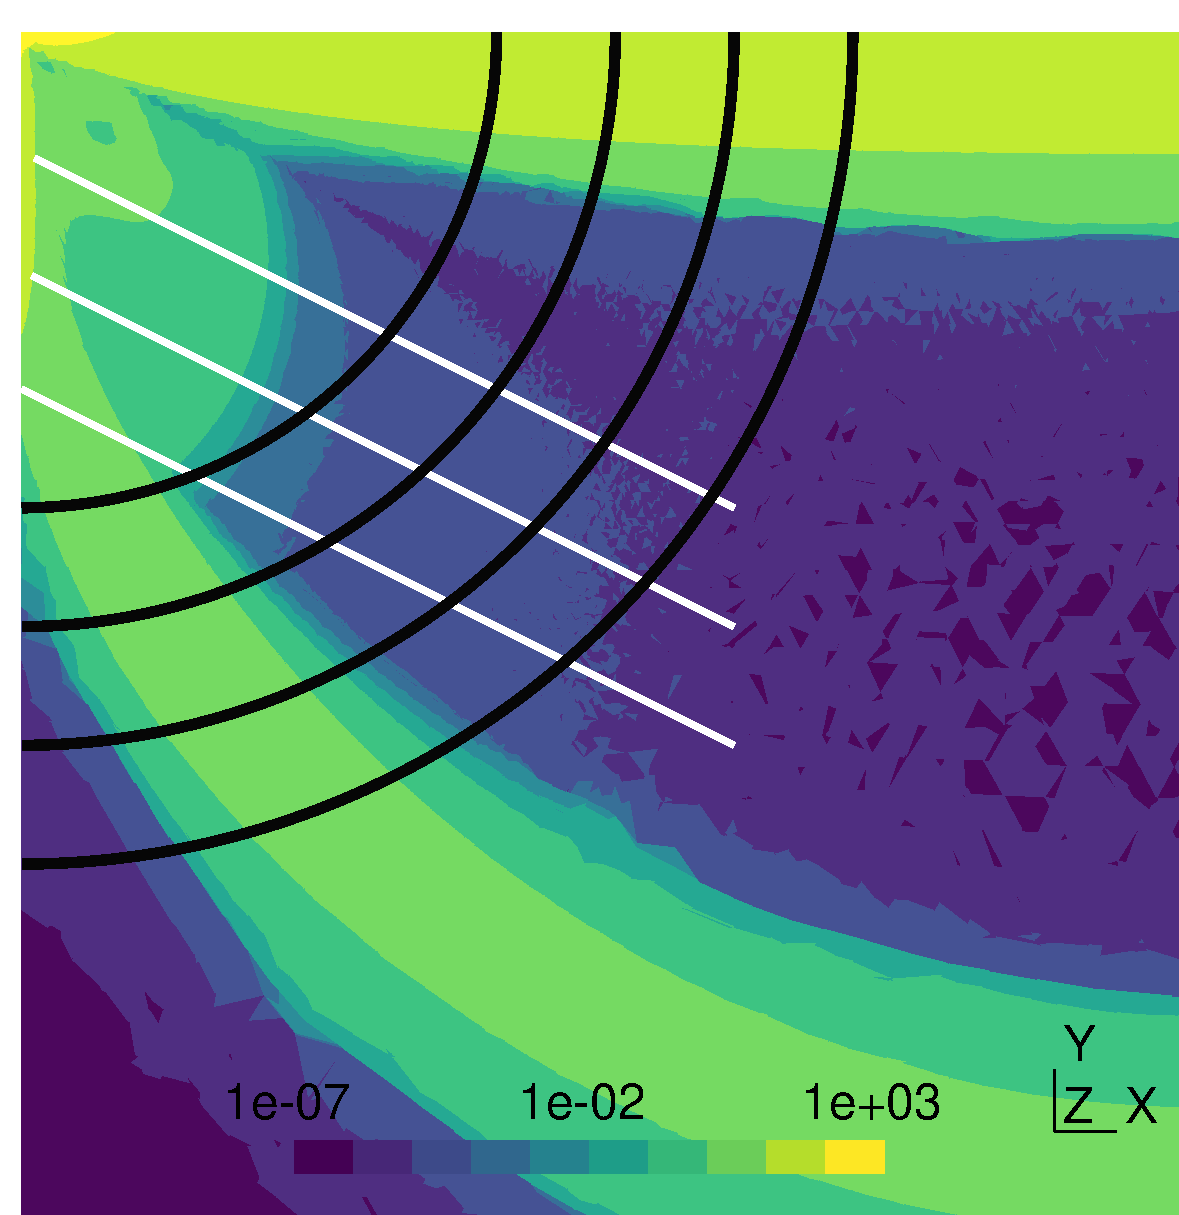
\includegraphics[width=\textwidth]{../figures/correction_2.pdf}
        \caption{Parametric curves: lines and circles.}
    \end{subfigure}
    \begin{subfigure}[t]{\textwidth}
        \includesvg[width=\textwidth]{../figures/correction_3.svg}
    \end{subfigure}
    \begin{subfigure}[t]{\textwidth}
        \includesvg[width=\textwidth]{../figures/correction_4.svg}
    \end{subfigure}
    \caption{Interrogations about the smoothness of the strain rate norm $\|\mathbf{D}\|=\dot \gamma/2$. Parametric curves are shown above in the domain $\Omega$, and the evaluation of $\|\mathbf{D}\|$ along them is shown below.}
    \label{fig:failureRoot}
\end{figure}

\FloatBarrier
\addcontentsline{toc}{chapter}{Conclusion}
\chapter*{Conclusion}

In this study, we modeled the flow of yield stress fluid, which, as a reminder, behaves as a solid under low stress, and as a liquid otherwise. More specifically, we considered the Bingham constitutive model to close our system of PDE's. The resulting non-linearity was handled by expressing the problem as an energy minimization, that was later solved with an interior-point algorithm.

This study focused on the correct management of the physical interface, that arise due to Bingham's constitutive law. The aim was therefore to obtain a topologically correct mesh, by placing nodes precisely on the interface. 

On one hand, the 1D case allowed us to familiarize ourselves with the equations and the optimization solver, but also to develop a technique that recovers the interface. The core of this thesis, on the other hand, is the simulation of various 2D flows with the astonishing features, typical of yield stress fluids, like the rigid rotating regions. %and the filaments of pressure discontinuities.

However, the algorithm is not yet mature. It is not yet capable of iterating and stopping autonomously while maintaining a conformal mesh. Each simulation was therefore stopped manually based on a visual check. The cases of failure examined in detail in \cref{sec:failures} give a good idea of the avenues to follow to make it more robust. 

The treatment of interface corners is probably the first task at hand, as they appear in almost every case. A better understanding of filaments with pressure discontinuities, which regularly appear at the corners, is the first step towards improvement. It is fair to assume that those corners are generally kinks (instantaneous change of direction), and maybe cusps (instantaneous u-turn) when filaments emerge from the rigid zone.

An equally important work is to seriously investigate the regularity of the solution. Ideally, we would like to obtain a proof of the discontinuity level (always $C^1$, never $C^2$ ?) to ensure a solid mathematical foundation for the reconstruction method.

If a third improvement had to be mentionned, it would undoubtedly concern the yield tolerance parameter $\epsilon$. The algorithm would be much more efficient and accurate if it were able to detect the change in scale of the deformation field $\dot \gamma$ on its own. This could be achieved, for example, by searching for a sudden drop in $\dot \gamma$, as illustrated in \cref{fig:failureRoot}.

Mesh deformation really improves the quality of the solution and avoids the pitfall of mesh refinement But this should be quantified with a convergence analysis, for example, to get a clearer picture of the situation. The idea of extreme mesh deformation could be push even further, by pushing the nodes away from solid to the liquid regions. This would densify the mesh were large gradients occur, and coarsen it were uniform and rotational motion happen. The velocity field would be well resolved there anyway, since it is either constant or linear.

%\nocite{*}
%\printbibliography
% \printbibliography[type=book,heading=subbibliography,title={Book Sources}]
% \printbibliography[nottype=book, nottype=online, heading=subbibliography,title={Article Sources}]
% \printbibliography[type=online,heading=subbibliography,title={Online Sources}]


\bibliographystyle{siamplain}
\bibliography{main.bib}


%%%%%%%%%%%%%%%%%%%%%%% - Curvilinear coordinates START - %%%%%%%%%%%%%%%%%%%%%%%
% \appendix
% \chapter{Curvilinear coordinates}
% \label{appendix:curvilinear}

% In axisymmetric cylindrical coordinates, the solution only depends on the radial and axial coordinates $r, z$. We also assume that the velocity field has no tangential component.

% \begin{align}
%     \begin{bmatrix}
%         x(r, \theta=0, z) \\
%         y(r, \theta=0, z) \\
%         z(r, \theta=0, z) \\
%     \end{bmatrix} &=
%     \begin{bmatrix}
%         r \\
%         0 \\
%         z
%     \end{bmatrix}\\
%     \uu(r, z) &= u_r(r, z) \mathbf{e}_r + u_z(r, z) \mathbf{e}_z\\
%     \left(\nabla \: \phi\right)_{\text{Cyl}} &= \nabla_{\boldsymbol\xi} \phi \; \cdot \dv{\boldsymbol \xi}{\mathbf{x}} \cdot \dv{\mathbf{x}}{(r, z)}\\
%     \nabla \cdot \vv &= \pdv{u_r}{r} + \frac{u_r}{r} + \pdv{u_z}{z}\\
%     \|\gam(u, v)\|_{\text{Cyl}}^2 &= 2 \bigg(\pdv{u_r}{r}\bigg)^2 + 2\bigg(\frac{u_r}{r}\bigg)^2 + 2\bigg(\pdv{u_z}{r}\bigg)^2 + \bigg(\pdv{u_r}{z} + \pdv{u_z}{r}\bigg)^2
% \end{align}

% Polar coordinates provide quite similar equations. Here again, we assume axisymmetry and the absence of azimuthal velocity.
% \begin{align}
%     \begin{bmatrix}
%         x(r, \theta, \varphi=0) \\
%         y(r, \theta, \varphi=0) \\
%         z(r, \theta, \varphi=0)
%     \end{bmatrix} &=
%     \begin{bmatrix}
%         r \sin{\theta} \\
%         0\\
%         r \cos{\theta} \\
%     \end{bmatrix}\\
%     \uu(r, z) &= u_r(r, \theta) \mathbf{e}_r + u_\theta(r, \theta) \mathbf{e}_\theta\\
%     \left(\nabla \: \phi\right)_{\text{Pol}} &= \nabla_{\boldsymbol\xi} \phi \; \cdot \dv{\boldsymbol \xi}{\mathbf{x}} \cdot \dv{\mathbf{x}}{(r, \theta)} \\
%     \nabla \cdot \vv &= \frac{1}{r^2}\pdv{(r^2 u_r)}{r} + \frac{1}{r\sin\theta} \pdv{(u_\theta \sin \theta)}{\theta}\\
%     \|\gam(u, v)\|_{\text{Cyl}}^2 &= 2 \bigg(\pdv{u_r}{r}\bigg)^2 + 2\bigg(\frac{1}{r}\pdv{u_\theta}{\theta} + \frac{u_r}{r}\bigg)^2 + 2\bigg(\frac{u_r}{r} + \cot \theta \frac{u_\theta}{r}\bigg)^2 \nonumber\\
%     &+ \bigg(\frac{1}{r}\pdv{u_r}{\theta} \pdv{u_\theta}{r} - \frac{u_\theta}{r}\bigg)^2
% \end{align}
%%%%%%%%%%%%%%%%%%%%%%%% - Curvilinear coordinates END - %%%%%%%%%%%%%%%%%%%%%%%%

%
\includepdf[pages=-]{back_page.pdf}

\end{document}


    \draw[gray, thick] (2,0) -- (6,0);
    \draw[gray, thick, dotted] (-2, 0) -- (2, 0);
    \filldraw[black] (0,-1) circle (1pt);
    \draw[black] (0,-1) circle ({sqrt(5)});
    \draw[<->] (0, -0.1) -- (0, -0.9) node[midway, right] {$\Bar{z} + z^*$};
    \draw[<->] ({-sqrt(5)+0.1}, -1) -- (-0.1, -1) node[midway, below] {$R$};


    \begin{split}
        I_2(\mathbf{A}) &\coloneqq \frac{1}{2} \left[\Tr(\mathbf{A}^2) - \big(\Tr(\mathbf{A})\big)^2\right]
    \end{split}
    \quad \implies
    \begin{split}
        \dot \gamma &\coloneqq \sqrt{I_2(\gam)} = \sqrt{\frac{1}{2} \, \gam : \gam} = \sqrt{2 \mathbf{D} : \mathbf{D}}\\
        \tau &\coloneqq \sqrt{I_2(\boldsymbol\tau)} = \sqrt{\frac{1}{2} \, \boldsymbol\tau : \boldsymbol\tau}
    \end{split}
